% IEEE T-ASE regular-paper format: 10 pt, US Letter, two columns.
\documentclass[10pt,journal,letterpaper]{IEEEtran}

% Complete manuscript: sections and references are embedded in this file.
% The default build includes all authors and both corresponding authors.
% For anonymous review, define \TASEanonymousreview before compiling this file.
\newif\ifTASEanonymous
\ifdefined\TASEanonymousreview
  \TASEanonymoustrue
\else
  \TASEanonymousfalse
\fi
\newif\ifTASEshowrevisions
\TASEshowrevisionsfalse

\hyphenation{op-tical net-works semi-conduc-tor}
\usepackage{graphicx}
\graphicspath{{figures/}}
\usepackage{algorithm}
\usepackage{algorithmic}
\usepackage{amsmath}
\usepackage{booktabs}
\usepackage{cite}
\usepackage{bm}
\usepackage{amsfonts}
\usepackage{xcolor}
% Keep IEEEtran's figure/table captions; caption=false is essential here.
\usepackage[caption=false,font=footnotesize]{subfig}
\usepackage{float}
\usepackage{multirow}
\usepackage[hidelinks]{hyperref}
\usepackage{orcidlink}
\newcommand{\rev}[1]{\ifTASEshowrevisions\textcolor{blue}{#1}\else#1\fi}
\newcommand{\newrev}[1]{#1}
\renewcommand{\thesubfigure}{\alph{subfigure}}
% Reuse IEEEtran's abstract typography for the required practitioner note.
\newenvironment{IEEEpractitioners}
  {\renewcommand{\abstractname}{Note to Practitioners}\begin{abstract}}
  {\end{abstract}}
\hypersetup{
  pdftitle={Multi-Balancing-Agent Reinforcement Learning for Charging Control of Lithium-ion Batteries},
  pdfauthor={},
  pdfsubject={IEEE Transactions on Automation Science and Engineering manuscript},
  pdfkeywords={Charging control, lithium-ion batteries, multi-agent reinforcement learning, state-of-charge balancing}
}

\begin{document}

\title{Multi-Balancing-Agent Reinforcement Learning for Charging Control of Lithium-ion Batteries}


\maketitle
\begin{abstract}
Lithium-ion batteries are widely used in electric vehicles and energy storage systems because of their high energy density, long cycle life, 
and low self-discharge rate. However, cell-to-cell differences can reduce usable capacity, charging efficiency, and safety, making fast charging with state-of-charge (SOC) balancing a challenging control problem. 
This paper proposes a multi-balancing-agent reinforcement learning (MBA-RL) framework for coordinated battery-pack charging without a dedicated equalization topology. 
MBA-RL formulates cell-level charging as a cooperative multi-agent control problem, allowing independently regulated cell currents to jointly optimize charging progress and pack-level SOC balance. 
% A model-based safety mechanism further screens requested currents against predicted voltage, temperature, and SOC limits before execution. 
Extensive experiments show that MBA-RL reduces accumulated SOC imbalance by 12.65\% and 10.82\% compared with shared independent Q-learning and centralized deep Q-learning, respectively. 
The safety mechanism satisfies the prescribed constraints in all tested cases, while incorporating it during training further improves task completion and SOC balancing.
\end{abstract}
\begin{IEEEpractitioners}
This work aims to support the practical development of intelligent charging strategies for lithium-ion battery packs with independently controllable cell currents. In real applications, cell-to-cell differences in aging and operating conditions can cause uneven charging progress, making it difficult to achieve fast charging and SOC balance simultaneously. Conventional balancing approaches typically rely on dedicated equalization circuits to redistribute or dissipate energy among cells. The proposed MBA-RL framework provides an alternative by coordinating the charging current of each cell directly through multi-agent reinforcement learning. Engineers can use the learned controller to adjust cell-level charging currents according to local voltage, temperature, and SOC information, while a model-based safety mechanism screens the requested currents before execution. The controller is trained offline and can then be deployed without online parameter updates. This framework is suitable for intelligent battery management and fast-charging systems that support independent cell-current regulation, particularly when cell inconsistency becomes significant during operation. In future work, we will further validate the proposed approach on hardware platforms and extend the framework to larger battery packs with coupled electrical, power, and thermal constraints.
\end{IEEEpractitioners}
\begin{IEEEkeywords}
Charging control, lithium-ion batteries, multi-agent reinforcement learning, SOC balancing.
\end{IEEEkeywords}

% Begin merged section: 01_introduction.tex
\section{Introduction}

Lithium-ion batteries are widely used in electric vehicles (EVs) and energy storage systems because of their high energy density, long cycle life, and low self-discharge rate \cite{1}. In practical applications, a single cell cannot meet the voltage and capacity requirements of large-scale battery systems \cite{3, 4}. Battery packs therefore consist of many individual cells connected in series and parallel. Differences in manufacturing and operating conditions lead to variations in cell states and aging characteristics, which can reduce the usable capacity and durability of the battery pack \cite{4}. Related battery-management research has addressed capacity degradation by accounting for the coupling between calendar and cycling aging \cite{liu2024degradation}, and the co-estimation of state of charge (SOC) and state of energy (SOE) using a model-data fused framework \cite{duan2026coestimation}. Hybrid physics-informed neural networks have also been developed for battery prognosis and fleet management under large load variations \cite{fricke2026prognosis}. Effective charging control must therefore achieve fast charging while maintaining SOC balance among the cells and satisfying operating and safety constraints.

Most existing balancing strategies combine an equalization topology with a balancing algorithm. The equalization topology provides the physical path for transferring or dissipating energy, while the balancing algorithm determines how the topology is controlled to reduce differences among cells \cite{7, 8}. Their combined design affects balancing performance, energy efficiency, system complexity, and implementation cost. The following paragraphs review these two aspects of charging equalization.

\newrev{\textit{Equalization topologies:} Equalization topologies are generally categorized as active or passive. Active equalization redistributes energy among cells through switched capacitors, inductors \cite{9}, transformers \cite{10}, or DC-DC converters \cite{11}. This improves energy utilization compared with dissipative balancing, but requires additional power-electronic components and control circuitry, which can increase system complexity and implementation cost as the battery pack scales. Passive equalization typically uses discharge resistors connected in parallel with individual cells \cite{12}. Its circuit structure is relatively simple, but excess energy is dissipated as heat, resulting in lower energy efficiency. Thus, both active and passive approaches rely on dedicated energy-transfer or energy-dissipation paths to achieve cell equalization.}

\newrev{\textit{Balancing algorithms:} Traditional balancing algorithms are typically based on constant current-constant voltage (CC-CV) methods to achieve voltage or SOC balancing among battery cells. Aizpuru {\it et al.} \cite{13} integrated the CC-CV method with single-cell experimental data to construct a passive balancing system. Hoque {\it et al.} \cite{14} applied particle swarm optimization (PSO) to optimize the CC-CV balancing controller, aiming to improve balancing performance. Although CC-CV based balancing algorithms are straightforward to design, they fail to consider temperature variations within the battery pack and rely on overly conservative constraints to mitigate safety risks.}

More advanced control methods have also been studied for battery balancing. In \cite{15}, fuzzy logic control was used to adjust the equalization process adaptively, with the resulting control behavior determined by predefined rules and membership functions. Fan {\it et al.} \cite{16} proposed a fast active balancing method based on model predictive control, which uses model-based prediction to coordinate the balancing process but depends on model accuracy and repeated online optimization. Chen {\it et al.} \cite{chen2024balancing} studied terminal-voltage-based active cell balancing using linear parameter-varying model predictive control to extend EV driving range during discharge. At the storage-system level, Yan {\it et al.} \cite{yan2026bess} developed distributed SOC-balancing control with prescribed performance bounds and event-triggered communication for battery energy storage systems. These studies address active energy redistribution or system-level balancing rather than the independent cell-current charging formulation considered here. \newrev{Imitation learning has also been investigated for battery charging. Pozzi and Toti \cite{pozzi2023dagger} adapted dataset aggregation (DAgger) to charging with uncertain battery parameters and unobservable internal states. Pozzi {\it et al.} \cite{pozzi2025stochastic} further used DAgger to approximate stochastic predictive control and reduce online computation. These approaches improve charging control under uncertainty, but require expert demonstrations during offline training and do not directly address cooperative SOC balancing among independently controlled cells.}

Deep reinforcement learning (DRL) offers another way to adapt charging decisions to the observed battery state. Dong {\it et al.} \cite{dong2025charging} proposed DQN-based multi-objective charging optimization that considers charging time, temperature rise, and health loss using coupled electrochemical, thermal, and aging models. This charging-optimization study addresses different objectives from cooperative cell-level SOC balancing. Yang {\it et al.} \cite{17} proposed a DRL-based framework for balancing-aware fast charging, while \cite{18} applied DRL to active equalization of redundant battery systems. By learning from interactions with the battery environment, these methods can adjust charging decisions as the battery state changes. The balancing schemes in \cite{17,18} still rely on an equalization topology to redistribute energy among cells and therefore retain the associated hardware and energy-transfer paths. In addition, transient attainment of SOC balance does not by itself ensure that the cells remain balanced as charging continues. Charging control must therefore coordinate charging progress and SOC balancing throughout the charging process.

Multi-agent reinforcement learning (MARL) provides a suitable framework for problems in which multiple decision makers act locally while sharing a common objective \cite{19, 20}. Liang {\it et al.} \cite{21} used MARL for real-time management of a battery swapping and charging system, while Dong {\it et al.} \cite{22} applied MARL to peak-shaving control. More recently, Tavakol-Moghaddam and Boroushaki modeled individual cells as agents for continuous cell-level balancing, with each agent controlling an individual DC-DC converter connected to a shared low-voltage bus \cite{tavakol2025marl}. In the charging-control setting considered in this work, each cell has its own voltage, temperature, and SOC, and its charging current can be regulated independently, while all cells share the objectives of fast charging and SOC balancing. We therefore formulate the problem as cooperative MARL. The resulting multi-balancing-agent reinforcement learning (MBA-RL) framework assigns one agent to each cell and coordinates their charging decisions through a shared battery-pack objective. A model-based safety mechanism is introduced to evaluate the requested charging currents before execution. The framework is evaluated using cell-specific electrochemical-thermal models identified from cells with different cycling histories.

The main contributions of this paper are summarized as follows:

\begin{enumerate}

    \item An MBA-RL framework is developed to coordinate independently regulated cell charging currents without using a dedicated equalization topology. The cooperative control policy jointly considers charging progress and SOC balancing at the battery-pack level.

    \item A model-based safety mechanism is integrated into the MBA-RL framework. Before execution, the requested charging currents are checked against predicted voltage, temperature, and SOC constraints so that the charging policy operates within the prescribed cell-level limits.

    \item The proposed framework is evaluated using cell-specific electrochemical-thermal models identified from cells with different cycling histories. The evaluation covers unseen initial SOC conditions, operating variations, component ablations, and different battery-pack sizes.

\end{enumerate}

The remainder of this paper is organized as follows. Section II formulates the charging control problem. Section III presents the MBA-RL framework and the safety mechanism. Section IV reports and discusses the experimental results. Finally, Section V concludes this paper.
% End merged section: 01_introduction.tex

% Begin merged section: 02_problem_formulation.tex
\section{Problem Formulation}

This section introduces the electrochemical-thermal model used to describe the cell dynamics and then formulates the charging control problem as a constrained optimization problem.

\subsection{Electrochemical-Thermal Model}

\subsubsection{Electrochemical Model}

The cell dynamics are modeled using the single particle model with electrolyte (SPMe) implemented in PyBaMM \cite{23,25}. SPMe represents each electrode with a representative particle while accounting for electrolyte dynamics. The equilibrium potential difference between the positive and negative electrodes is expressed as

\begin{equation}\label{eq:voltage}
    V_{\mathrm{eq}}(t)
    =
    U^{ref}_{p}
    \left(
    \frac{c_{s,\mathrm{surf},p}(r,t)}
    {c_{s,\mathrm{max},p}}
    \right)
    -
    U^{ref}_{n}
    \left(
    \frac{c_{s,\mathrm{surf},n}(r,t)}
    {c_{s,\mathrm{max},n}}
    \right),
\end{equation}
where $t$ and $r$ denote time and the radial coordinate, respectively.
$U^{ref}_{p}$ and $U^{ref}_{n}$ are the equilibrium-potential functions of the positive and negative electrodes.
The terms $c_{s,\mathrm{surf},p}$ and $c_{s,\mathrm{surf},n}$ denote the corresponding surface lithium concentrations, while $c_{s,\mathrm{max},p}$ and $c_{s,\mathrm{max},n}$ are the maximum lithium concentrations in the solid phase.

The SOC is calculated from the volume-averaged lithium concentration in the negative electrode as

\begin{equation}\label{eq:soc}
    SOC(t)
    =
    \frac{\bar{c}_{s,n}(t)-C_{n,\min}}
    {C_{n,\max}-C_{n,\min}},
\end{equation}
where $\bar{c}_{s,n}(t)$ is the volume-averaged lithium concentration in the negative-electrode particles, and $C_{n,\min}$ and $C_{n,\max}$ are the corresponding concentrations at 0\% and 100\% SOC, respectively. The terminal voltage used for control is obtained directly from the SPMe output.

\subsubsection{Thermal Model}

The cell temperature is modeled using the lumped thermal model in PyBaMM, where the temperature is represented by a spatially averaged state. The corresponding heat balance is given by

\begin{equation}\label{eq:thermal}
    m c_p \frac{\mathrm{d}T}{\mathrm{d}t}
    =
    \dot{Q}_{\mathrm{gen}}
    -
    hA_s\left(T-T_{\mathrm{amb}}\right),
\end{equation}
where $m$ and $c_p$ denote the cell mass and specific heat capacity, respectively.
$\dot{Q}_{\mathrm{gen}}$ is the heat-generation rate obtained from the electrochemical model, $hA_s(T-T_{\mathrm{amb}})$ represents heat transfer to the ambient environment, and $T_{\mathrm{amb}}$ is the ambient temperature.

\subsection{Charging Control Problem}

The control objective is to minimize the time required for the battery pack to reach the target SOC while satisfying the SOC balancing condition. The optimization problem is written as

\begin{equation}\label{eq:balancing_objective}
    \min_{\mathbf{I}(t)} \quad \left(t_b-t_0\right),
\end{equation}
subject to the terminal balancing condition

\begin{equation}\label{eq:terminal_balance}
    \sigma(t_b)
    =
    \sqrt{
        \frac{1}{n}
        \sum_{i=1}^{n}
        \left(
            SOC_i(t_b)-\overline{SOC}(t_b)
        \right)^2
    }
    \leq \beta,
\end{equation}
and the terminal SOC condition

\begin{equation}\label{eq:terminal_soc}
    SOC_i(t_b)\geq SOC_{\mathrm{ref}},
    \quad i=1,2,\ldots,n.
\end{equation}

Here,
$   \mathbf{I}(t)
    =
    \left[
    I_1(t),\ldots,I_n(t)
    \right]^{\mathrm{T}}
    \in \mathbb{R}^{n}$
is the charging-current vector for the $n$ cells. A positive value of $I_i(t)$ denotes charging current in the control formulation.
$t_0$ and $t_b$ denote the initial and terminal times, respectively.
$\overline{SOC}(t_b)$ is the mean SOC of the battery pack at $t_b$, $\sigma$ is the standard deviation of the cell SOCs, $\beta$ is the balancing threshold, and $SOC_{\mathrm{ref}}$ is the minimum terminal SOC. Thus, all cells must reach at least $SOC_{\mathrm{ref}}$, while the SOC standard deviation remains below $\beta$.

During charging, each cell must also satisfy the operating constraints

\begin{equation}\label{eq:safety_constraints}
    \begin{gathered}
    \left\{
    \begin{aligned}
    &I_{\min} \leq I_i(t) \leq I_{\max},\\
    &T_i(t) \leq T_{\max},\\ 
    &V_i(t) \leq V_{\max},\\
    &SOC_i(t) \leq SOC_{\max},
    \end{aligned}
    \right.\\[4pt]
    i=1,2,\ldots,n,\;
    t\in[t_0,t_b],
    \end{gathered}
\end{equation}
where $I_{\min}=0$ and $I_{\max}=7.5$ A define the allowable charging-current range.
$T_{\max}$, $V_{\max}$, and $SOC_{\max}=0.95$ denote the upper limits on cell temperature, voltage, and SOC, respectively.

The formulation above treats the charging-current range as continuous. In the MBA-RL controller introduced in Section III, this range is discretized into a finite set of candidate currents. The terminal conditions above define the charging objective, while the additional zero-current hold introduced in Section IV is used only as an evaluation criterion and is not part of the optimization problem.

The charging control problem therefore requires the currents of individual cells to be coordinated so that the battery pack reaches the target SOC rapidly while maintaining SOC balance and satisfying the operating constraints in \eqref{eq:safety_constraints}.
% End merged section: 02_problem_formulation.tex

% Begin merged section: 03_method.tex
\section{Proposed MBA-RL for Charging Control}

Each cell is treated as an agent that observes its local voltage, temperature, and SOC and regulates its own charging current. All agents share the objectives of fast charging and SOC balancing across the battery pack. \newrev{This cooperative charging formulation is illustrated in Fig.~\ref{fig:MARL_Schematic}.} Since each agent makes decisions from local observations during execution while the charging currents must be coordinated toward a common objective, QMIX \cite{26} is adopted for centralized training and decentralized execution. The resulting MBA-RL framework combines the QMIX controller with the cell models introduced in Section II.

\begin{figure}[t]
    \centering
    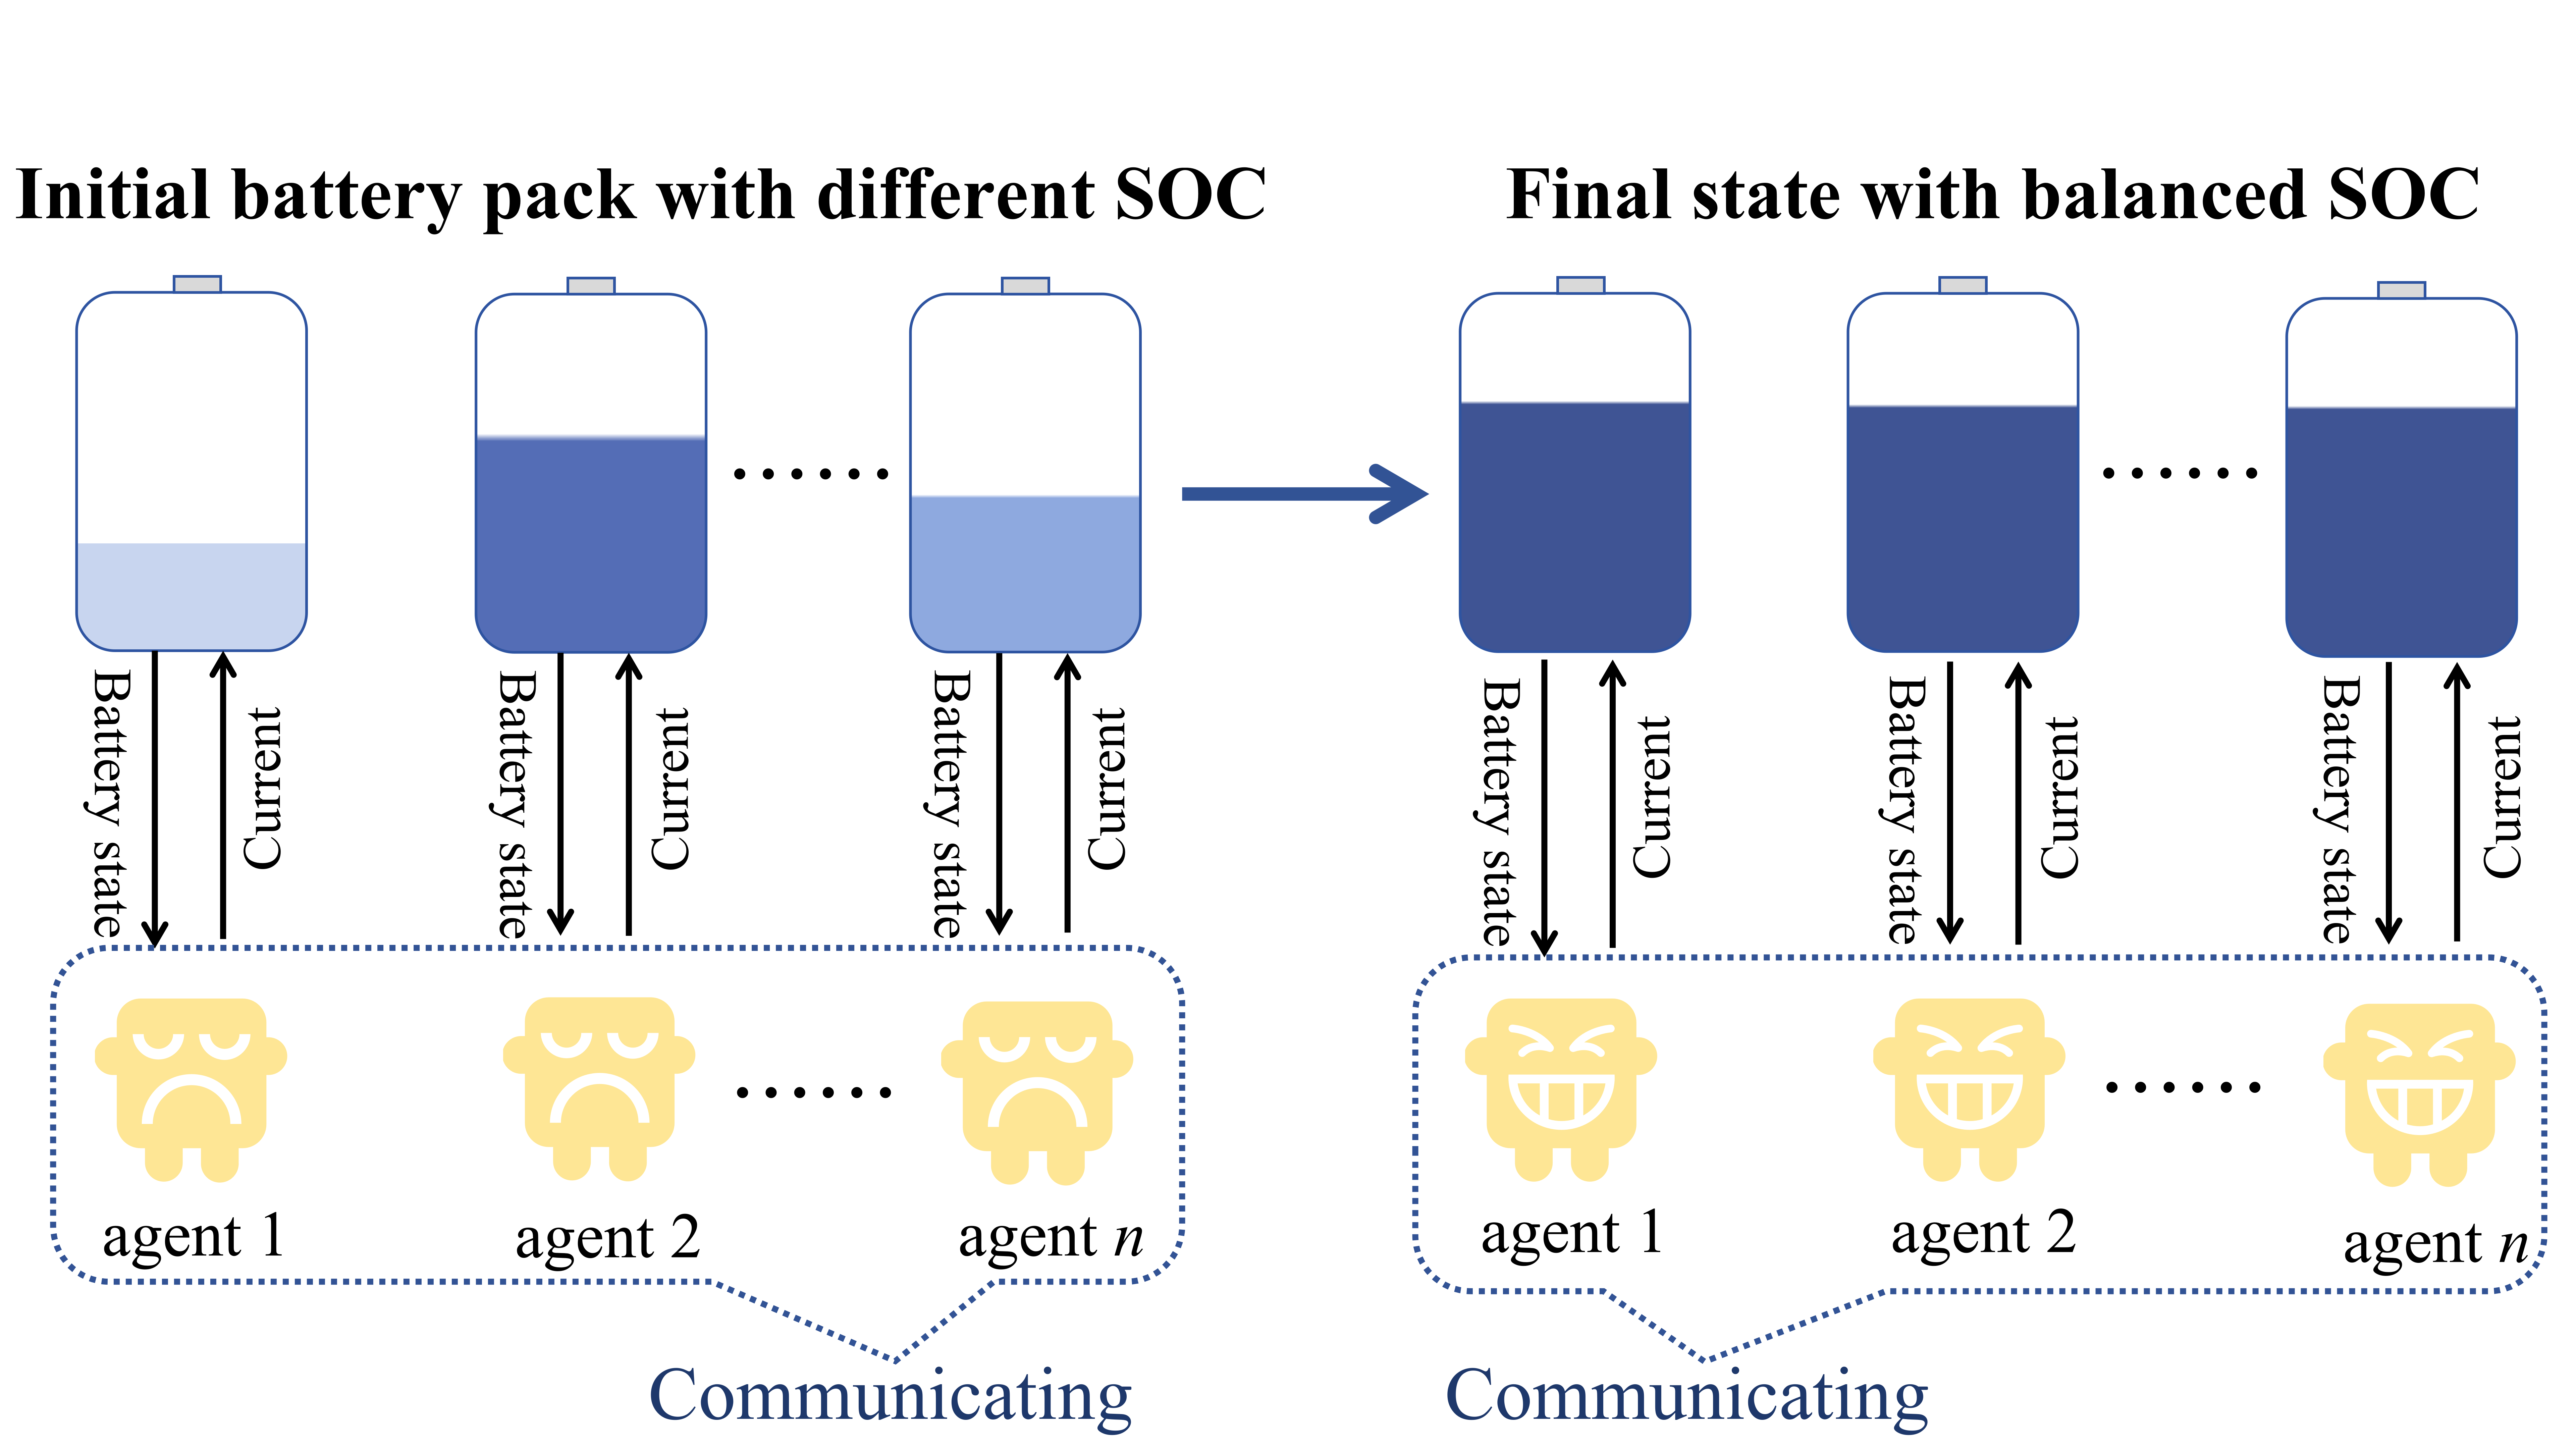
\includegraphics[width=1\linewidth]{marl_control_framework.png}
    \caption{MARL formulation of the battery charging control problem. Each agent regulates the charging current of one cell while sharing the objectives of fast charging and SOC balancing.}
    \label{fig:MARL_Schematic}
\end{figure}

\subsection{MBA-RL Framework}

The MBA-RL architecture is shown in Fig.~\ref{fig:schematic_method}. All agents share one recurrent Q-network. For agent $i$, the network takes the current observation $o_t^i$, the previous executed action $\tilde{a}_{t-1}^i$, and the agent identifier as inputs and estimates the local action value $Q_i$. A mixing network combines the local action values into the joint action value $Q_{\mathrm{tot}}$, with its weights generated by hypernetworks from the global state. Target agent and mixing networks are used to construct the temporal-difference targets during training. \newrev{During execution, the local action values determine the requested currents $\mathbf{a}_t$, and the safety mechanism checks these requests before applying the executed currents $\tilde{\mathbf{a}}_t$ to the cells.}

\begin{figure*}[t]
    \centering
    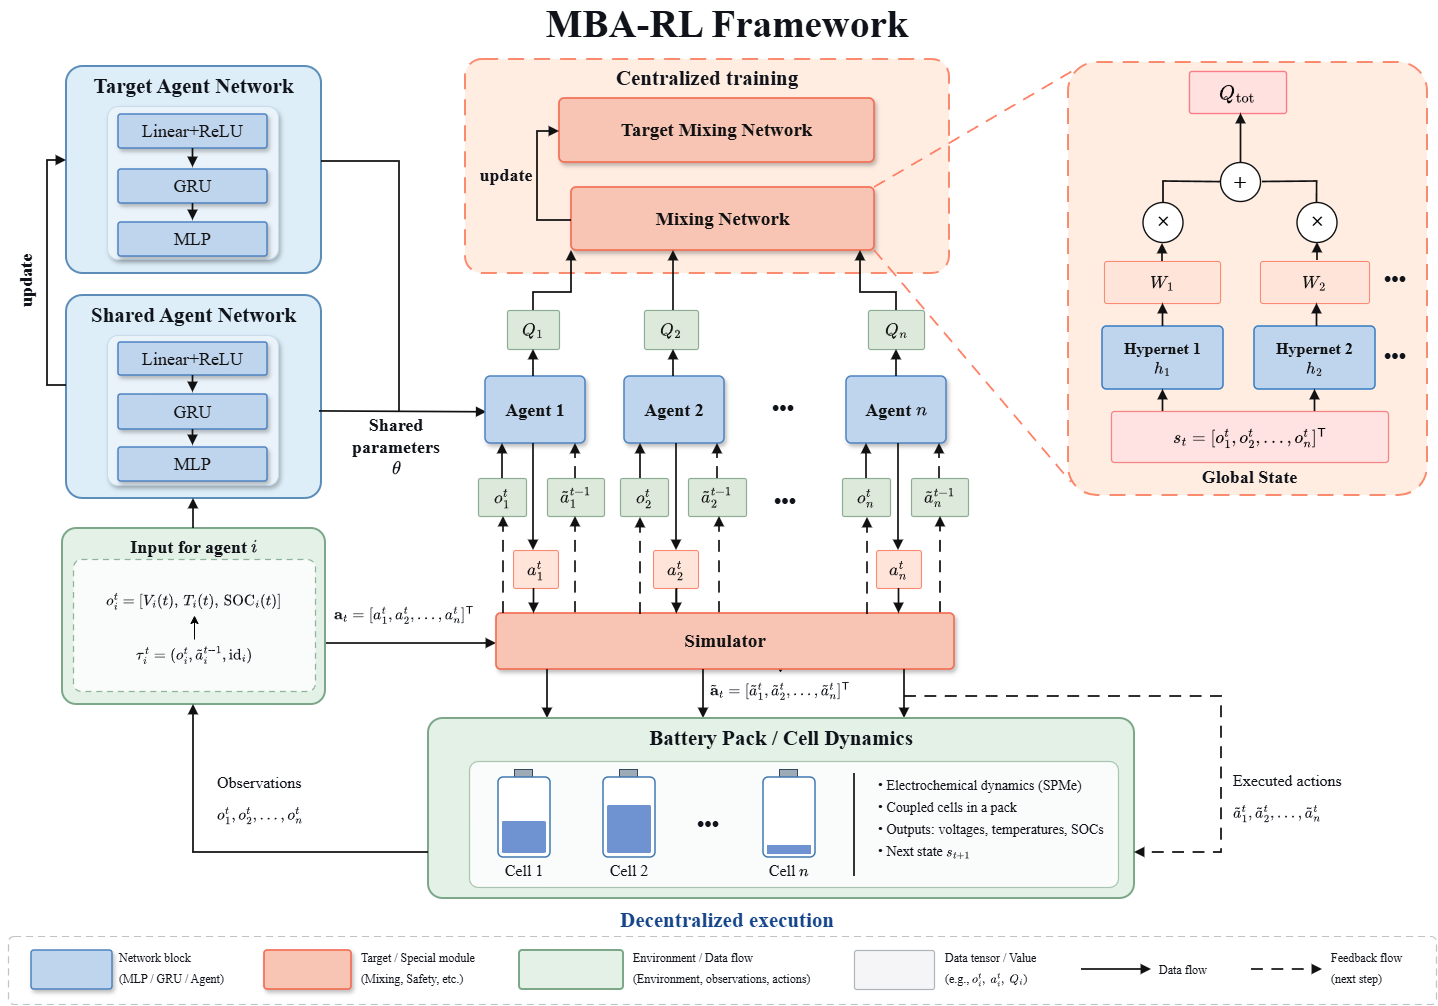
\includegraphics[width=0.9\textwidth,height=\textheight,keepaspectratio]{MBA_RL_Fig2.png}
    \caption{Architecture of the proposed MBA-RL framework. Shared recurrent agents generate cell-level charging currents from local histories, while QMIX enables centralized cooperative value learning. An SPMe-based safety mechanism screens requested currents before execution, and the executed currents are fed back for subsequent decisions.}
    \label{fig:schematic_method}
\end{figure*}

The charging control problem is formulated as a Dec-POMDP \cite{27}:

\[
G=
\left\langle
\mathcal{N},
\mathcal{S},
\{\mathcal{A}_i\}_{i=1}^{n},
\mathcal{P},
\mathcal{R},
\{\mathcal{O}_i\}_{i=1}^{n},
\mathcal{O},
\gamma
\right\rangle .
\]

Here, $\mathcal{N}=\{1,\ldots,n\}$ is the set of agents, $\mathcal{S}$ is the global state space, $\mathcal{A}_i$ and $\mathcal{O}_i$ are the action and observation spaces of agent $i$, $\mathcal{P}$ is the transition kernel, $\mathcal{R}$ is the shared reward function, $\mathcal{O}$ is the observation function, and $\gamma$ is the discount factor.

\subsubsection{State and Observation Spaces}

The global state at time step $t$ is formed by the observations of all cells:

\begin{equation}
\label{eq:global_state}
\mathbf{s}_t
=
\left[
o_t^1,o_t^2,\ldots,o_t^n
\right]^{\mathrm{T}}.
\end{equation}

For agent $i$, the local observation is
$o_t^i=[V_i(t),\allowbreak T_i(t),\allowbreak SOC_i(t)]$, where $V_i(t)$, $T_i(t)$, and $SOC_i(t)$ denote the voltage, temperature, and SOC of cell $i$, respectively. Each agent therefore makes its charging decision from local cell information, while the complete state is available during centralized training.

\subsubsection{Action Space}

Each agent selects a requested charging current from
$\mathcal{A}_{\mathrm{cand}}=\{0,0.5,\ldots,7.5\}\,\mathrm{A}$.
Before action selection, an availability mask removes actions that conflict with the current cell state. When $SOC_i\geq0.95$, only zero current is available. When $V_i\geq V_{\max}$ or $T_i\geq T_{\max}$, currents above 1 A are excluded.

The requested joint action and the corresponding available action space are

\begin{equation}
\label{eq:joint_action}
\mathbf{a}_t
=
\left[
a_t^1,a_t^2,\ldots,a_t^n
\right]^{\mathrm{T}},
\qquad
\mathcal{A}(\mathbf{s}_t)
=
\prod_{i=1}^{n}\mathcal{A}_i(\mathbf{s}_t),
\end{equation}

where $\mathcal{A}_i(\mathbf{s}_t)\subseteq\mathcal{A}_{\mathrm{cand}}$. Let $\mathbf{m}_t$ denote the corresponding availability masks. Since the mask only uses the current state, it does not determine whether a requested current will remain feasible over the next decision interval. The requested current is therefore checked by the model-based safety mechanism before execution.

\subsubsection{Reward Function}

The agents share a reward consisting of a time penalty, an SOC balancing penalty, and penalties for voltage and temperature violations:

\begin{equation}
\label{eq:reward}
r_t
=
r_{\mathrm{time}}
+
r_{\mathrm{bal}}
+
r_{\mathrm{safety}}.
\end{equation}

Before the terminal condition is reached, the time penalty is $r_{\mathrm{time}}=-\lambda_{\mathrm{time}}$. The balancing term is

\begin{equation}
\label{eq:balance_reward}
r_{\mathrm{bal}}
=
\begin{cases}
-\lambda_{\mathrm{bal}}(\sigma-\beta),
& \sigma\geq\beta,\\
0,
& \text{otherwise},
\end{cases}
\end{equation}

where $\sigma$ is the standard deviation of the cell SOCs and $\beta$ is the balancing threshold defined in Section II.

The safety term is
$r_{\mathrm{safety}}=r_{\mathrm{volt}}+r_{\mathrm{temp}}$,
where
$r_{\mathrm{volt}}=\sum_{i=1}^{n}\delta_{v,i}$ and
$r_{\mathrm{temp}}=\sum_{i=1}^{n}\delta_{t,i}$.
The cell-level penalties are defined as

\begin{equation}
\label{eq:safety_reward}
\begin{aligned}
\delta_{v,i}
&=
\begin{cases}
-\lambda_v\left(V_i(t)-V_{\max}\right),
& V_i(t)\geq V_{\max},\\
0,
& \text{otherwise},
\end{cases}
\\[4pt]
\delta_{t,i}
&=
\begin{cases}
-\lambda_T\left(T_i(t)-T_{\max}\right),
& T_i(t)\geq T_{\max},\\
0,
& \text{otherwise}.
\end{cases}
\end{aligned}
\end{equation}

\subsubsection{Transition and Termination}

The current selected by the policy is referred to as the requested current, while the current applied after the safety check is referred to as the executed current. Their joint forms are denoted by $\mathbf{a}_t$ and $\tilde{\mathbf{a}}_t$, respectively.

The transition to the next state is determined by the executed currents and the battery dynamics. The variable $d_t$ indicates whether the episode terminates. Both requested and executed actions are retained during training so that interventions by the safety mechanism are represented explicitly.

\subsection{Cooperative Value Learning}

MBA-RL uses centralized training to coordinate the charging decisions of different cells. Agent $i$ estimates the local action value $Q_i(\tau_t^i,a_t^i|\theta)$ from its action-observation history $\tau_t^i$. During data collection, each agent selects a requested action using an $\epsilon$-greedy policy:

\begin{equation}
\label{epsilon-greedy}
a_t^i =
\begin{cases}
\text{random available action},
& \text{with probability }\epsilon,\\
\displaystyle
\arg\max_{a_t^i}
Q_i(\tau_t^i,a_t^i|\theta),
& \text{with probability }1-\epsilon.
\end{cases}
\end{equation}

All agents share the same network parameters $\theta$. A one-hot agent identifier is included in the network input so that the shared network can distinguish among cells.

The mixing network combines the local action values into the joint action value

\begin{equation}
\label{Q-value}
Q_{\mathrm{tot}}
(\boldsymbol{\tau}_t,\mathbf{a}_t|\phi)
=
f\left(
Q_1(\tau_t^1,a_t^1|\theta),
\ldots,
Q_n(\tau_t^n,a_t^n|\theta)
\right),
\end{equation}

where $\boldsymbol{\tau}_t$ denotes the joint action-observation history and $\phi$ denotes the parameters of the mixing network.

QMIX imposes the monotonicity constraint

\begin{equation}
\label{QMIX_constraints}
\frac{\partial Q_{\mathrm{tot}}}{\partial Q_i}
\geq 0,
\qquad
i=1,2,\ldots,n.
\end{equation}

This constraint makes decentralized greedy action selection consistent with maximizing the joint action value, allowing each agent to select its action independently during execution.

The target agent and mixing networks are synchronized with their online counterparts every $N_t$ training episodes. Considering the terminal flag and the available actions at the next state, the target value is

\begin{equation}
\label{target Q}
y_t^{\mathrm{tot}}
=
r_t
+
\gamma(1-d_t)
\max_{\mathbf{a}_{t+1}\in\mathcal{A}(\mathbf{s}_{t+1})}
Q_{\mathrm{tot}}
(
\boldsymbol{\tau}_{t+1},
\mathbf{a}_{t+1}
|\phi'
).
\end{equation}

The shared reward couples the local charging decisions through $Q_{\mathrm{tot}}$. The time penalty encourages faster charging, while the balancing term penalizes SOC differences among cells. The agents are therefore trained to coordinate their charging currents toward the common objectives of fast charging and SOC balancing.

\subsection{Model-Based Safety Mechanism}

At each decision step, MBA-RL first generates a requested current for each cell. Starting from this value, the safety mechanism evaluates the requested current and successively lower candidates using the nominal SPMe over the next decision interval, followed by an interval with zero current.

\begin{table}[!t]
\centering
\caption{Control and evaluation settings}
\label{tab:experimental_settings}
\scriptsize
\setlength{\tabcolsep}{3pt}
\begin{tabular}{@{}p{0.31\columnwidth}p{0.63\columnwidth}@{}}
\toprule
Setting & Value \\
\midrule
Battery model & SPMe with lumped thermal model \\
Current command & $0$--$7.5$ A, 0.5 A step, 90 s interval \\
Task criterion & $SOC_i\geq0.90$, $\sigma\leq0.02$, 5400 s horizon, 270 s hold \\
Operating limits & $V\leq4.2$ V, $T\leq309$ K, $SOC\leq0.95$ \\
Safety margins & 0.03 V and 1 K \\
Ambient temperature & 298.15 K \\
\bottomrule
\end{tabular}
\end{table}

\newrev{Let $\widehat{V}_{i,t}^{\mathrm{pk}}(u)$, $\widehat{T}_{i,t}^{\mathrm{pk}}(u)$, and $\widehat{SOC}_{i,t}^{\mathrm{pk}}(u)$ denote the nominal peaks over the candidate-current interval and the following zero-current interval. The observation-model discrepancies define the corrections $b_{V,i,t}=\max\{V_i(t)-\widehat{V}_i(t),0\}$, $b_{T,i,t}=\max\{T_i(t)-\widehat{T}_i(t),0\}$, and $b_{SOC,i,t}=|SOC_i(t)-\widehat{SOC}_i(t)|$. The feasible candidate set is}

\begin{equation}
\label{eq:safety_candidates}
\newrev{\begin{gathered}
\mathcal{F}_{i,t}=\bigl\{u\in\mathcal{A}_{\mathrm{cand}}:\;0\leq u\leq a_t^i,\\[-1pt]
\begin{aligned}
\widehat{V}_{i,t}^{\mathrm{pk}}(u)+b_{V,i,t}&\leq V_{\max}-\delta_V,\\[-1pt]
\widehat{T}_{i,t}^{\mathrm{pk}}(u)+b_{T,i,t}&\leq T_{\max}-\delta_T,\\[-1pt]
\widehat{SOC}_{i,t}^{\mathrm{pk}}(u)+b_{SOC,i,t}&\leq SOC_{\max}\bigr\}.
\end{aligned}
\end{gathered}}
\end{equation}

\newrev{Here, $\delta_V$ and $\delta_T$ are the safety margins in Table~\ref{tab:experimental_settings}. The executed current is $\tilde{a}_t^i=\max\mathcal{F}_{i,t}$ whenever this set is nonempty. The peak constraints are checked at the model sampling points over the two prediction intervals, and candidates with unsuccessful model predictions are excluded.}

If no feasible current is found for any cell, the episode terminates without advancing the battery model. The same safety mechanism is used during training and testing. In this way, requested currents are checked over the prediction interval before they are executed.

\subsection{Training Procedure}

Complete episodes are stored in the replay buffer $\mathcal{D}$. Each transition contains the state, availability mask, requested action, executed action, reward, next state, next availability mask, and terminal flag. During training, batches of complete episodes are sampled from the replay buffer.

The Q-function is evaluated using the requested action selected by the policy, while the executed action is included in the subsequent action-observation history. This allows the agent network to account for modifications made by the safety mechanism. \newrev{After training, the learned network parameters are held fixed and the agents select the available actions greedily during evaluation; the same safety mechanism remains active.}

The training hyperparameters are summarized in Table~\ref{tab:training_settings}, and the overall procedure is given in Algorithm~\ref{alg:QMIX}. In Algorithm~\ref{alg:QMIX}, $\bm{\theta}$ denotes the mixing-network parameters $\phi$.

\begin{table}[!t]
\centering
\caption{Training implementation settings}
\label{tab:training_settings}
\scriptsize
\setlength{\tabcolsep}{3pt}
\renewcommand{\arraystretch}{1.03}
\begin{tabular}{@{}p{0.38\columnwidth}p{0.56\columnwidth}@{}}
\toprule
\textbf{Setting} & \textbf{Value} \\
\midrule
Training horizon & 2500 steps \\
Replay buffer / batch size & 800 episodes / 32 episodes \\
Learning rate & $2\times10^{-4}$ \\
Target-network update & Every 50 episodes \\
Exploration schedule & $0.5\rightarrow0.05$ over the first 80\% of training \\
Reward weights & $\lambda_{\mathrm{time}}=0.75$, $\lambda_{\mathrm{bal}}=50$, $\lambda_v=20$, $\lambda_T=2$ \\
Network widths & Agent/mixer/hypernetwork: 128/256/64 \\
\bottomrule
\end{tabular}
\end{table}

\begin{algorithm}[t]
    \caption{MBA-RL charging control framework}
    \label{alg:QMIX}

    \begin{algorithmic}[1]
        \STATE Initialize $\theta, \theta', \bm{\theta}, \bm{\theta}'$ randomly
        \STATE Set the learning rate $\alpha$, number of episodes $N_{episode}$, and replay buffer $\mathcal{D}$
        \STATE $\theta' \leftarrow \theta, \bm{\theta}' \leftarrow \bm{\theta}$
        \FOR{$episode =$ 1 to $N_{episode}$}
            \STATE $t\leftarrow 0$, $\tau_t^i \leftarrow \emptyset$, and observe the initial state $\mathbf{s}_t$

            // \textbf{Data Collection}
            \WHILE{$\neg done$}
                \FOR{the $i$-th agent}
                    \STATE $\tau_t^i \leftarrow \tau_{t-1}^i \cup \{(o_t^i, a_{t-1}^i)\}$
                    \STATE $\epsilon \gets 0.5 (1 - \frac{episode}{N_{episode}})$
                    \STATE Select $a_t^i$ according to \eqref{epsilon-greedy}
                \ENDFOR
                \STATE Execute the joint action $\mathbf{a}_t$, observe the reward $r_t$, and get the next state $\mathbf{s}_{t+1}$
                \STATE $\mathcal{D} \leftarrow \mathcal{D} \cup \{ \langle\mathbf{s}_t, \mathbf{a}_t, r_t, \mathbf{s}_{t+1}, done\rangle \}$
            \ENDWHILE

            // \textbf{Network Update}
            \IF{$|\mathcal{D}| > N$}
                \STATE $B \leftarrow$ Randomly sample data from $N$ episodes in $\mathcal{D}$
                \FOR{each time step $t$ in each episode in batch $B$}
                    \STATE Calculate $Q_{tot}$ by \eqref{Q-value} based on the state $\mathbf{s}_t$
                    \STATE Calculate $y^{\text{tot}}$ by \eqref{target Q} based on the state $\mathbf{s}_{t+1}$
                \ENDFOR
                \STATE Under the monotonicity condition given in \eqref{QMIX_constraints}, utilize the RMSprop  optimizer \cite{zou2019sufficient} to update $\theta$ and $\bm{\theta}$ by minimizing the loss function: $\left( y_{\text{tot}} - Q_{\text{tot}} \right)^2$
            \ENDIF
            \IF{$episode$ \% $N_t$ == 0}
                \STATE $\theta' \leftarrow \theta$, $\bm{\theta}' \leftarrow \bm{\theta}$
            \ENDIF
        \ENDFOR
    \end{algorithmic}
\end{algorithm}
% End merged section: 03_method.tex

% Begin merged section: 04_results.tex
\section{Results and Discussion}

The performance of MBA-RL was evaluated using cell-specific models identified from three Samsung 40T 21700 cells, denoted as Cell 1, Cell 2, and Cell 3. Each cell has a nominal capacity of 4000 mAh and a maximum discharge current of 35 A. Voltage and temperature measurements were collected using the NEWARE CT-4008-5V20A-A platform shown in Fig.~\ref{fig:experiment_Schematic}. These measurements were used for parameter identification, after which the identified SPMe models were used for simulation-based policy training and evaluation with independently controlled charging currents.

\begin{figure}[!t]
\centering
\includegraphics[width=0.95\columnwidth]{experimental_platform.png}
\caption{Experimental platform}
\label{fig:experiment_Schematic}
\end{figure}

\subsection{Parameter Identification for Cells with Different Cycling Histories}

To introduce differences in cycling history, Cells 2 and 3 were subjected to 140 and 260 charge-discharge cycles, respectively. The voltage and temperature measurements in Fig.~\ref{fig:three_aging} were used to identify the SPMe parameters of each cell using PSO \cite{28}.

\begin{figure}[!t]
\centering
\begin{minipage}[t]{0.48\columnwidth}
\centering
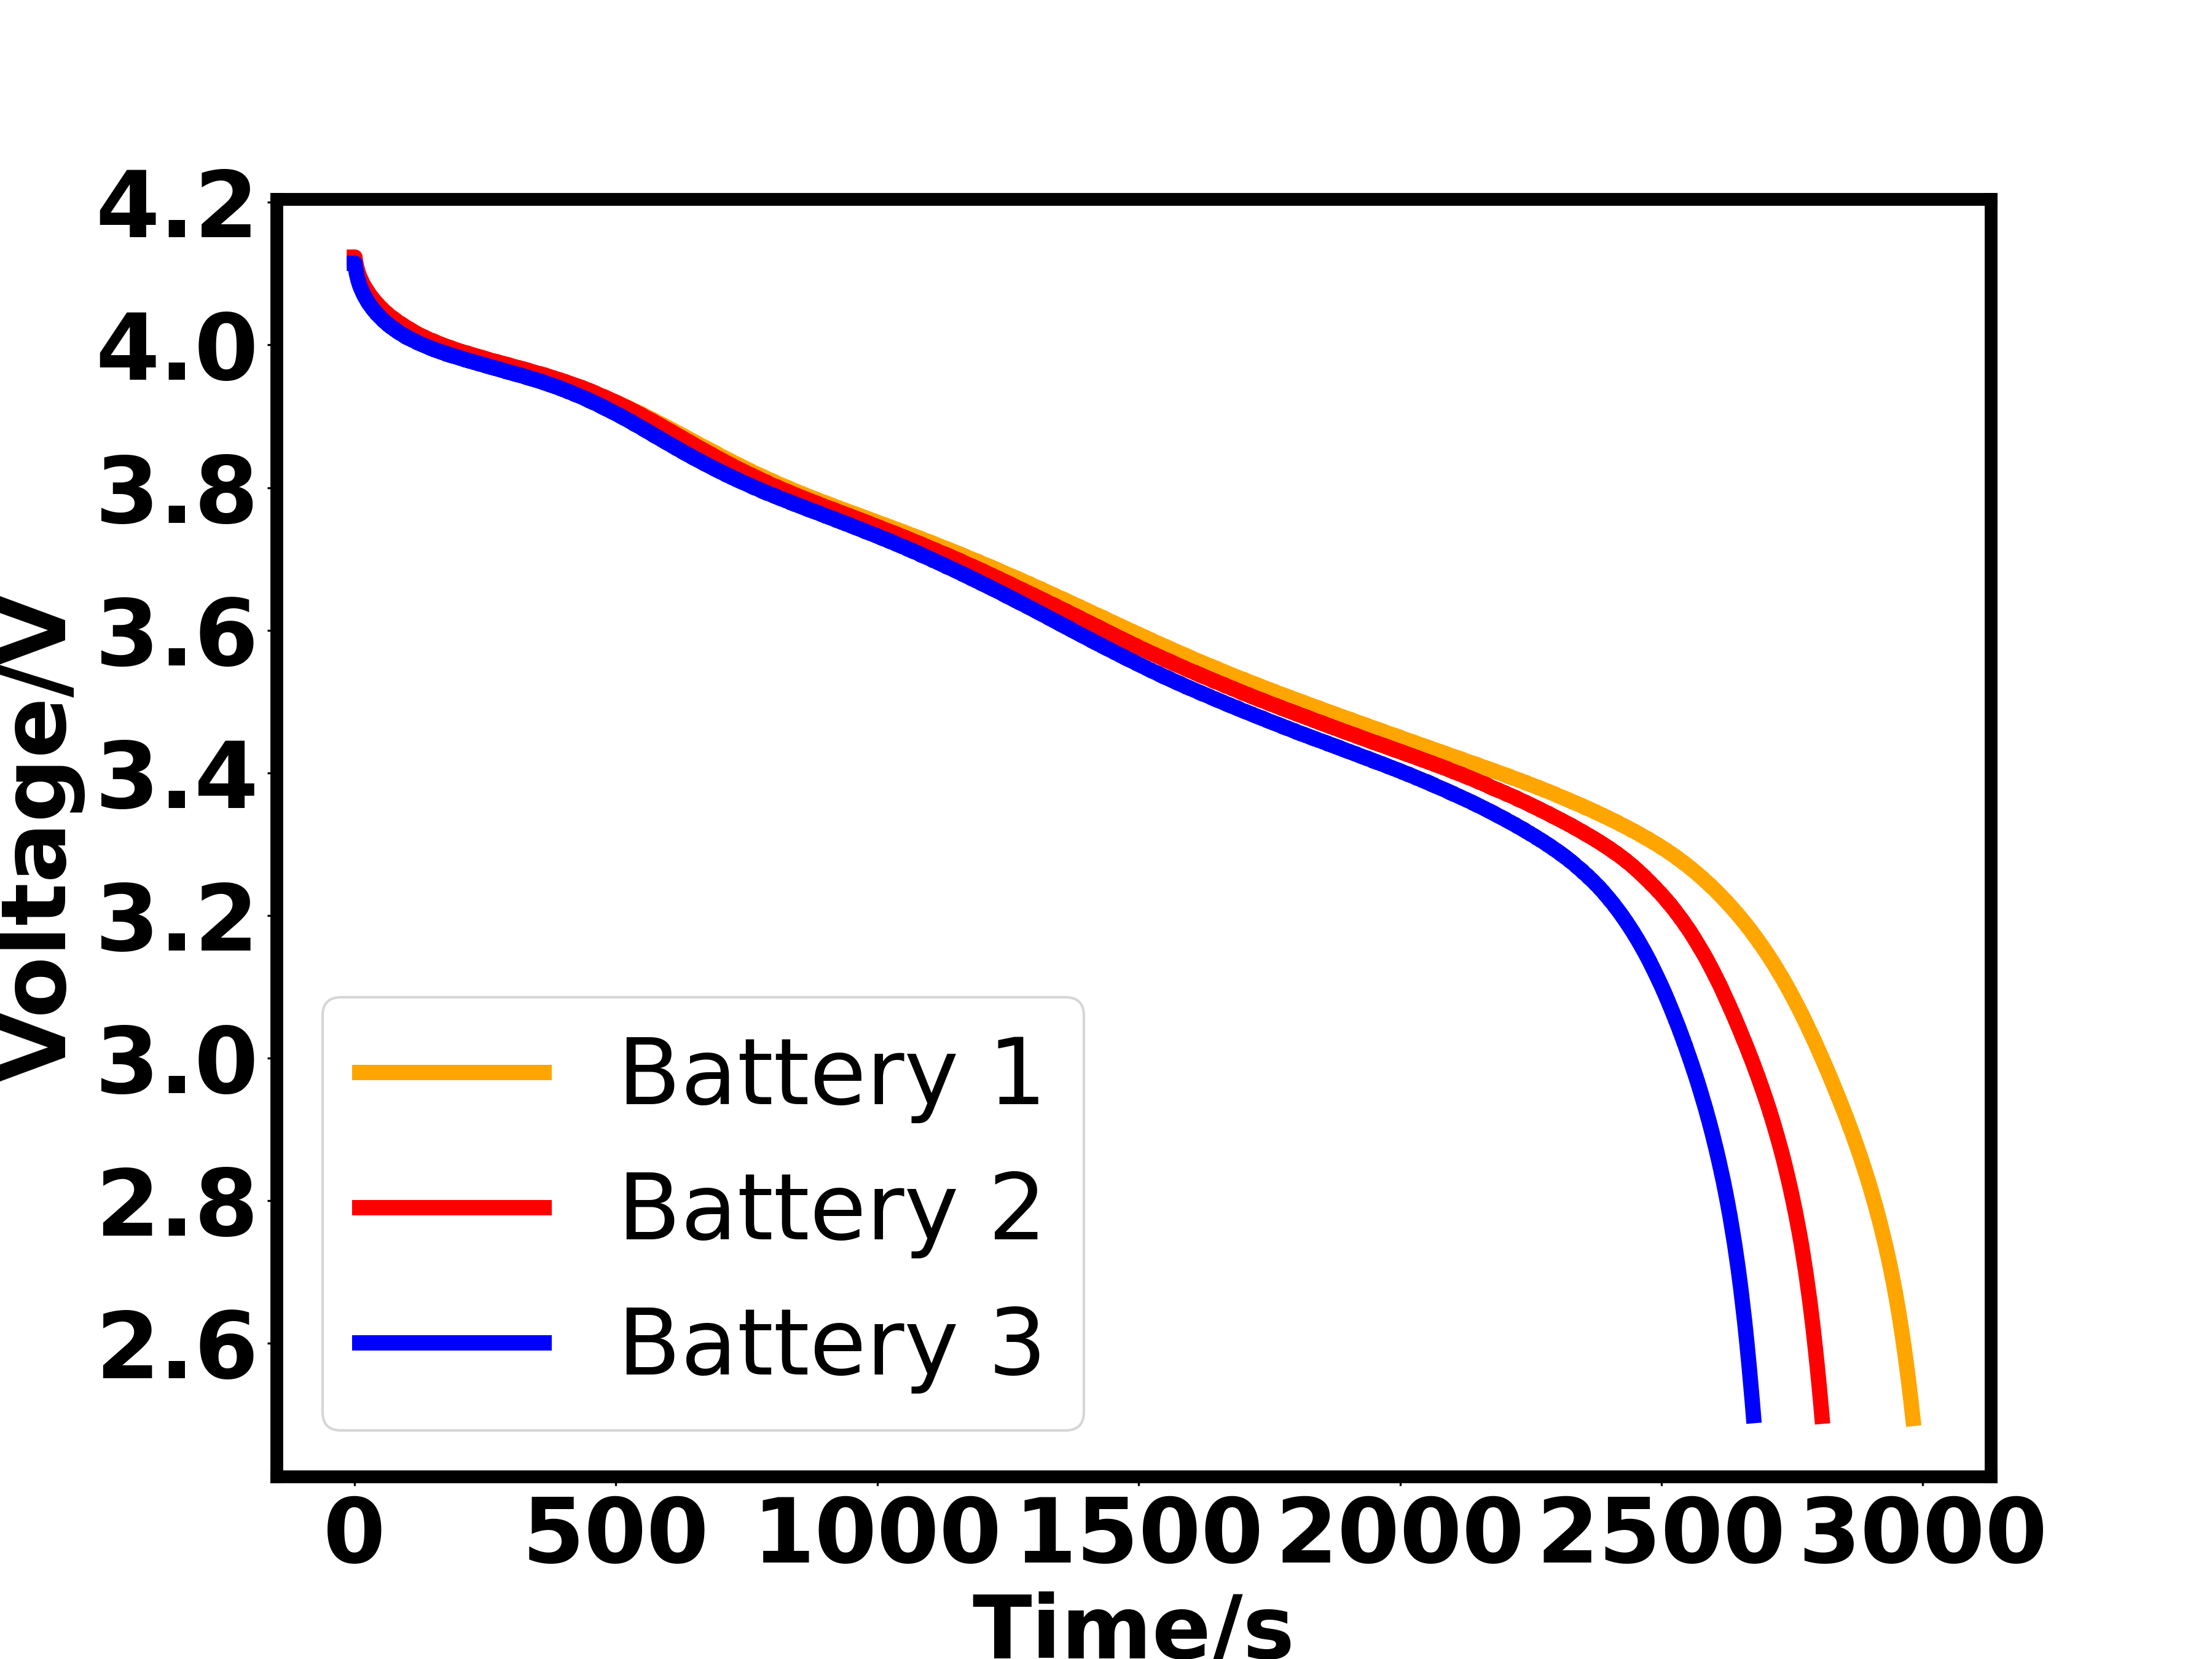
\includegraphics[width=\linewidth]{aging_voltage.png}
\end{minipage}
\begin{minipage}[t]{0.48\columnwidth}
\centering
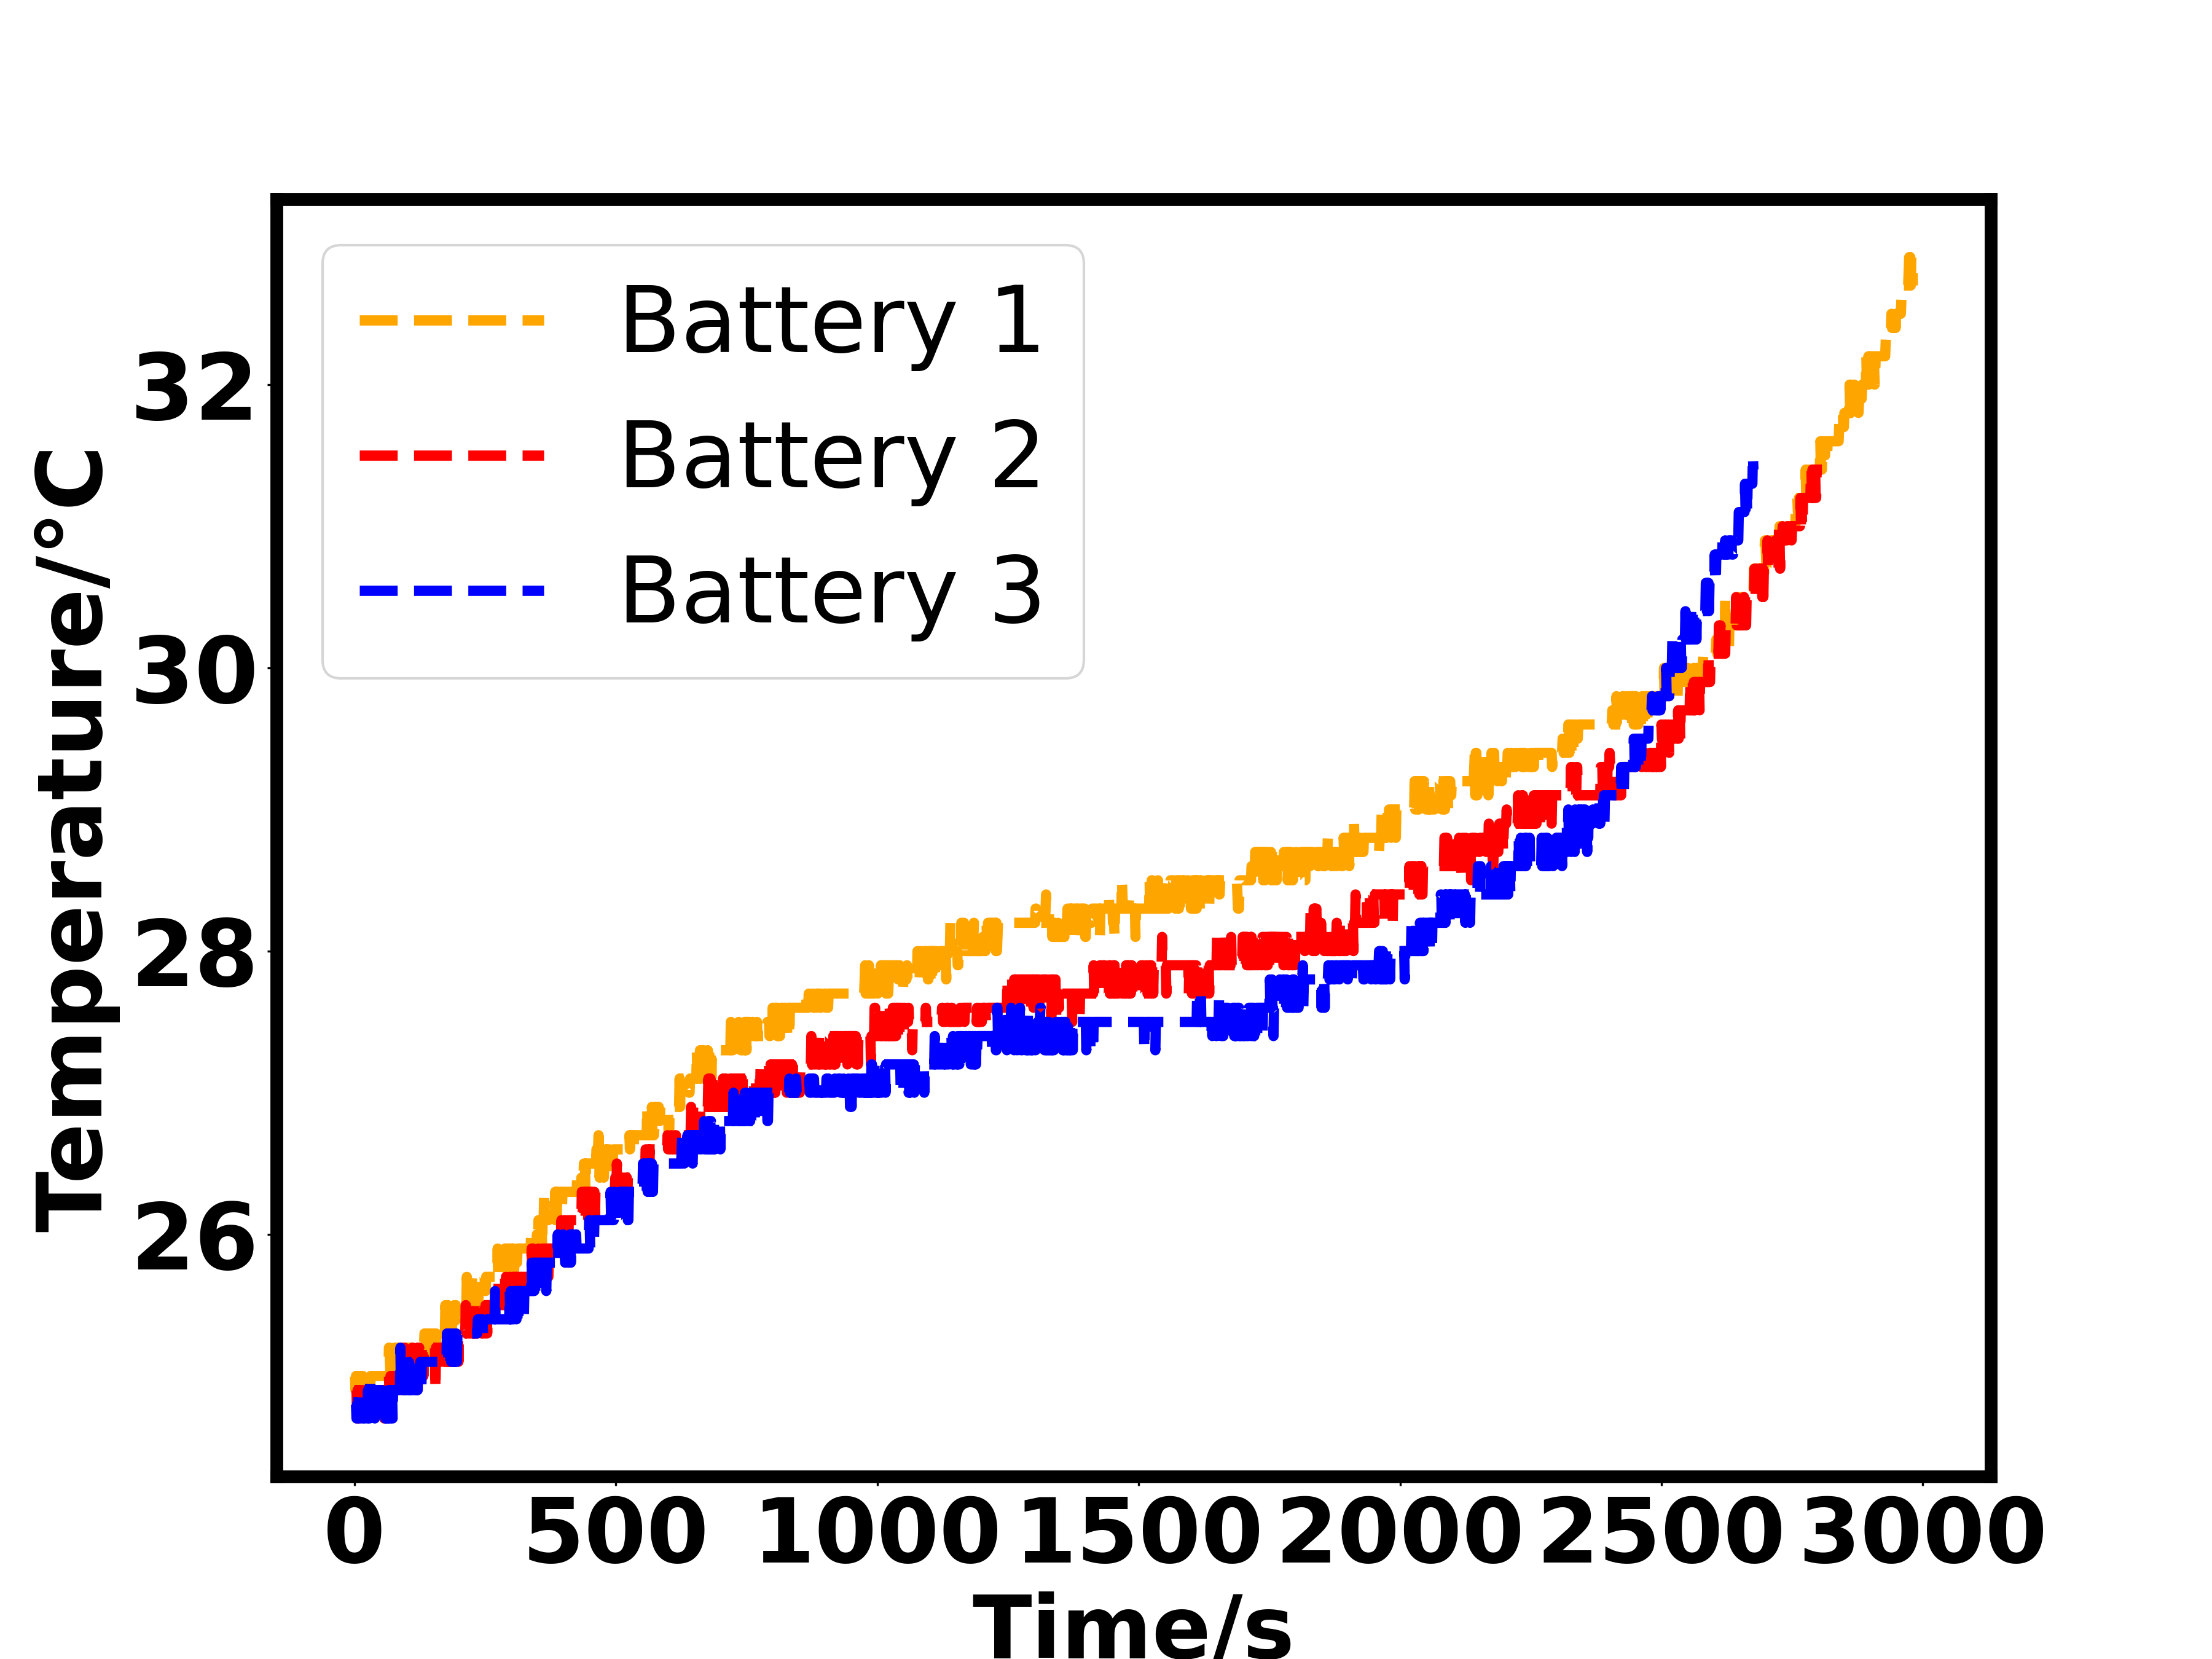
\includegraphics[width=\linewidth]{aging_temperature.png}
\end{minipage}
\caption{Voltage and temperature measurements under different cycling histories}
\label{fig:three_aging}
\end{figure}

Fig.~\ref{fig:cell_validation} compares the identified-model outputs with the corresponding measurements. The RMSE values in Table~\ref{tab:cell_rmse} indicate that the models reproduce the measured voltage and temperature profiles under the identification conditions.

\begin{figure}[!t]
\centering
\subfloat[Cell 1 voltage]{%
\begin{minipage}[t]{0.48\columnwidth}
\centering
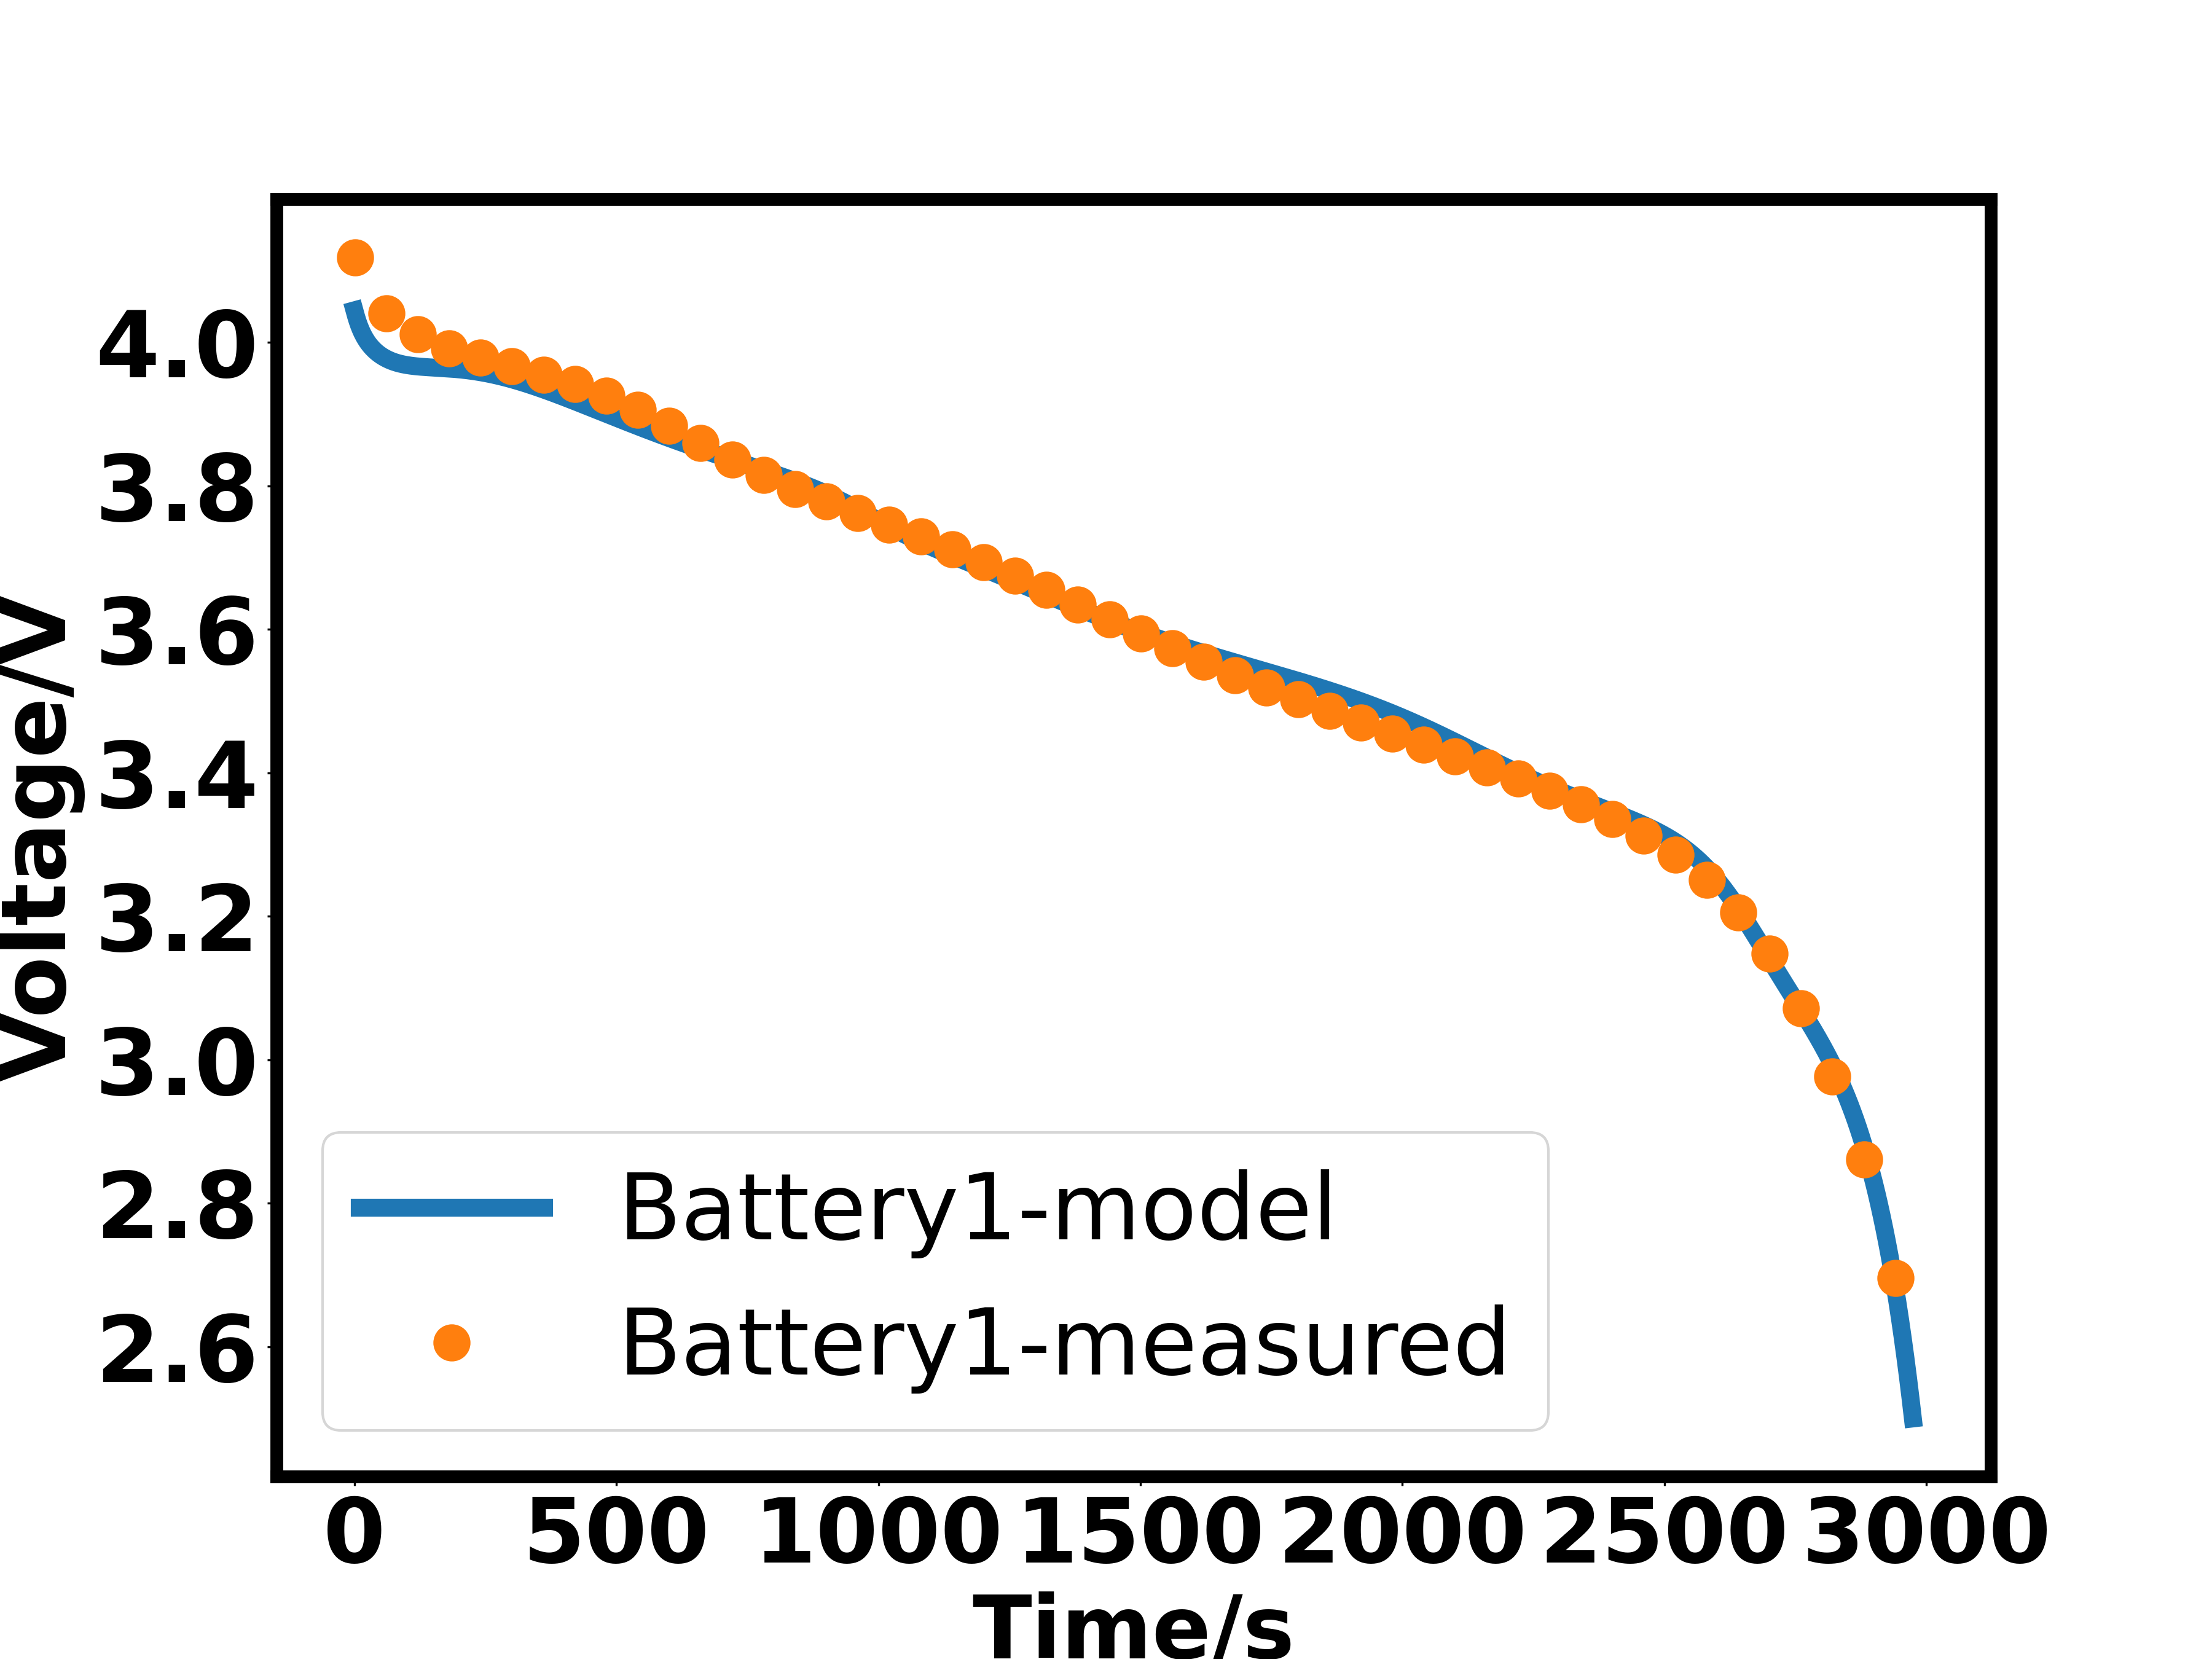
\includegraphics[width=\linewidth]{cell1_voltage_fit.png}
\end{minipage}%
}\hfill
\subfloat[Cell 1 temperature]{%
\begin{minipage}[t]{0.48\columnwidth}
\centering
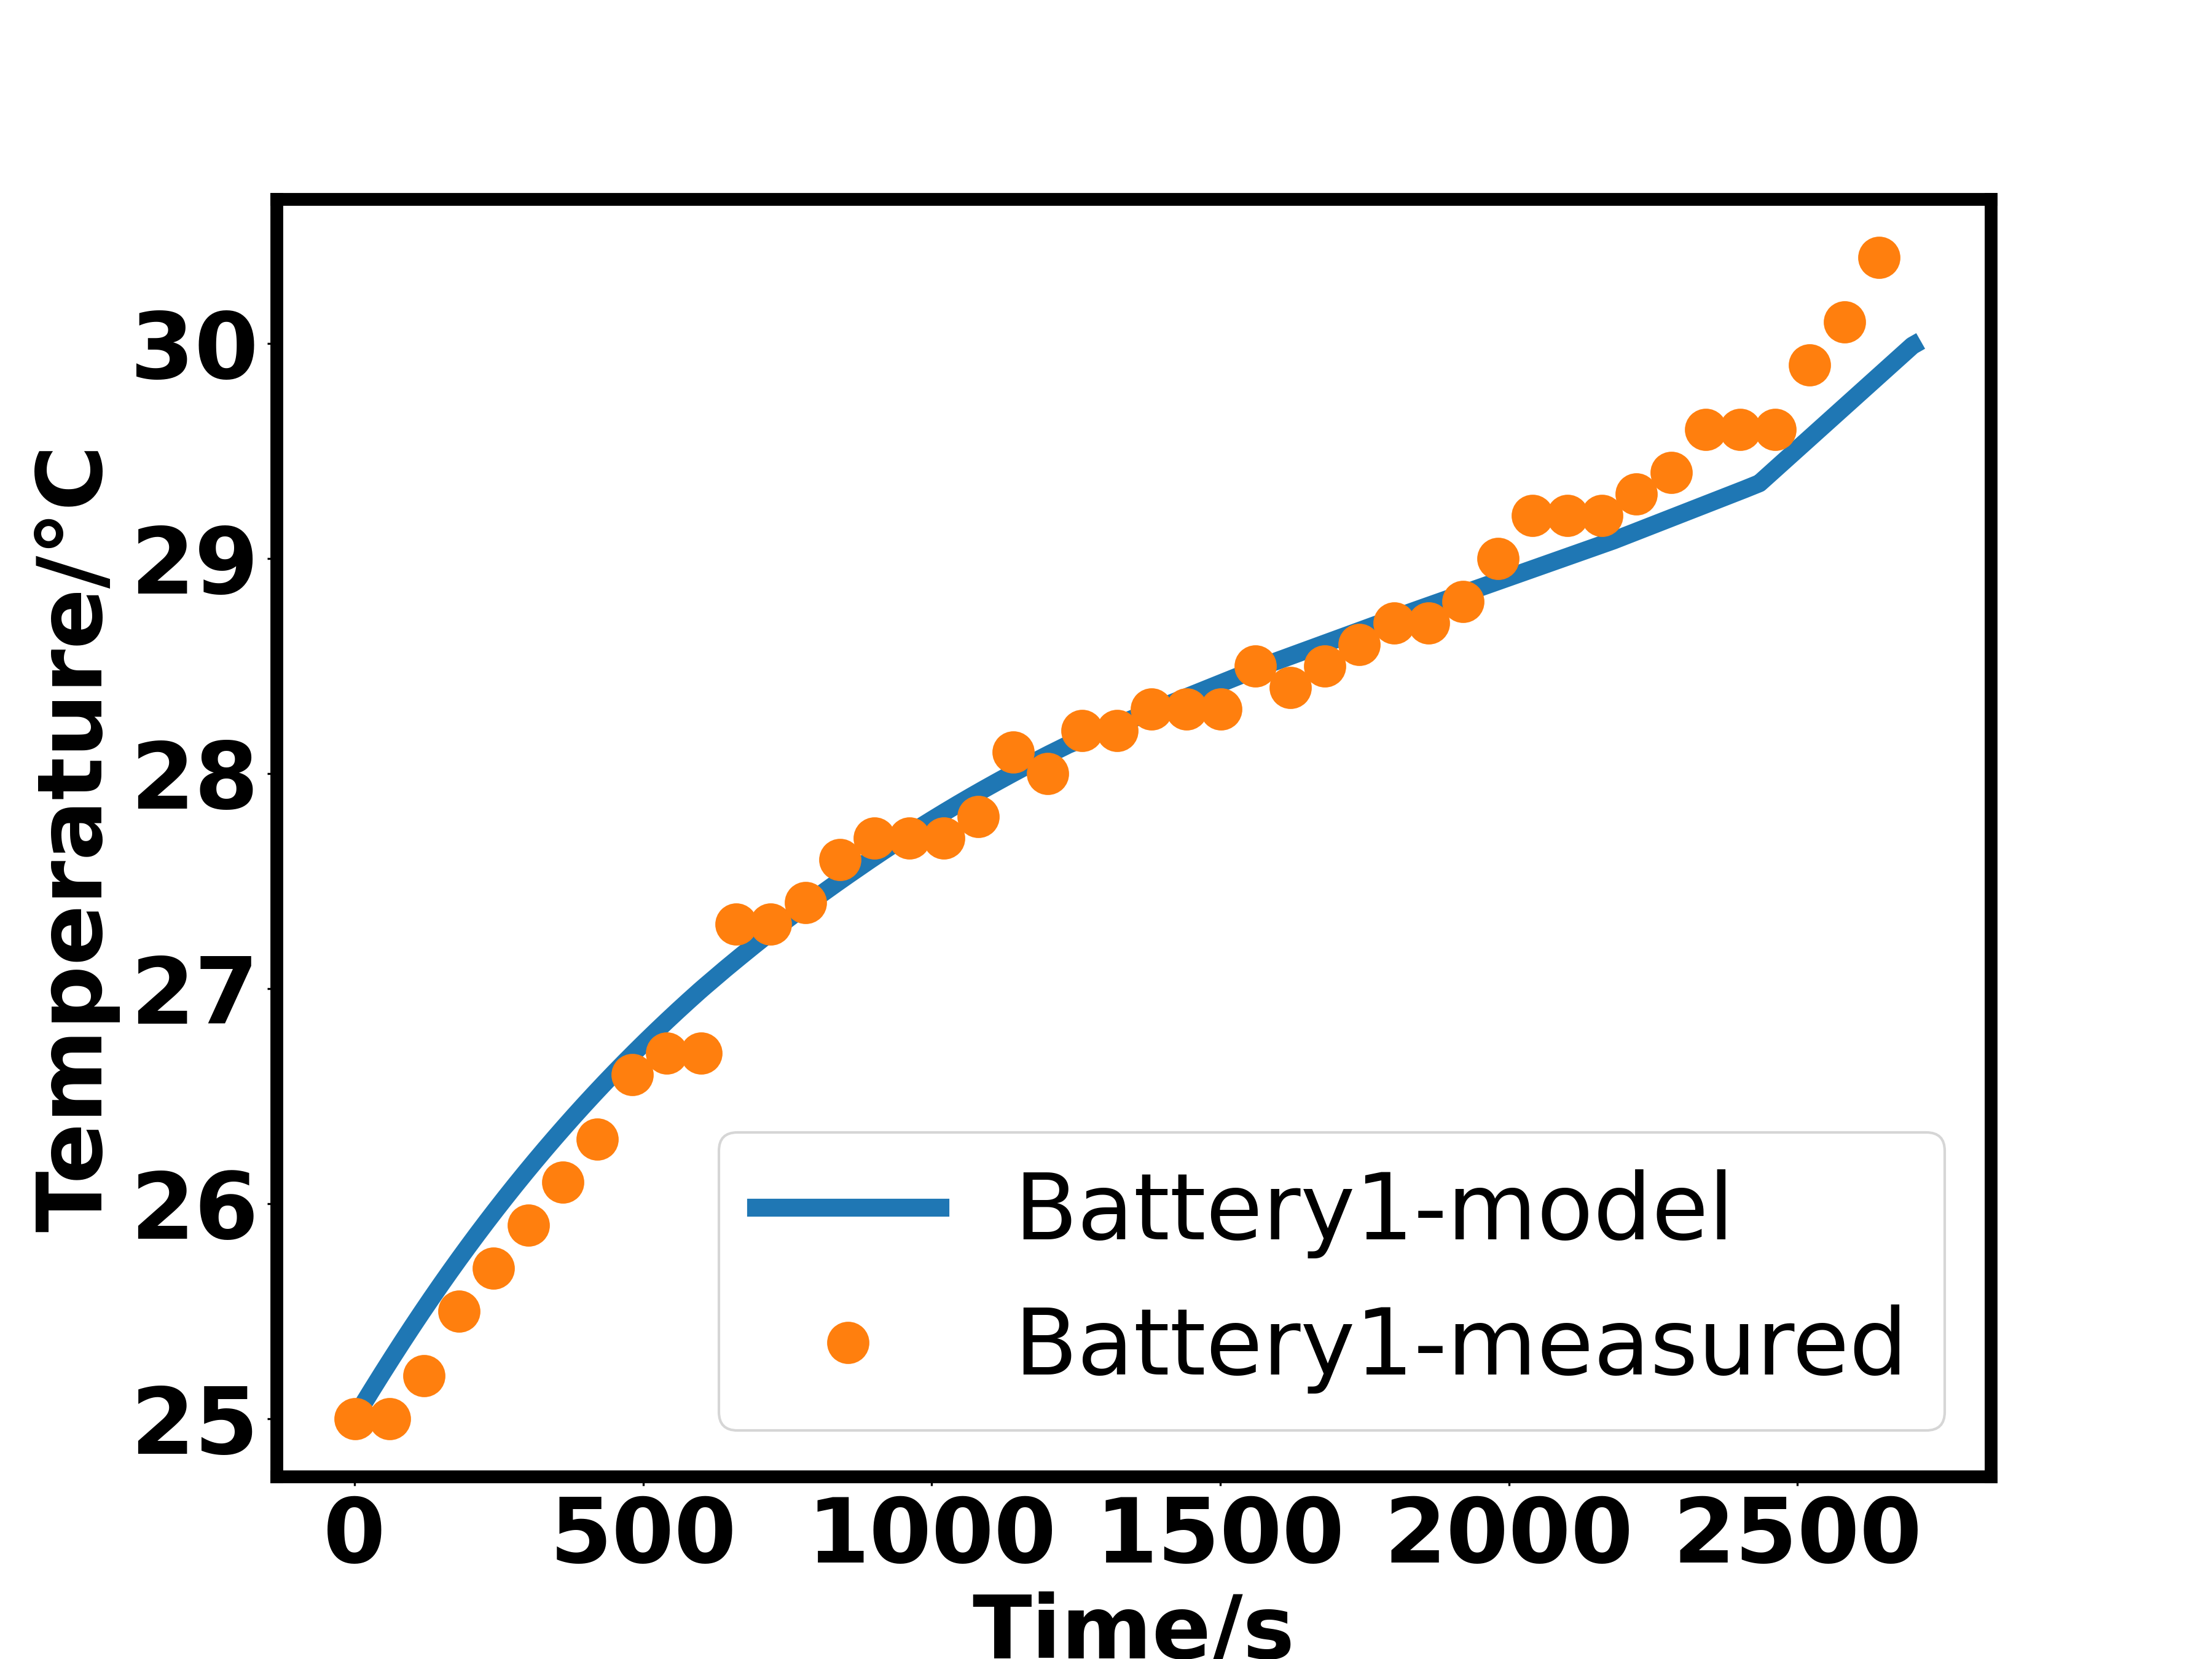
\includegraphics[width=\linewidth]{cell1_temperature_fit.png}
\end{minipage}%
}\par\smallskip
\subfloat[Cell 2 voltage]{%
\begin{minipage}[t]{0.48\columnwidth}
\centering
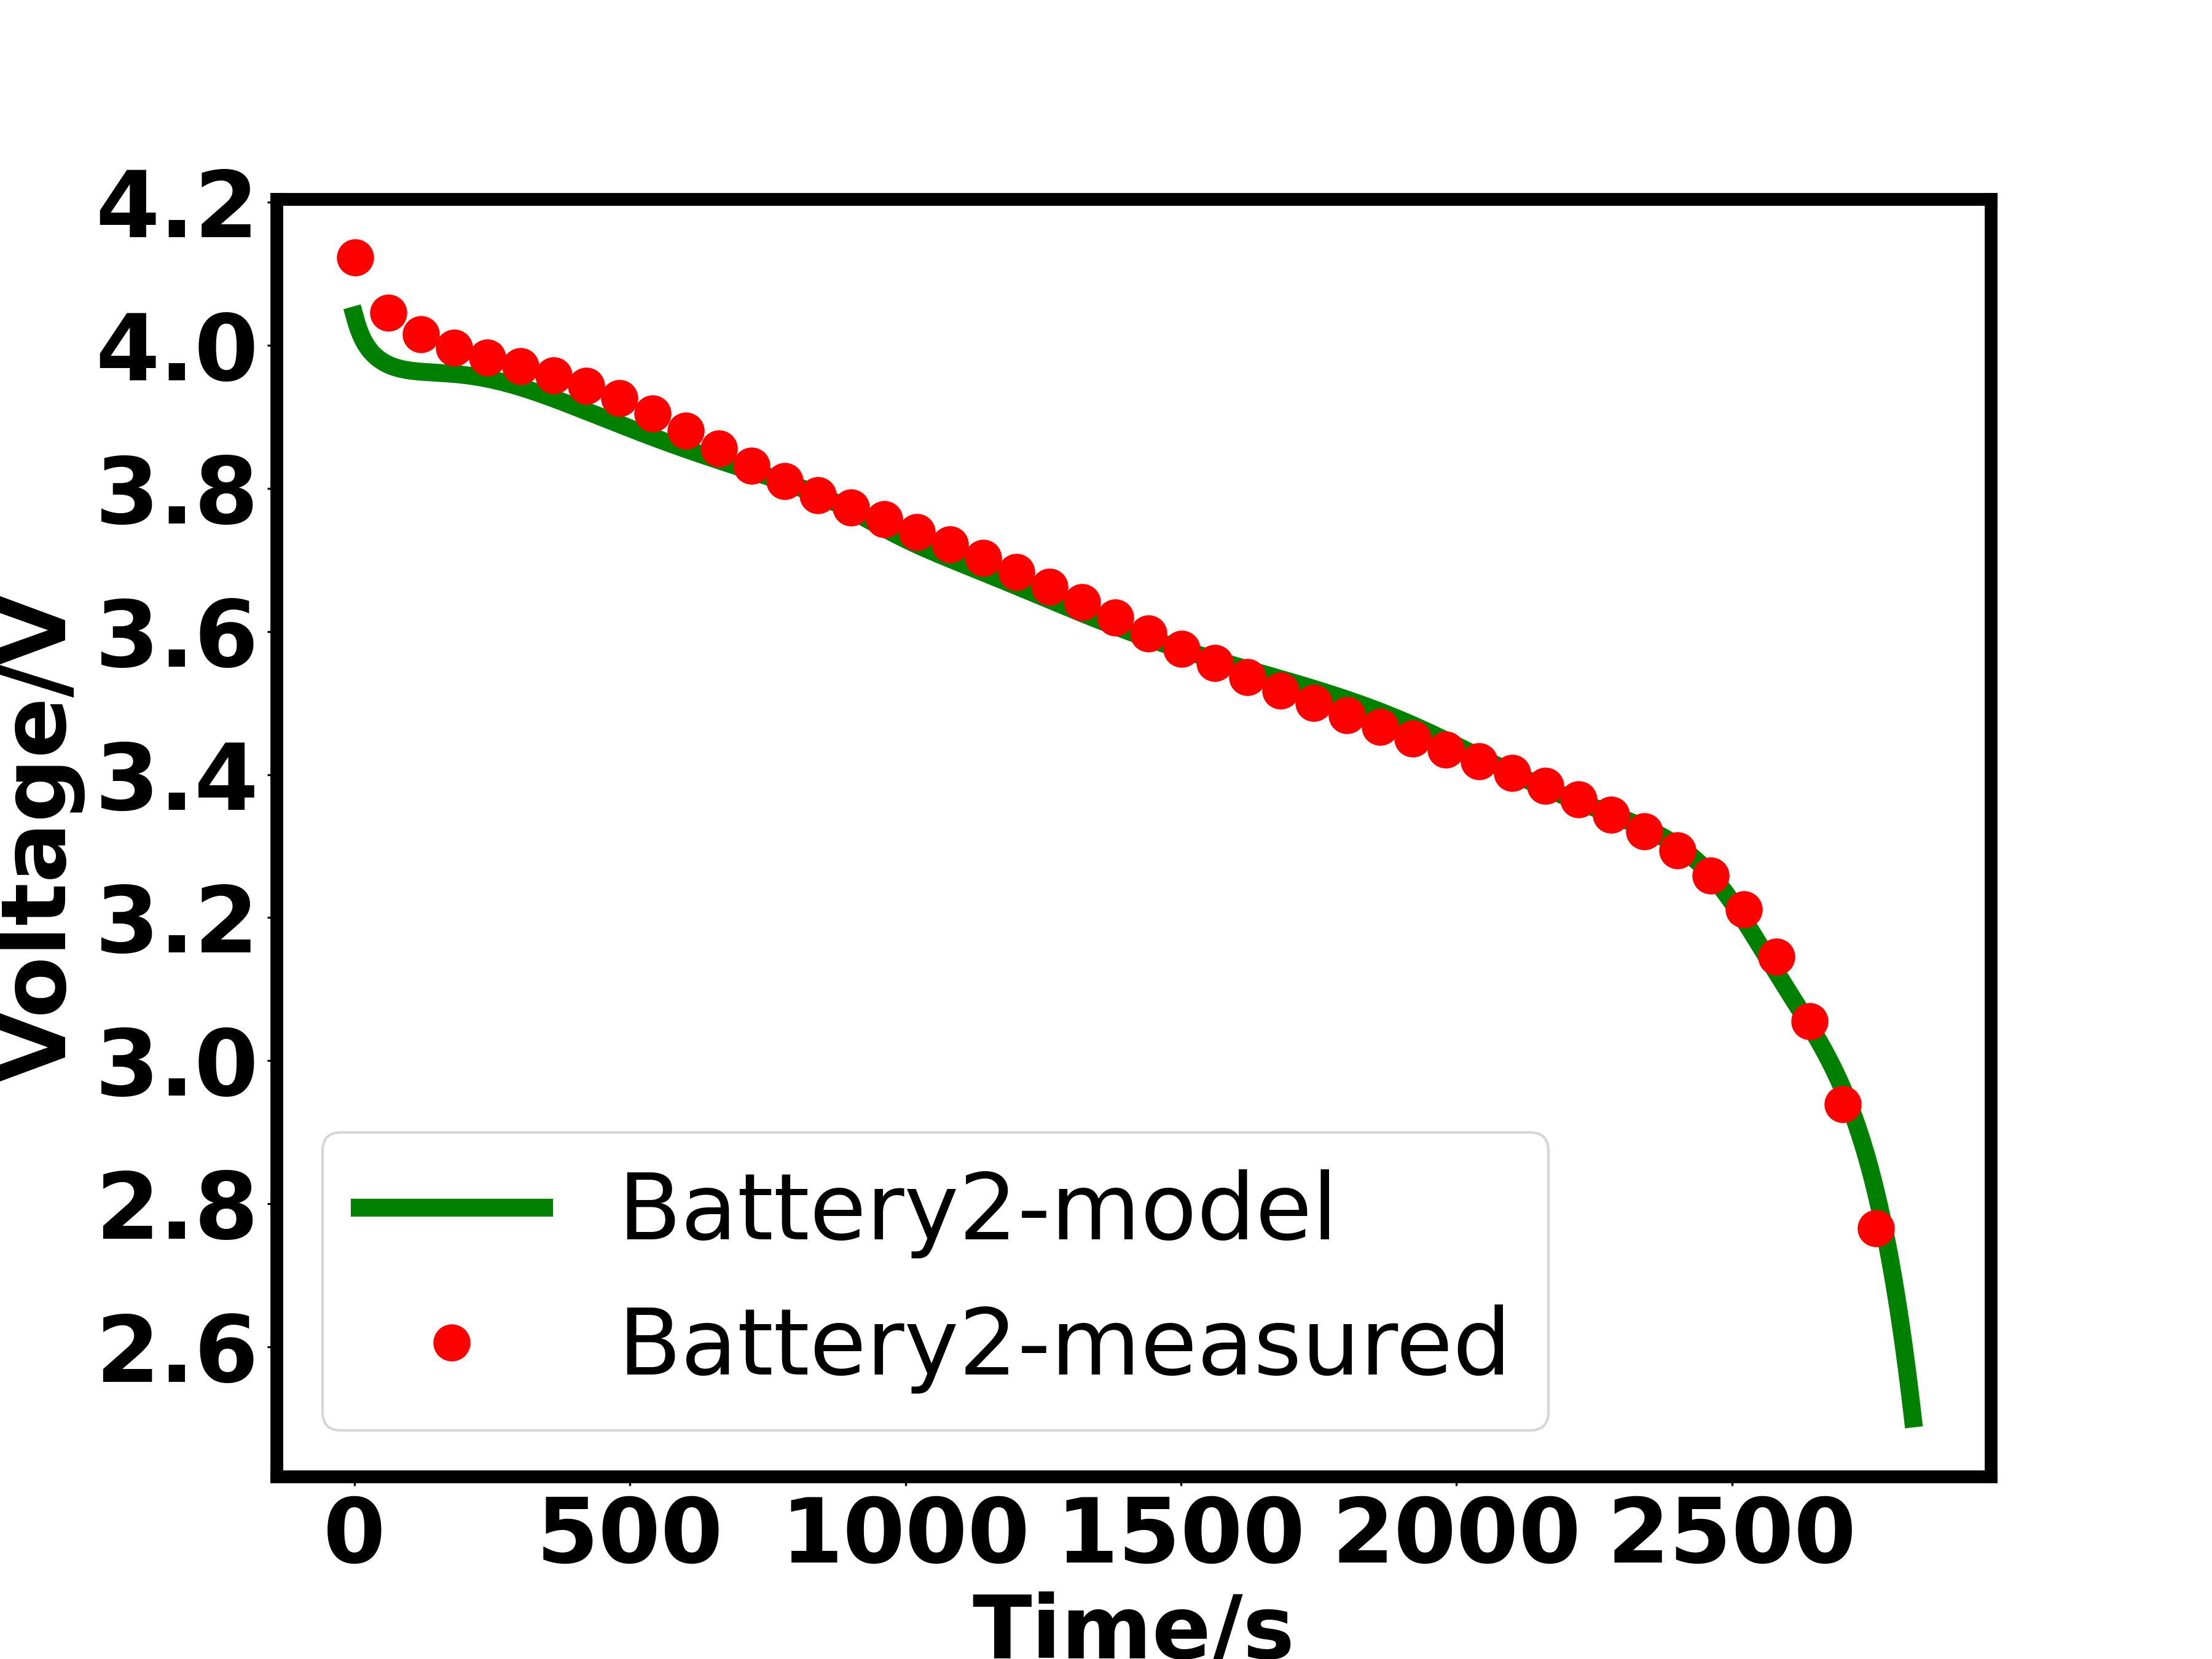
\includegraphics[width=\linewidth]{cell2_voltage_fit.png}
\end{minipage}%
}\hfill
\subfloat[Cell 2 temperature]{%
\begin{minipage}[t]{0.48\columnwidth}
\centering
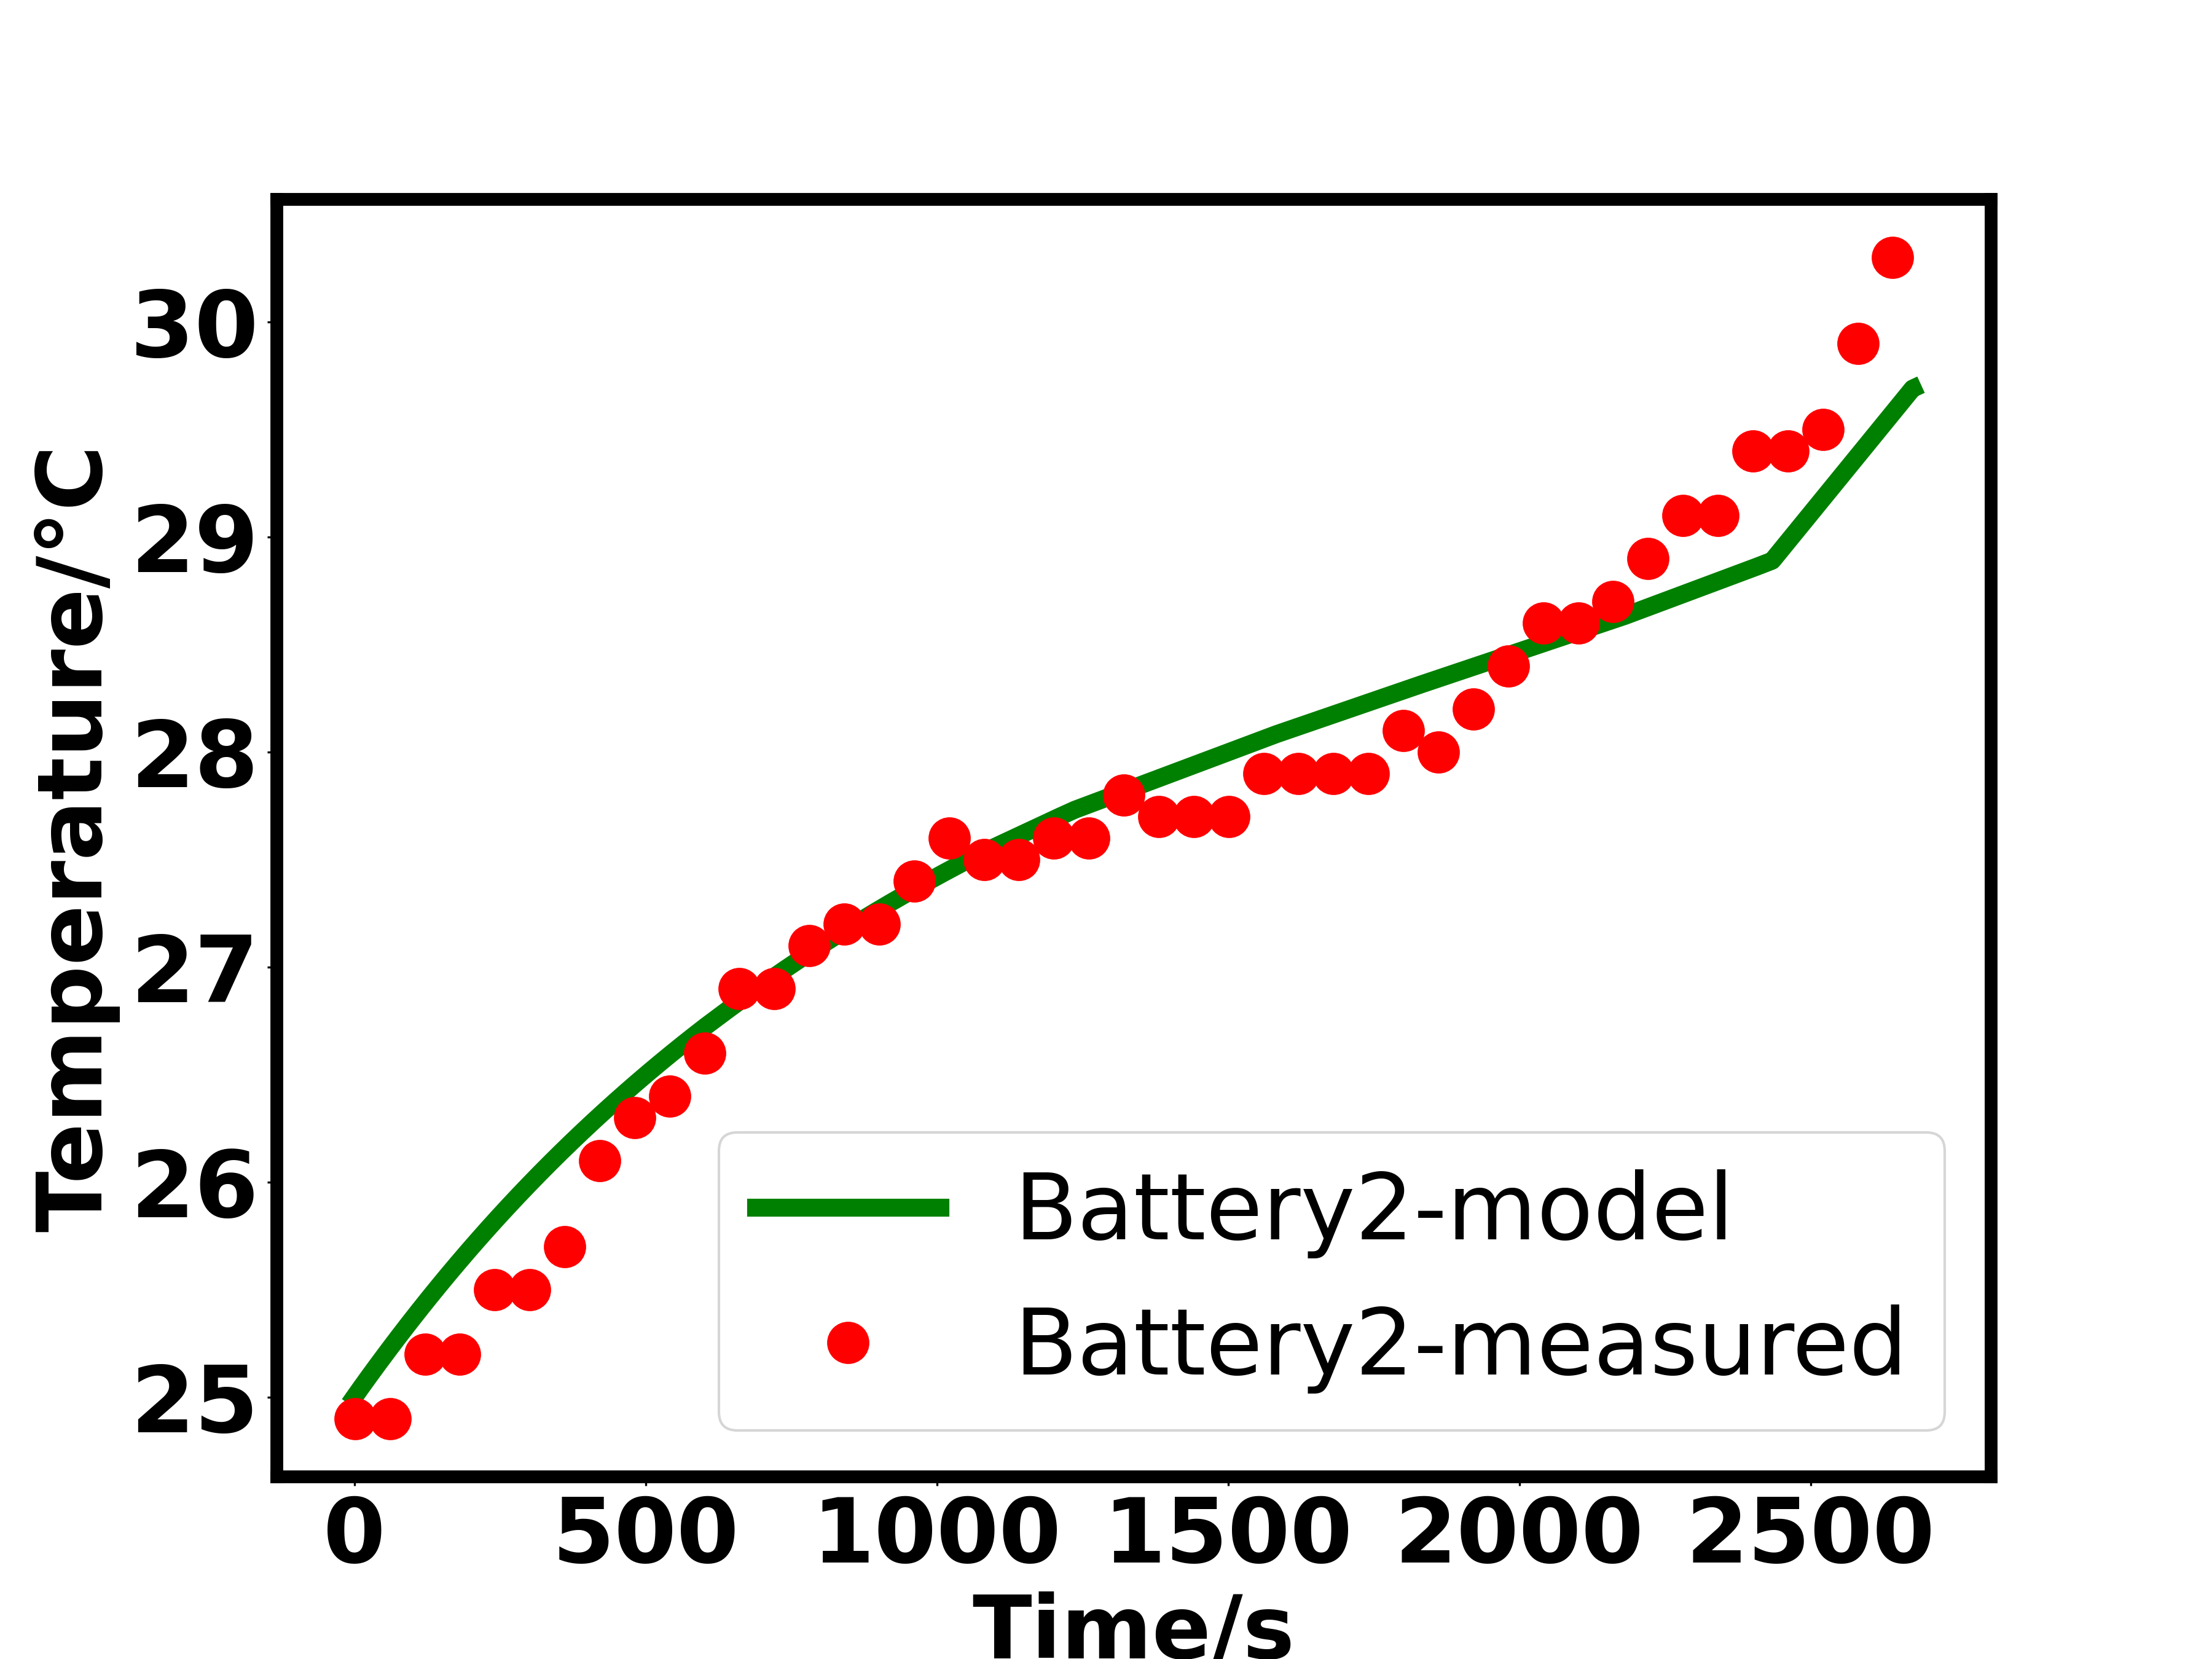
\includegraphics[width=\linewidth]{cell2_temperature_fit.png}
\end{minipage}%
}\par\smallskip
\subfloat[Cell 3 voltage]{%
\begin{minipage}[t]{0.48\columnwidth}
\centering
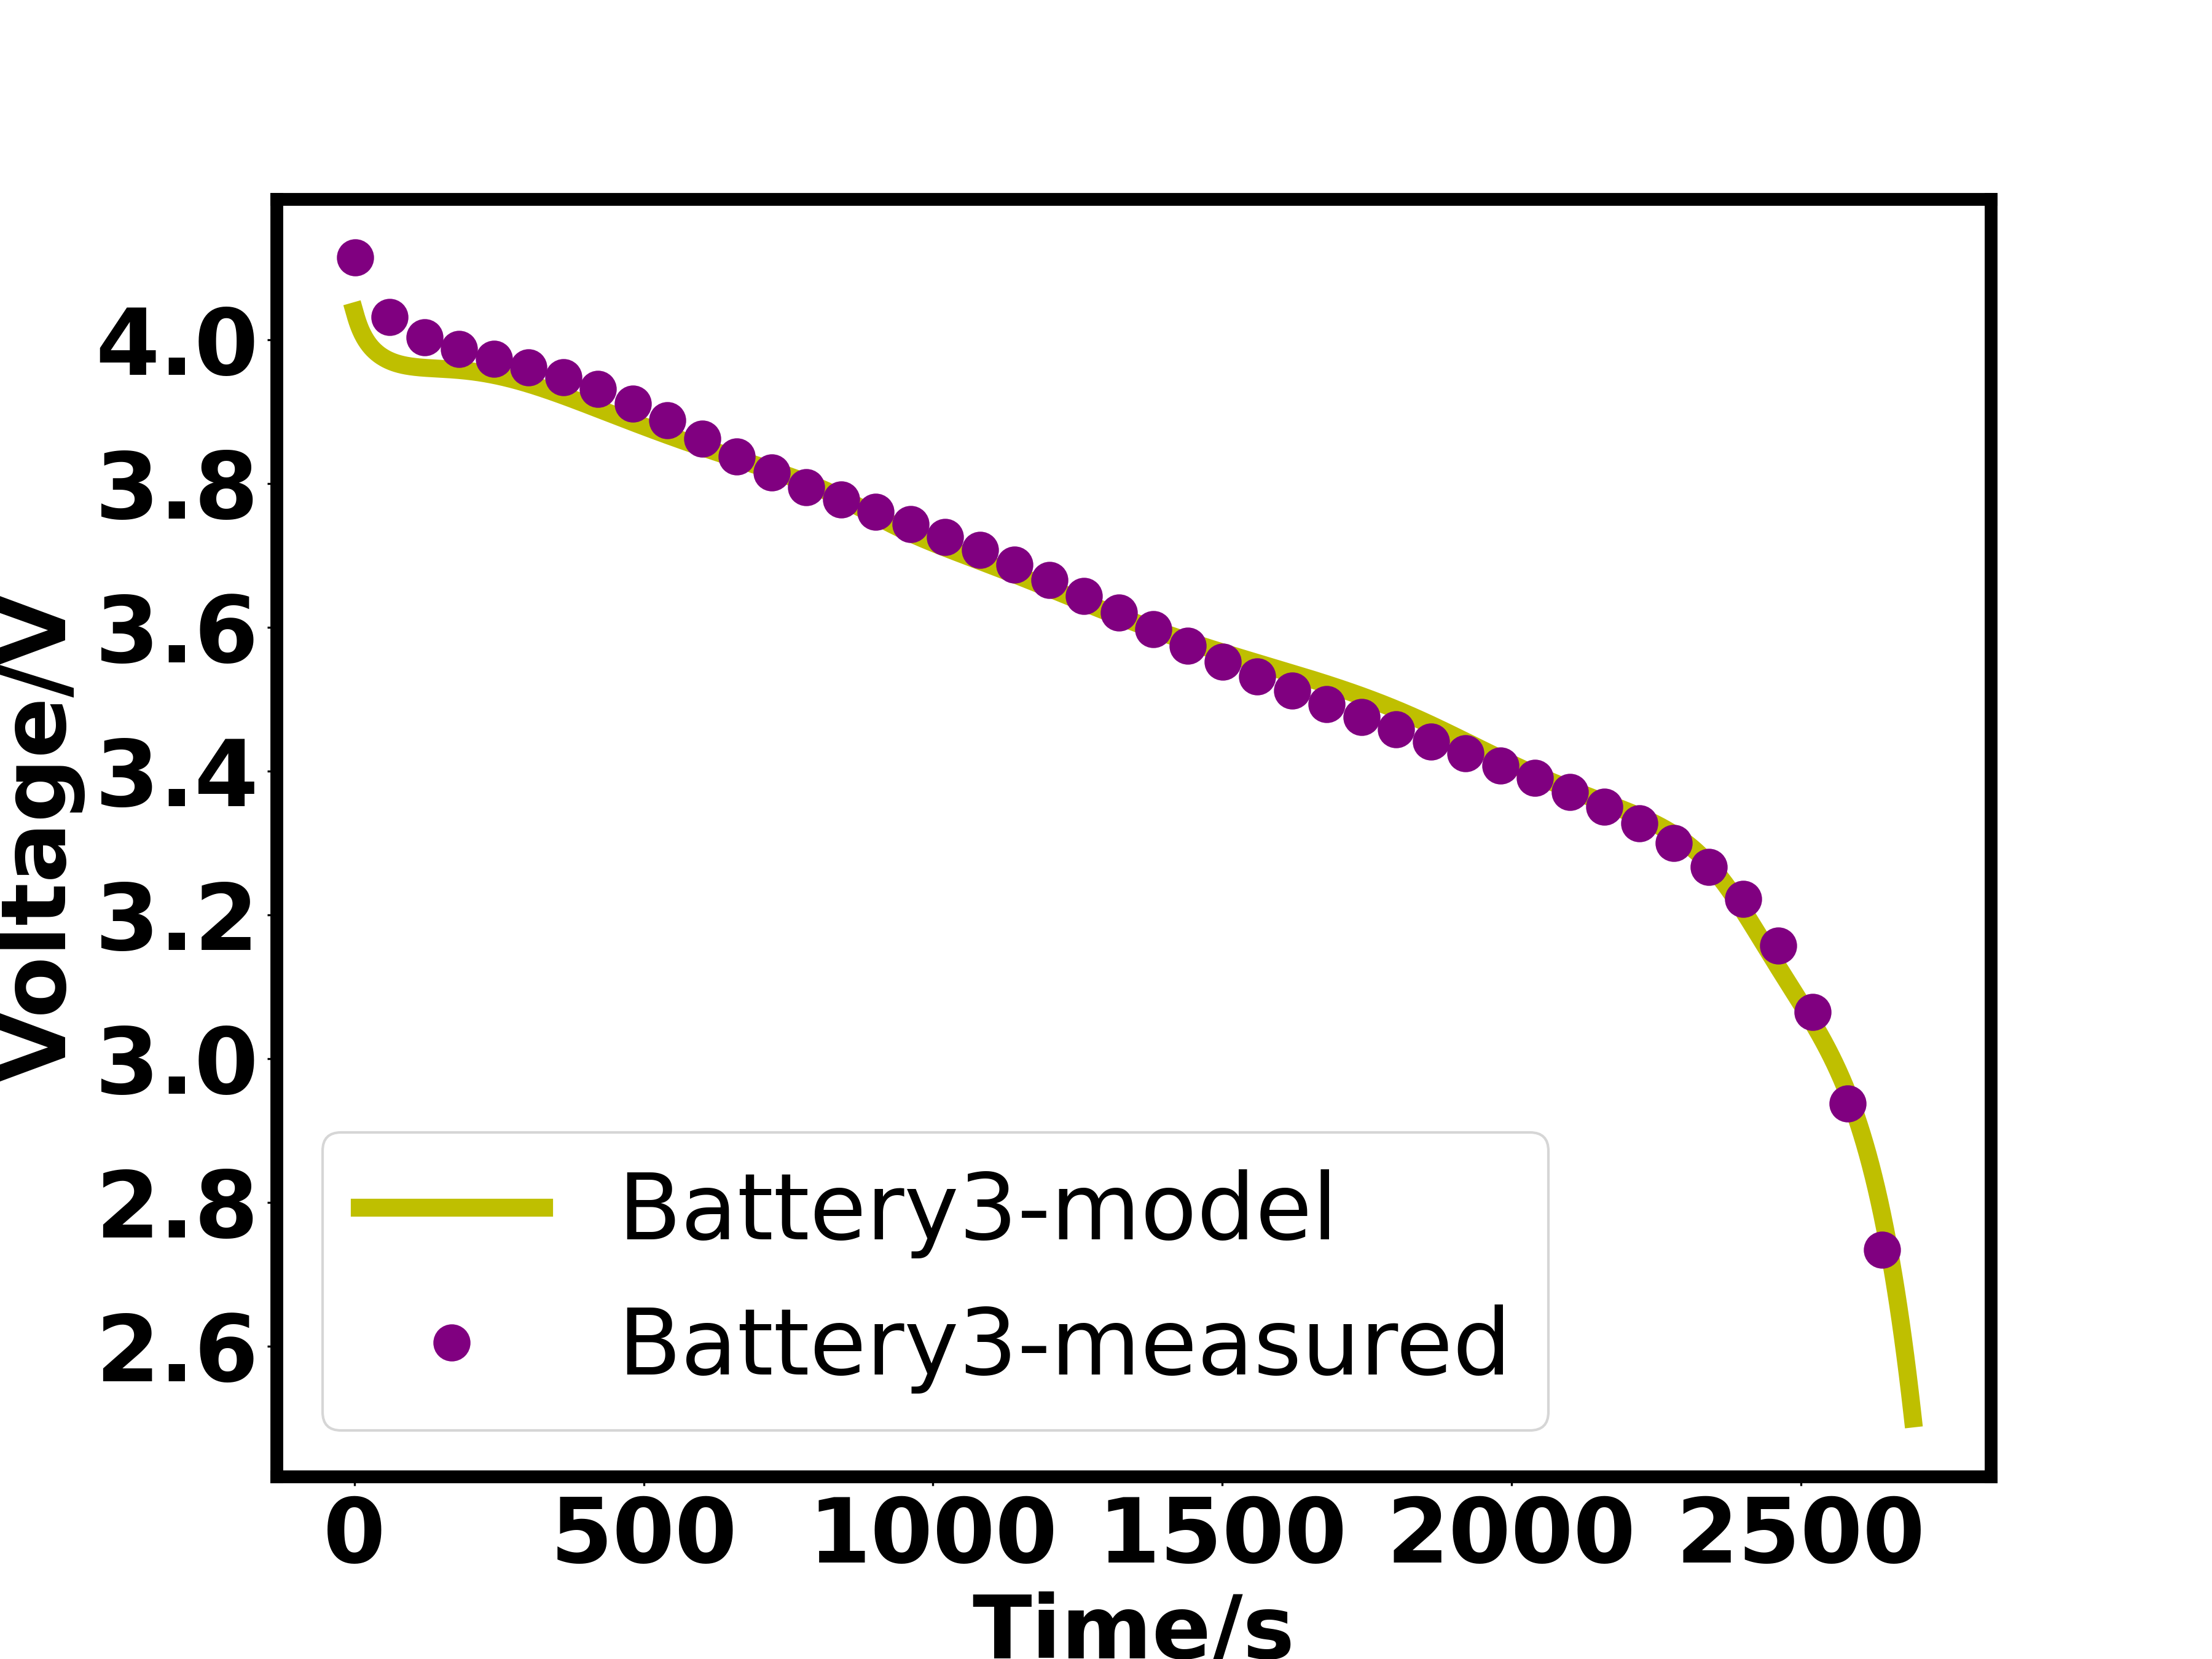
\includegraphics[width=\linewidth]{cell3_voltage_fit.png}
\end{minipage}%
}\hfill
\subfloat[Cell 3 temperature]{%
\begin{minipage}[t]{0.48\columnwidth}
\centering
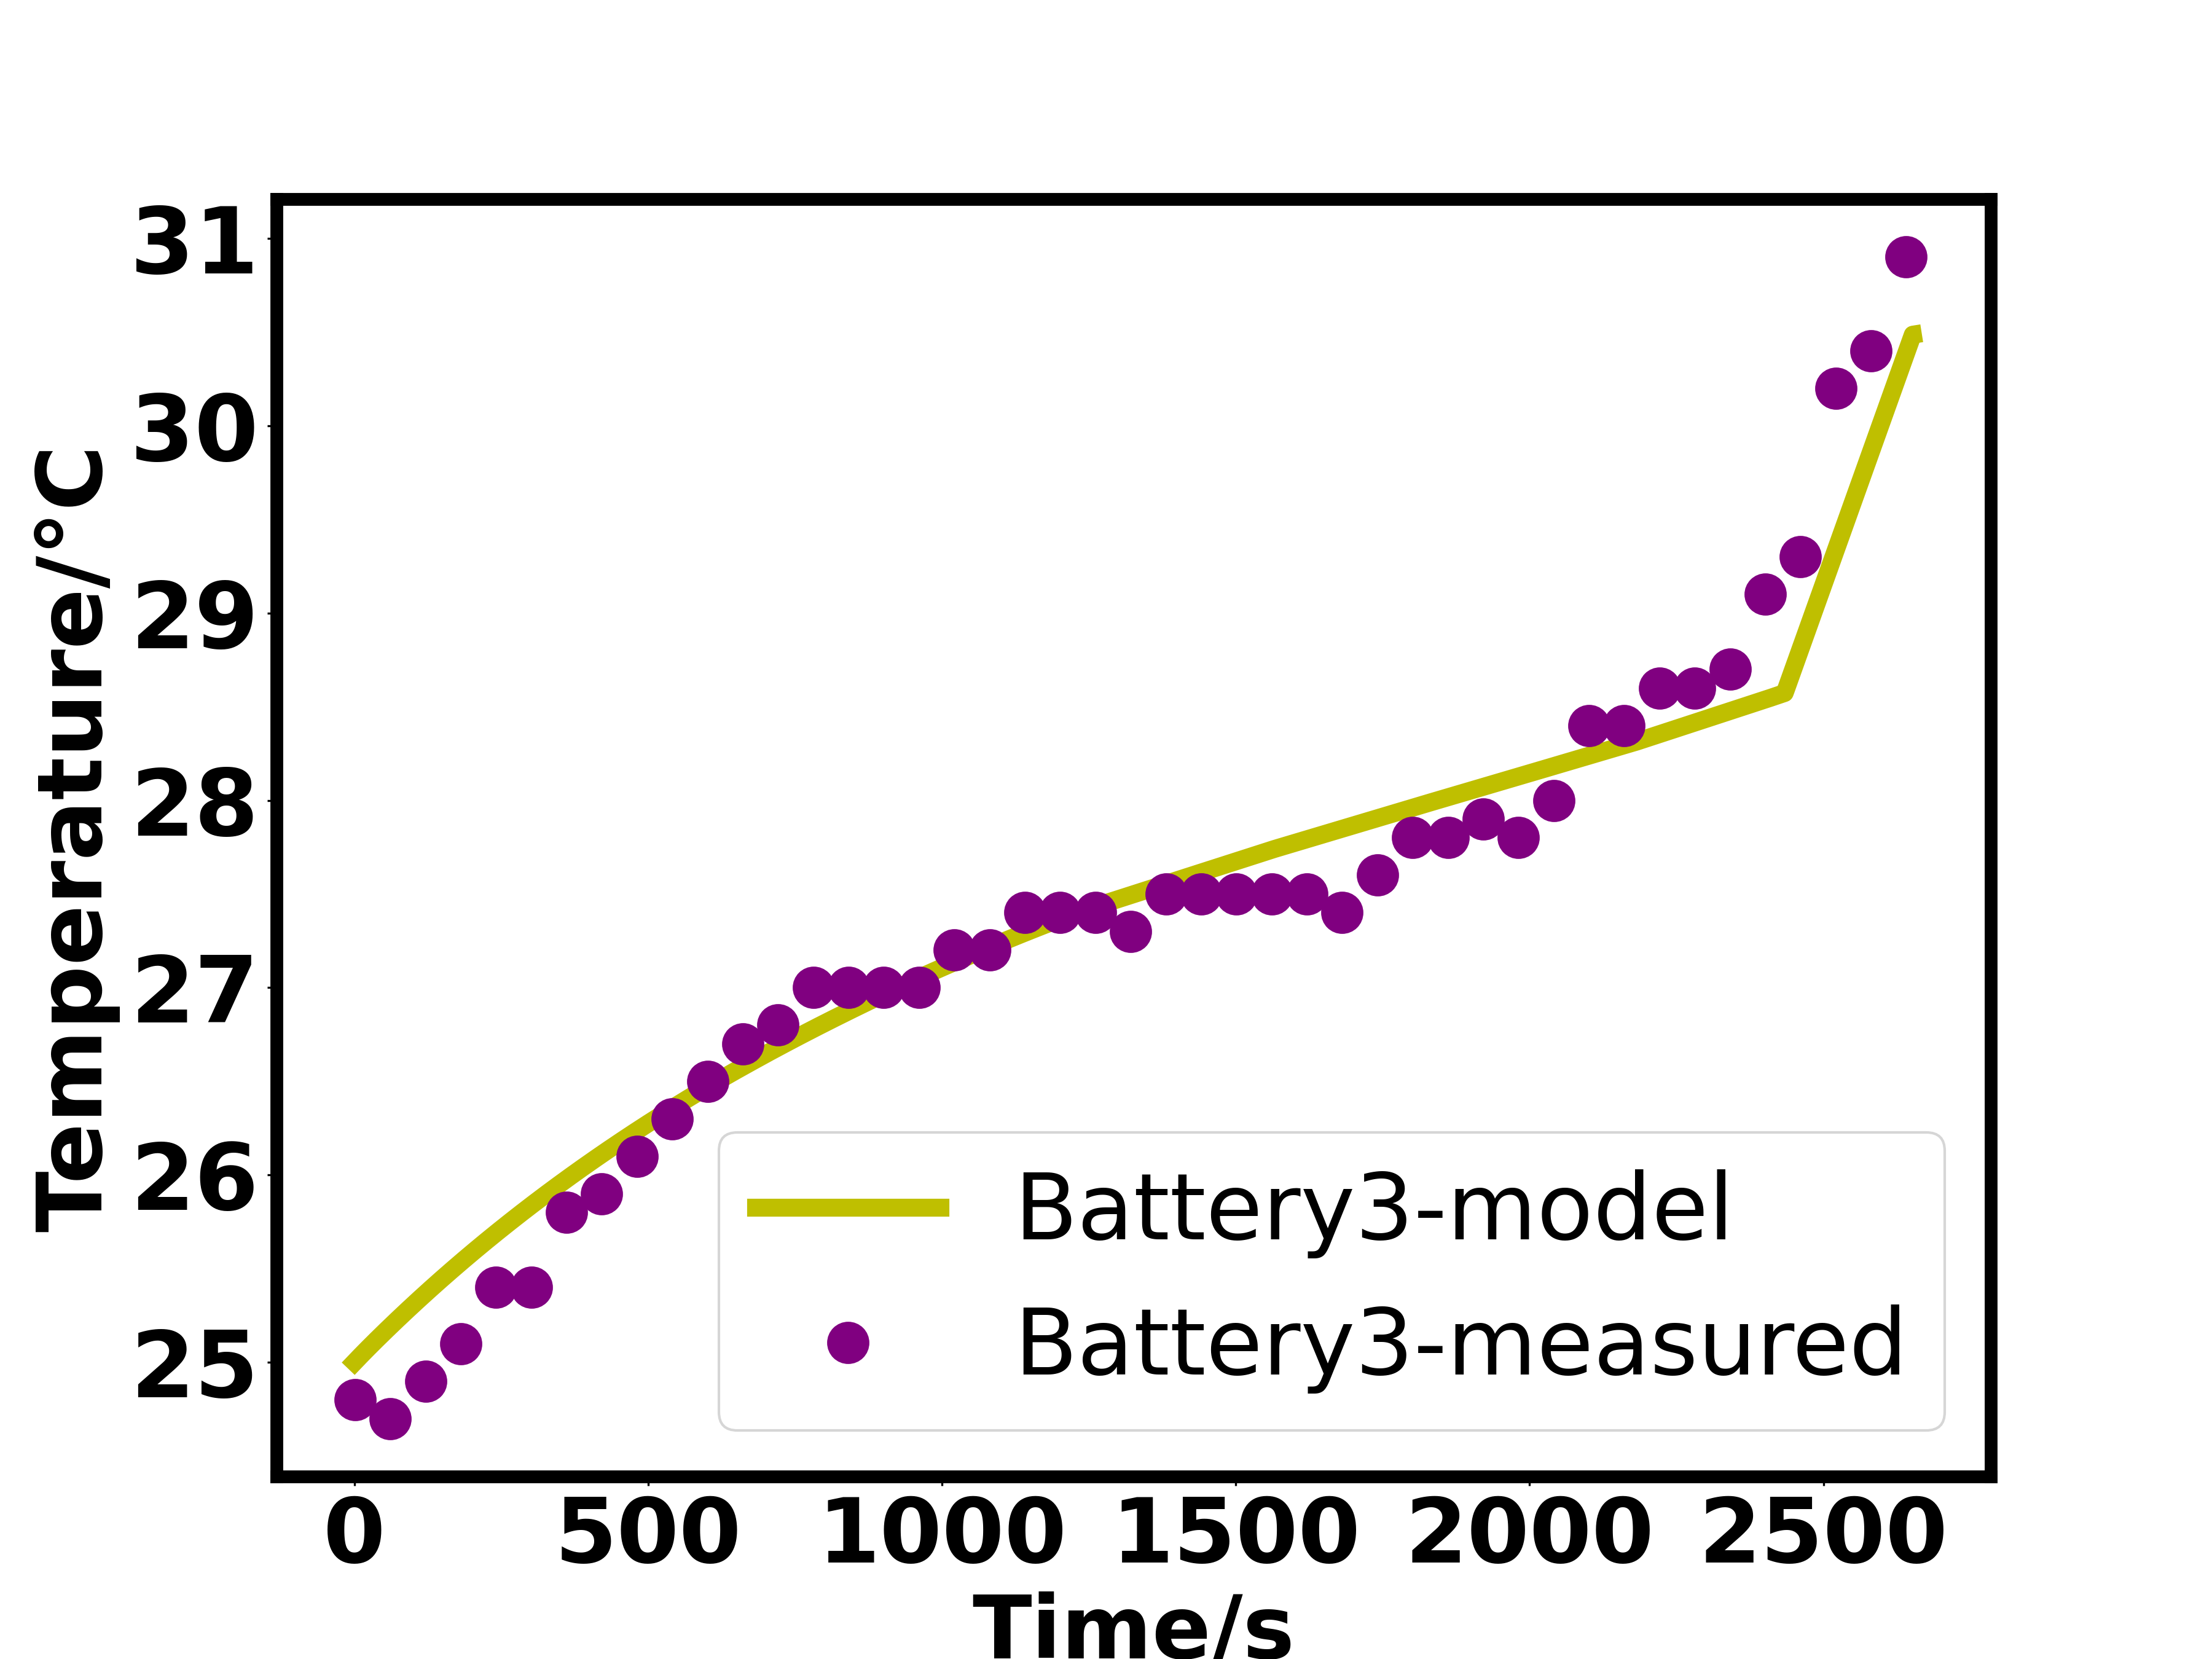
\includegraphics[width=\linewidth]{cell3_temperature_fit.png}
\end{minipage}%
}
\caption{Measured and SPMe-predicted voltage and temperature for the three cells.}
\label{fig:cell_validation}
\end{figure}

\begin{table}[!t]
\centering
\caption{RMSE values for the three identified cells}
\label{tab:cell_rmse}
\begin{tabular}{@{}lcc@{}}
\toprule
Cell & Voltage RMSE (V) & Temperature RMSE ($^\circ$C) \\
\midrule
Cell 1 & 0.026 & 0.068 \\
Cell 2 & 0.035 & 0.091 \\
Cell 3 & 0.029 & 0.093 \\
\bottomrule
\end{tabular}
\end{table}

\subsection{Performance Evaluation of MBA-RL}

The identified cell models were implemented in PyBaMM \cite{29} for the charging-control evaluations. Unless otherwise stated, the operating limits and training settings follow Tables~\ref{tab:experimental_settings} and \ref{tab:training_settings}. Two initial SOC vectors, $Set\;A=[10,20,30]^{\mathrm{T}}$ and $Set\;B=[30,50,70]^{\mathrm{T}}$ (in percent), are used as representative cases in Fig.~\ref{fig:overall_figure} and Table~\ref{tab:soc_vectors}. MBA-RL regulates the charging current of each cell directly, whereas DQL additionally controls a cell-to-cell energy-transfer topology and the CC-CV baseline activates the equalization topology during the CV phase.

\begin{figure}[!t]
\centering
\subfloat[MBA-RL, Set A]{%
\begin{minipage}[t]{0.48\columnwidth}
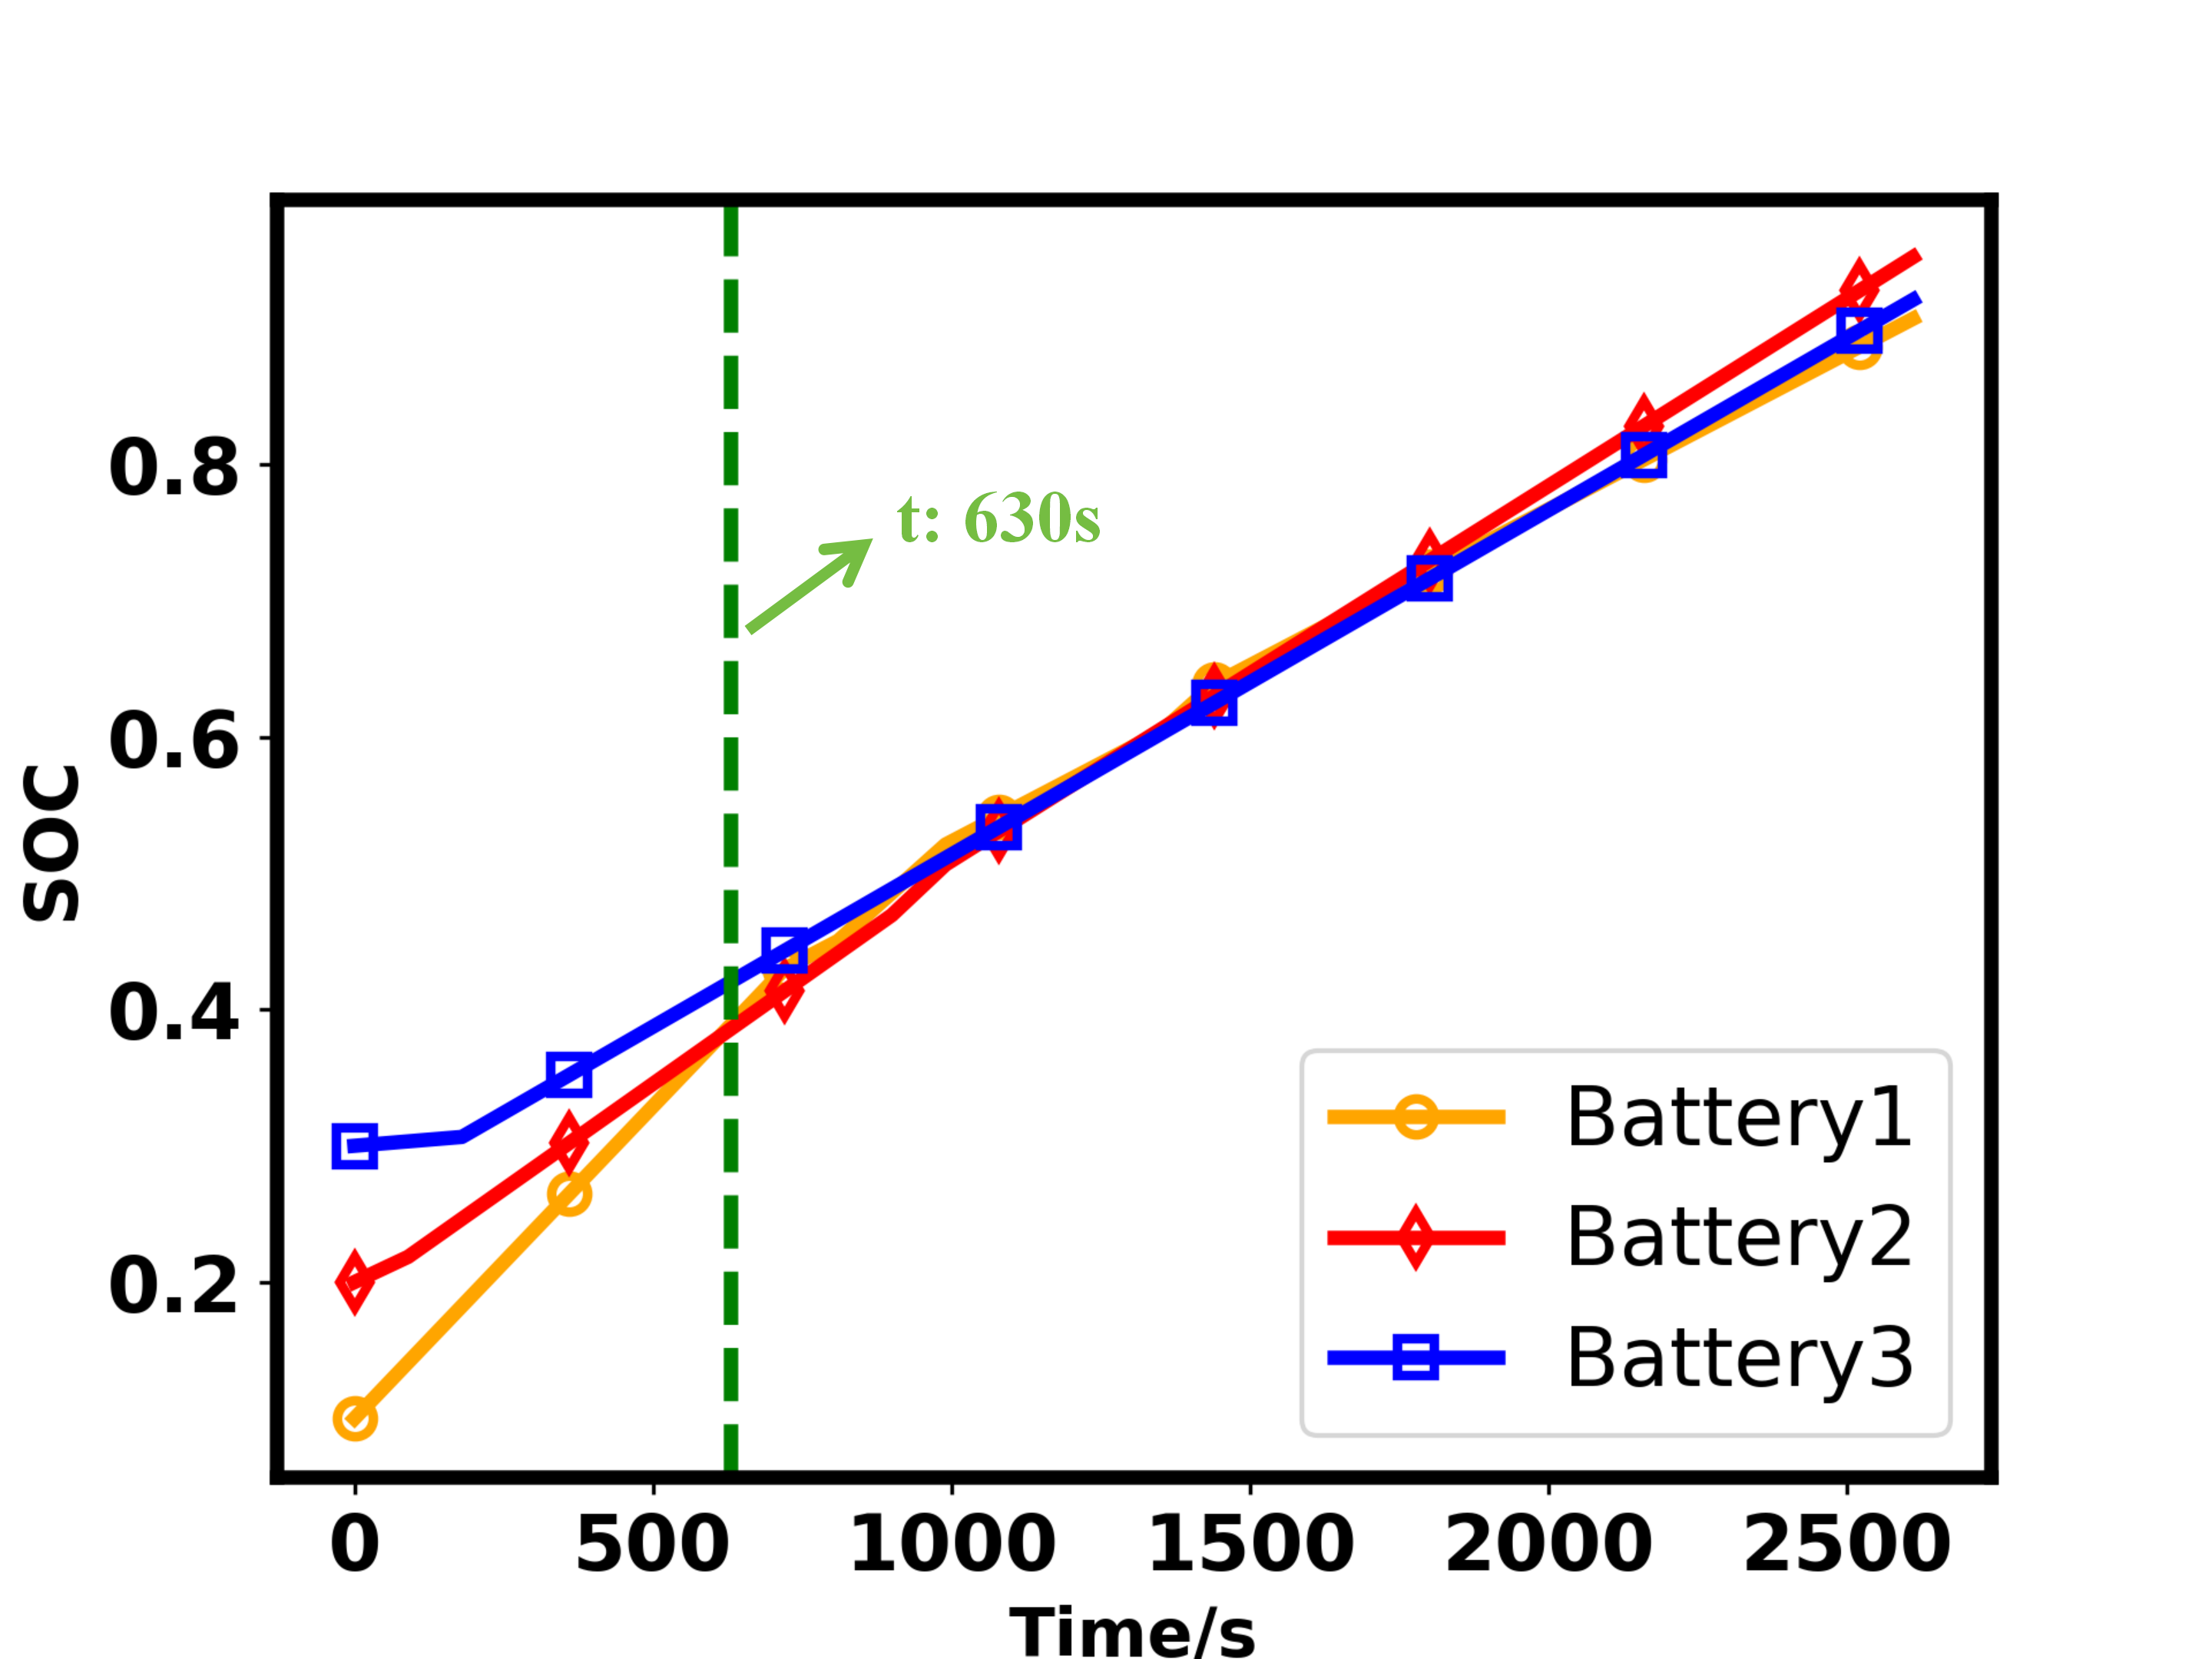
\includegraphics[width=\linewidth]{mba_rl_set_a.png}
\end{minipage}%
}\hfill
\subfloat[MBA-RL, Set B]{%
\begin{minipage}[t]{0.48\columnwidth}
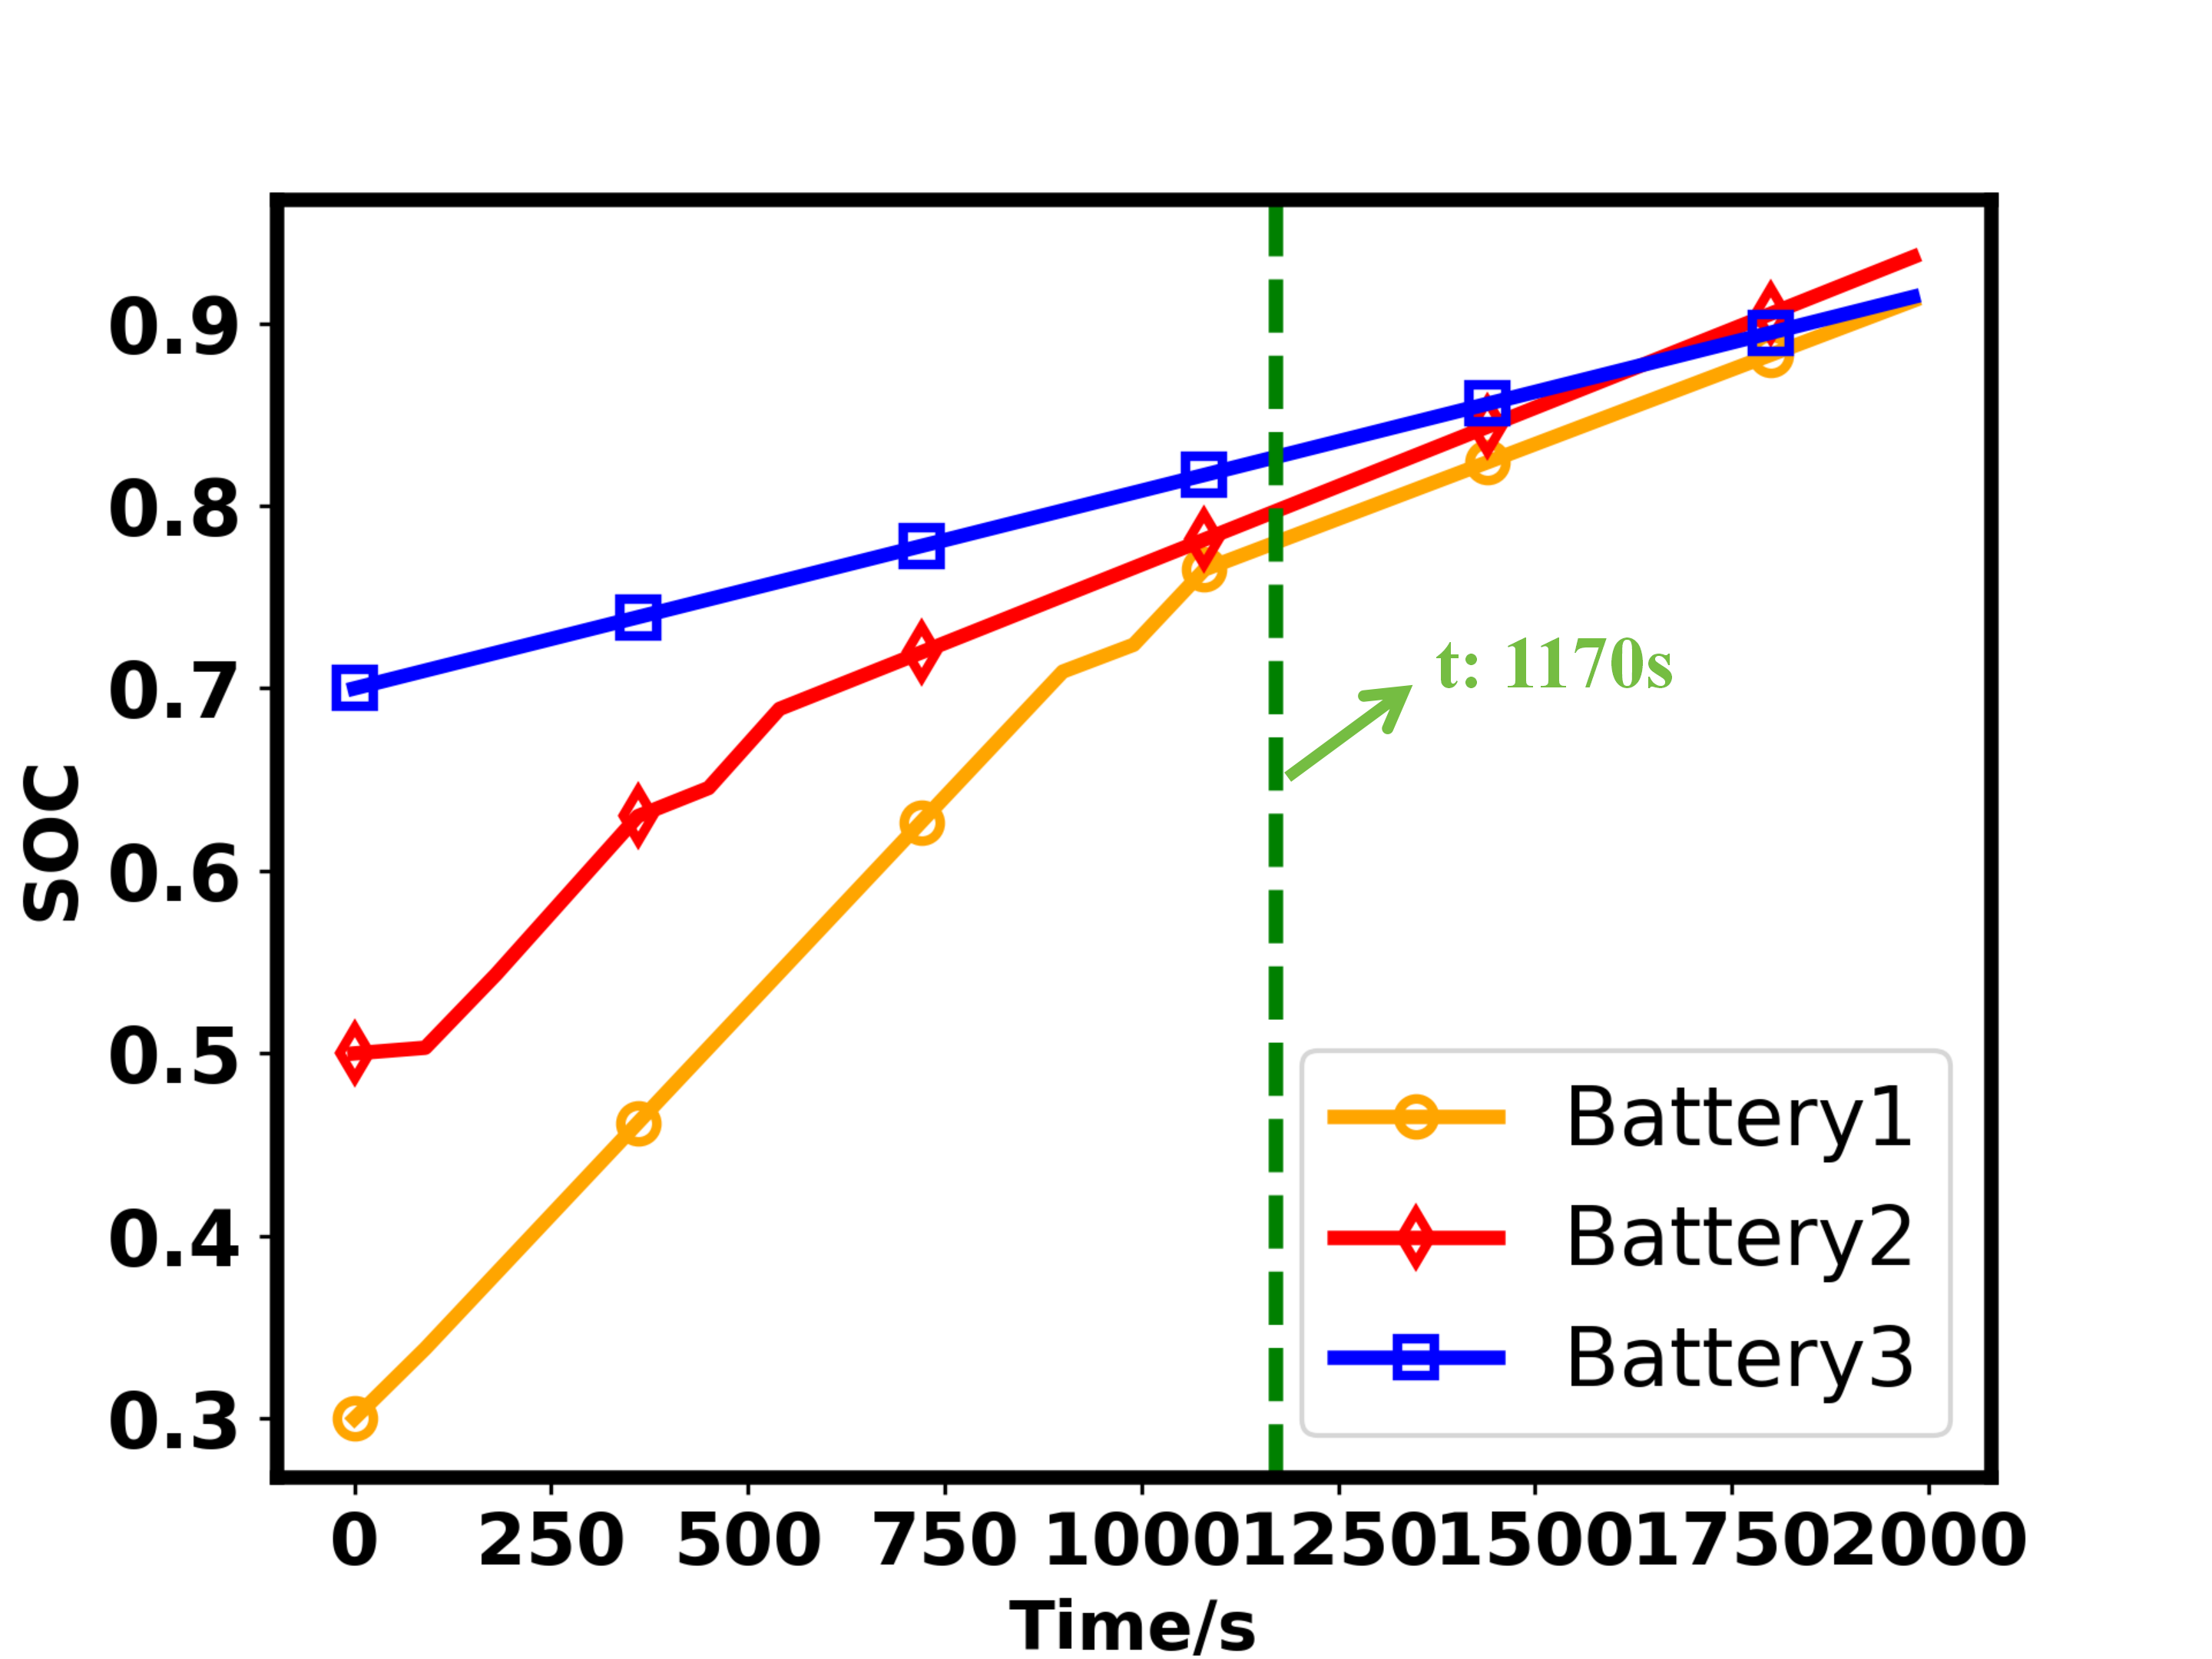
\includegraphics[width=\linewidth]{mba_rl_set_b.png}
\end{minipage}%
}\par\smallskip
\subfloat[DQL, Set A]{%
\begin{minipage}[t]{0.48\columnwidth}
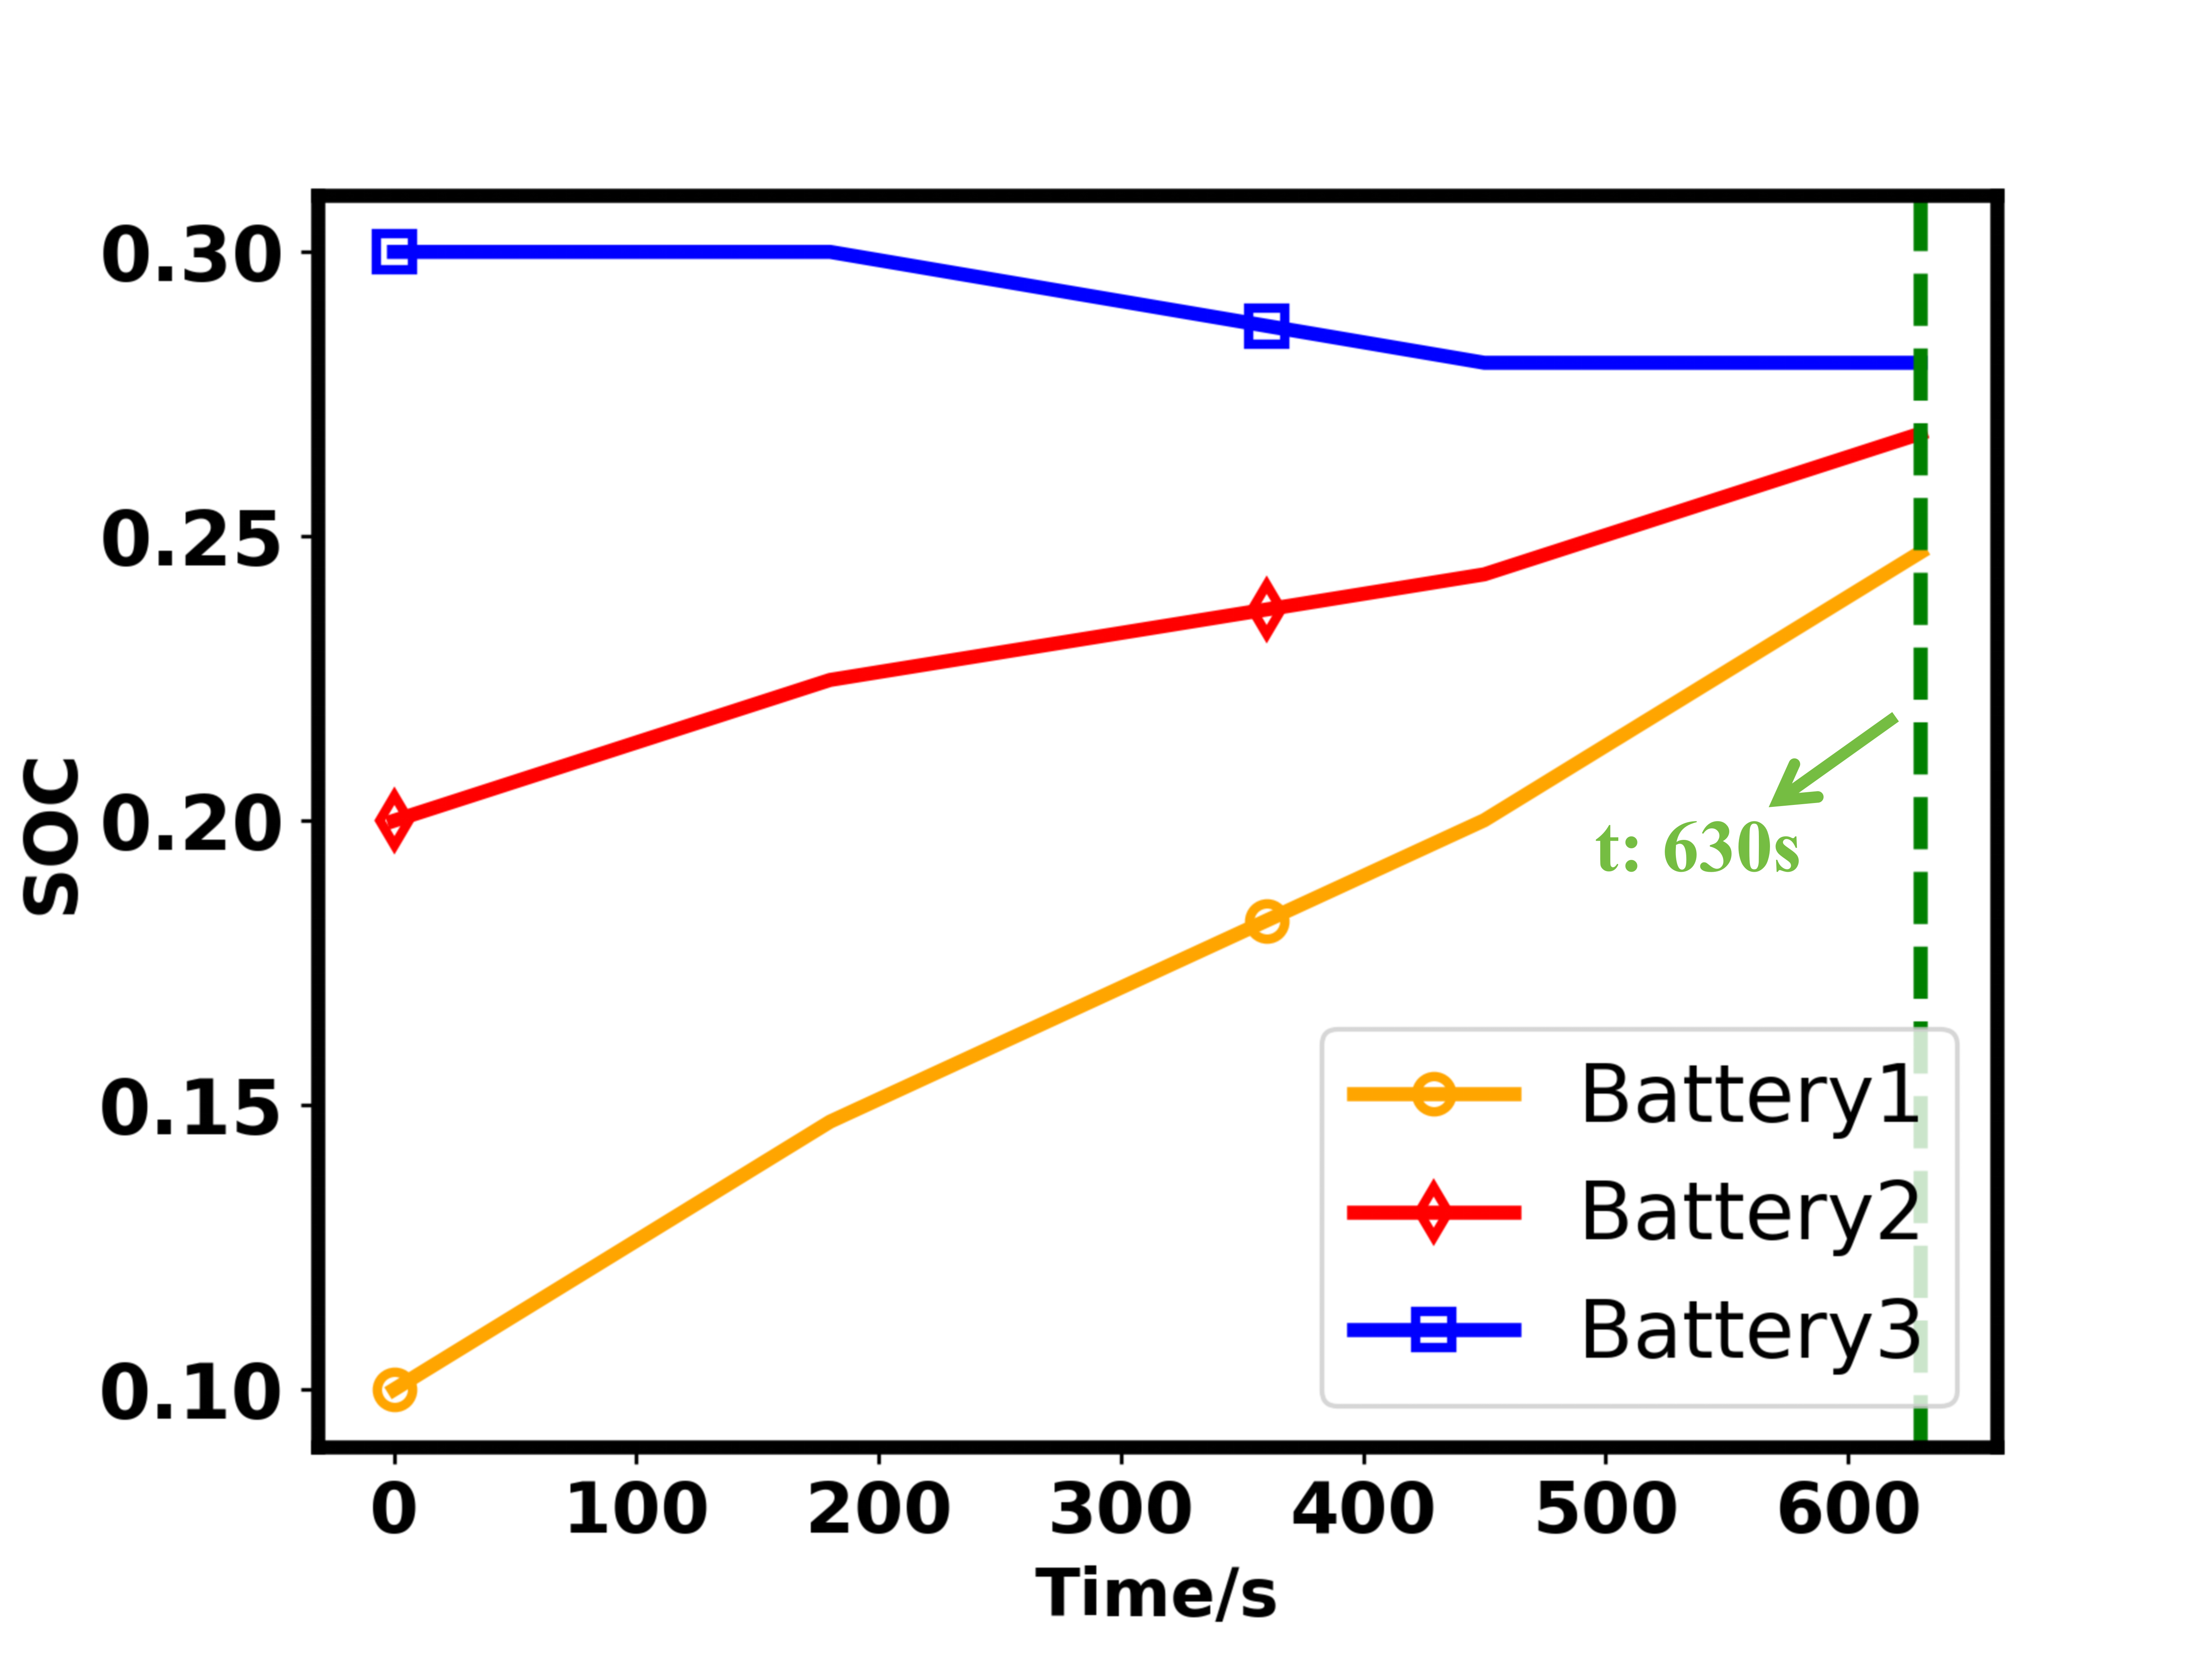
\includegraphics[width=\linewidth]{dql_set_a.png}
\end{minipage}%
}\hfill
\subfloat[DQL, Set B]{%
\begin{minipage}[t]{0.48\columnwidth}
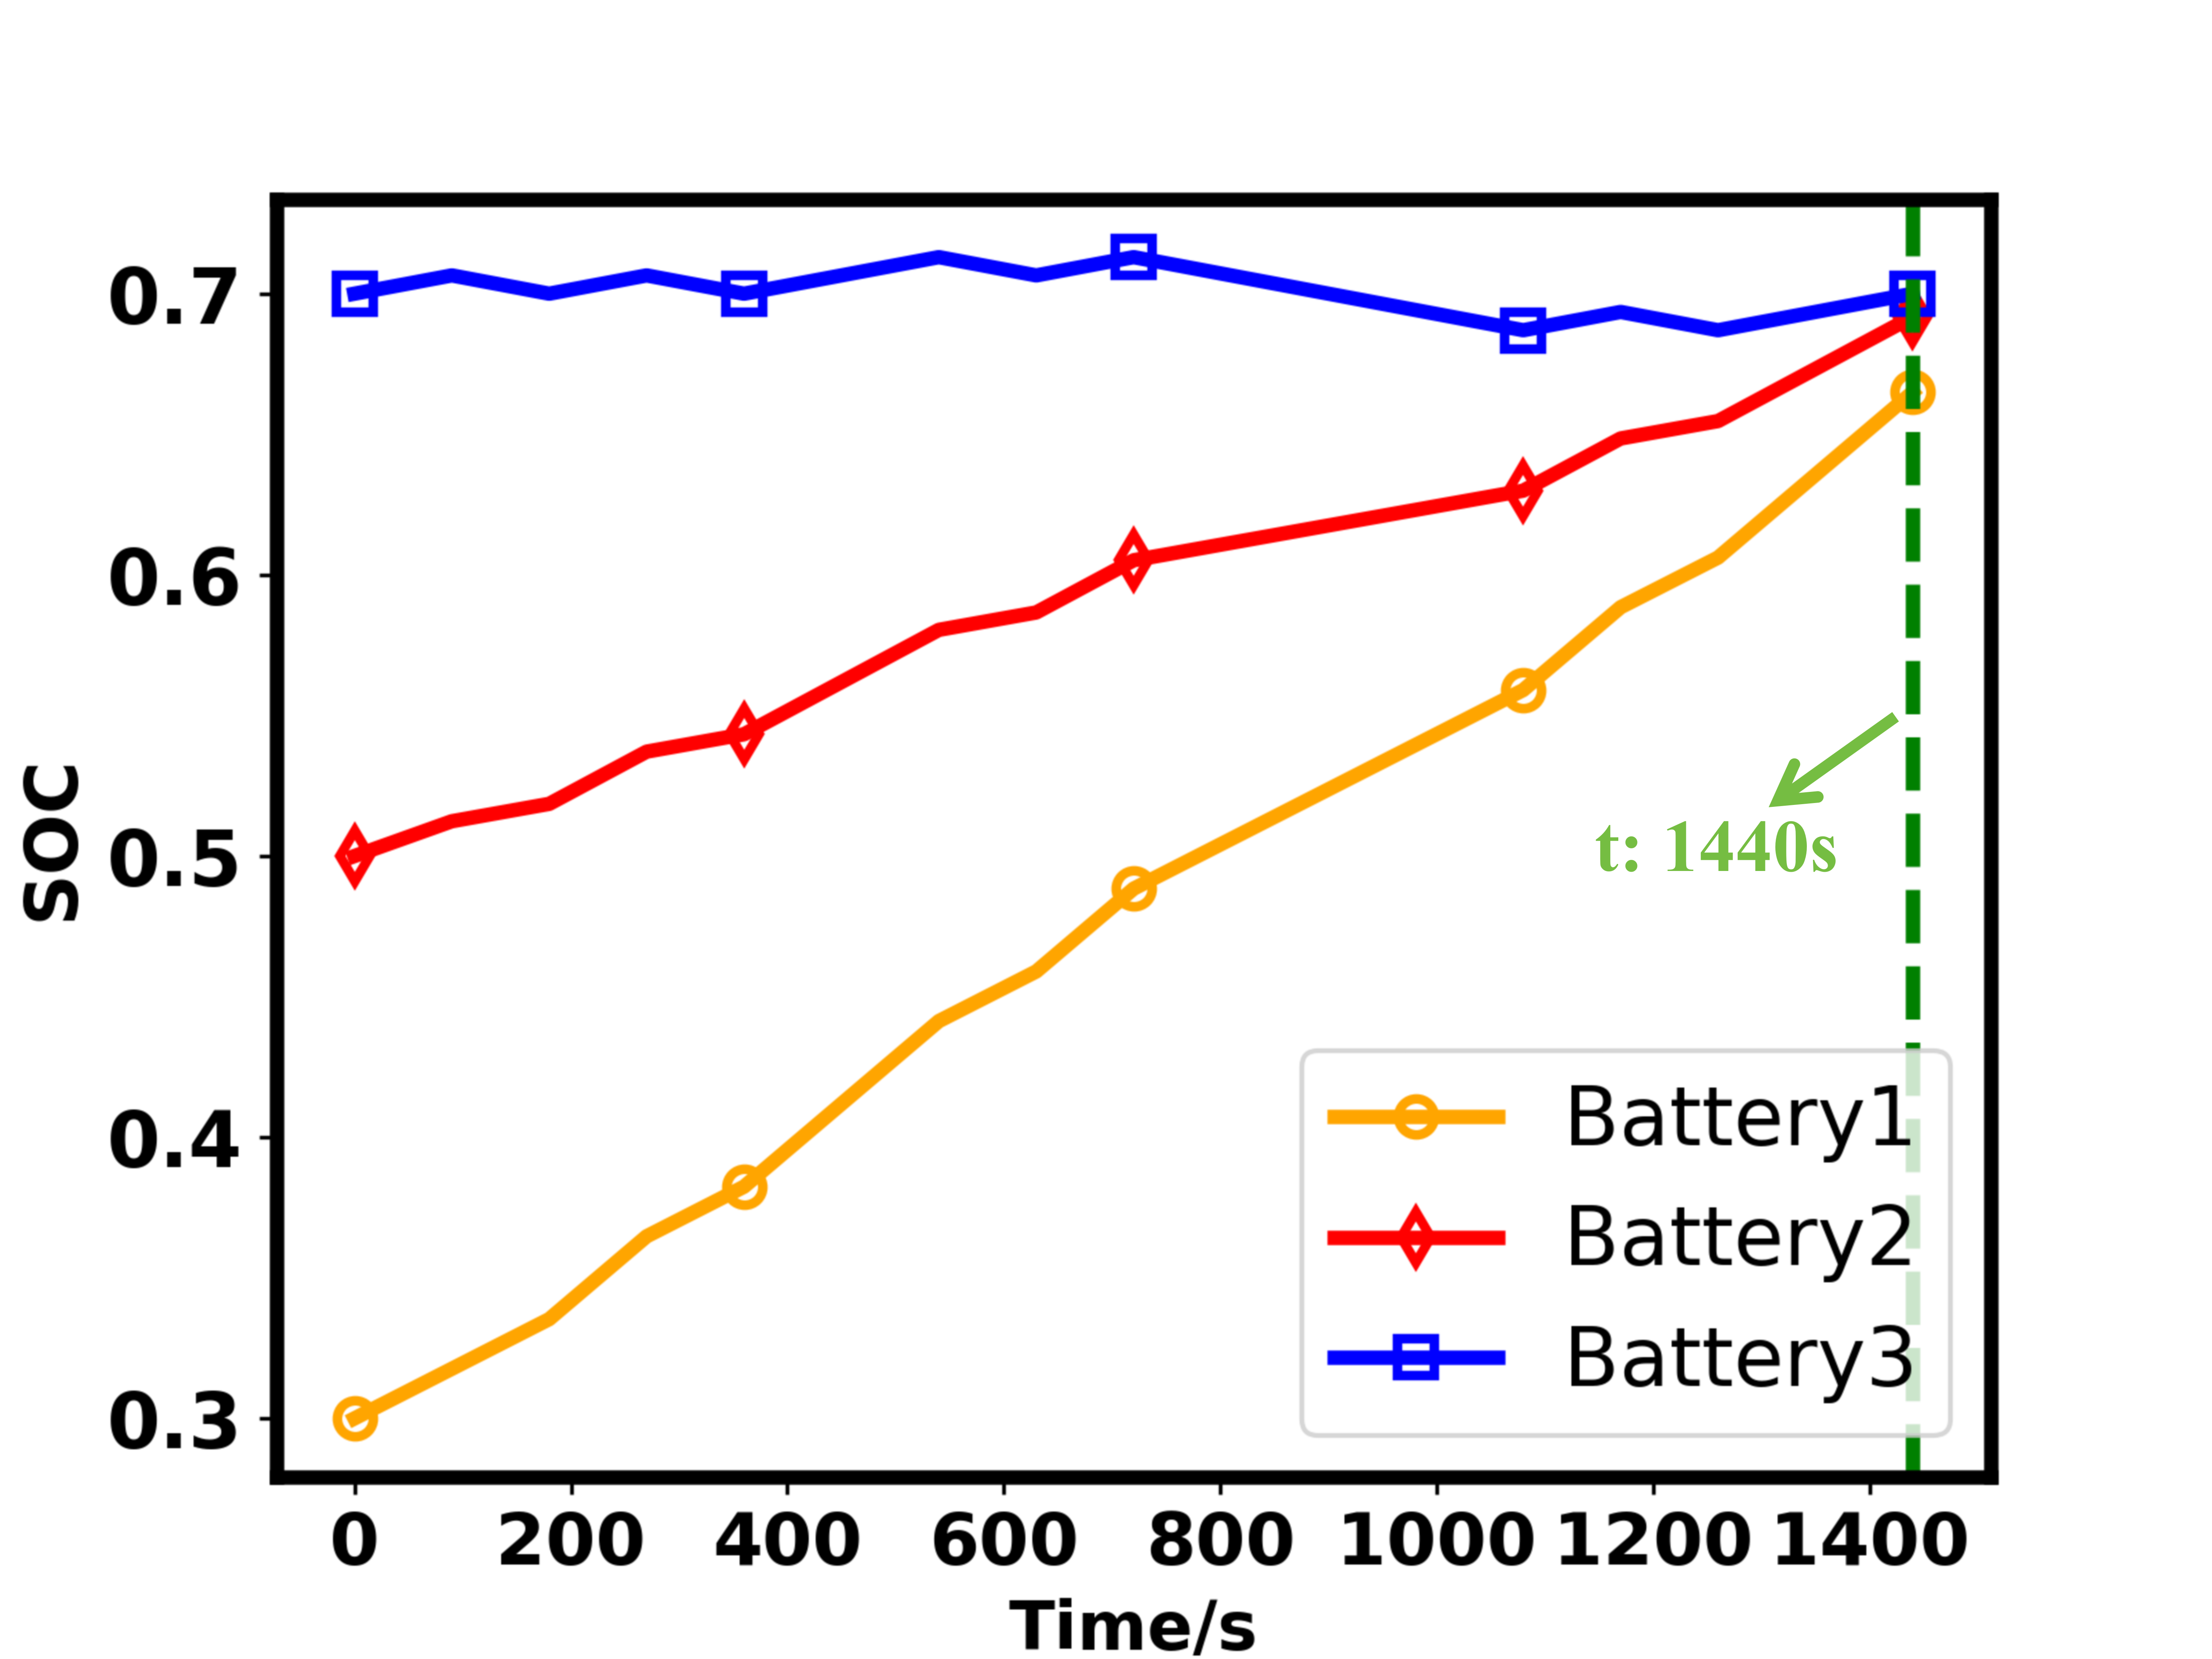
\includegraphics[width=\linewidth]{dql_set_b.png}
\end{minipage}%
}\par\smallskip
\subfloat[CC-CV, Set A]{%
\begin{minipage}[t]{0.48\columnwidth}
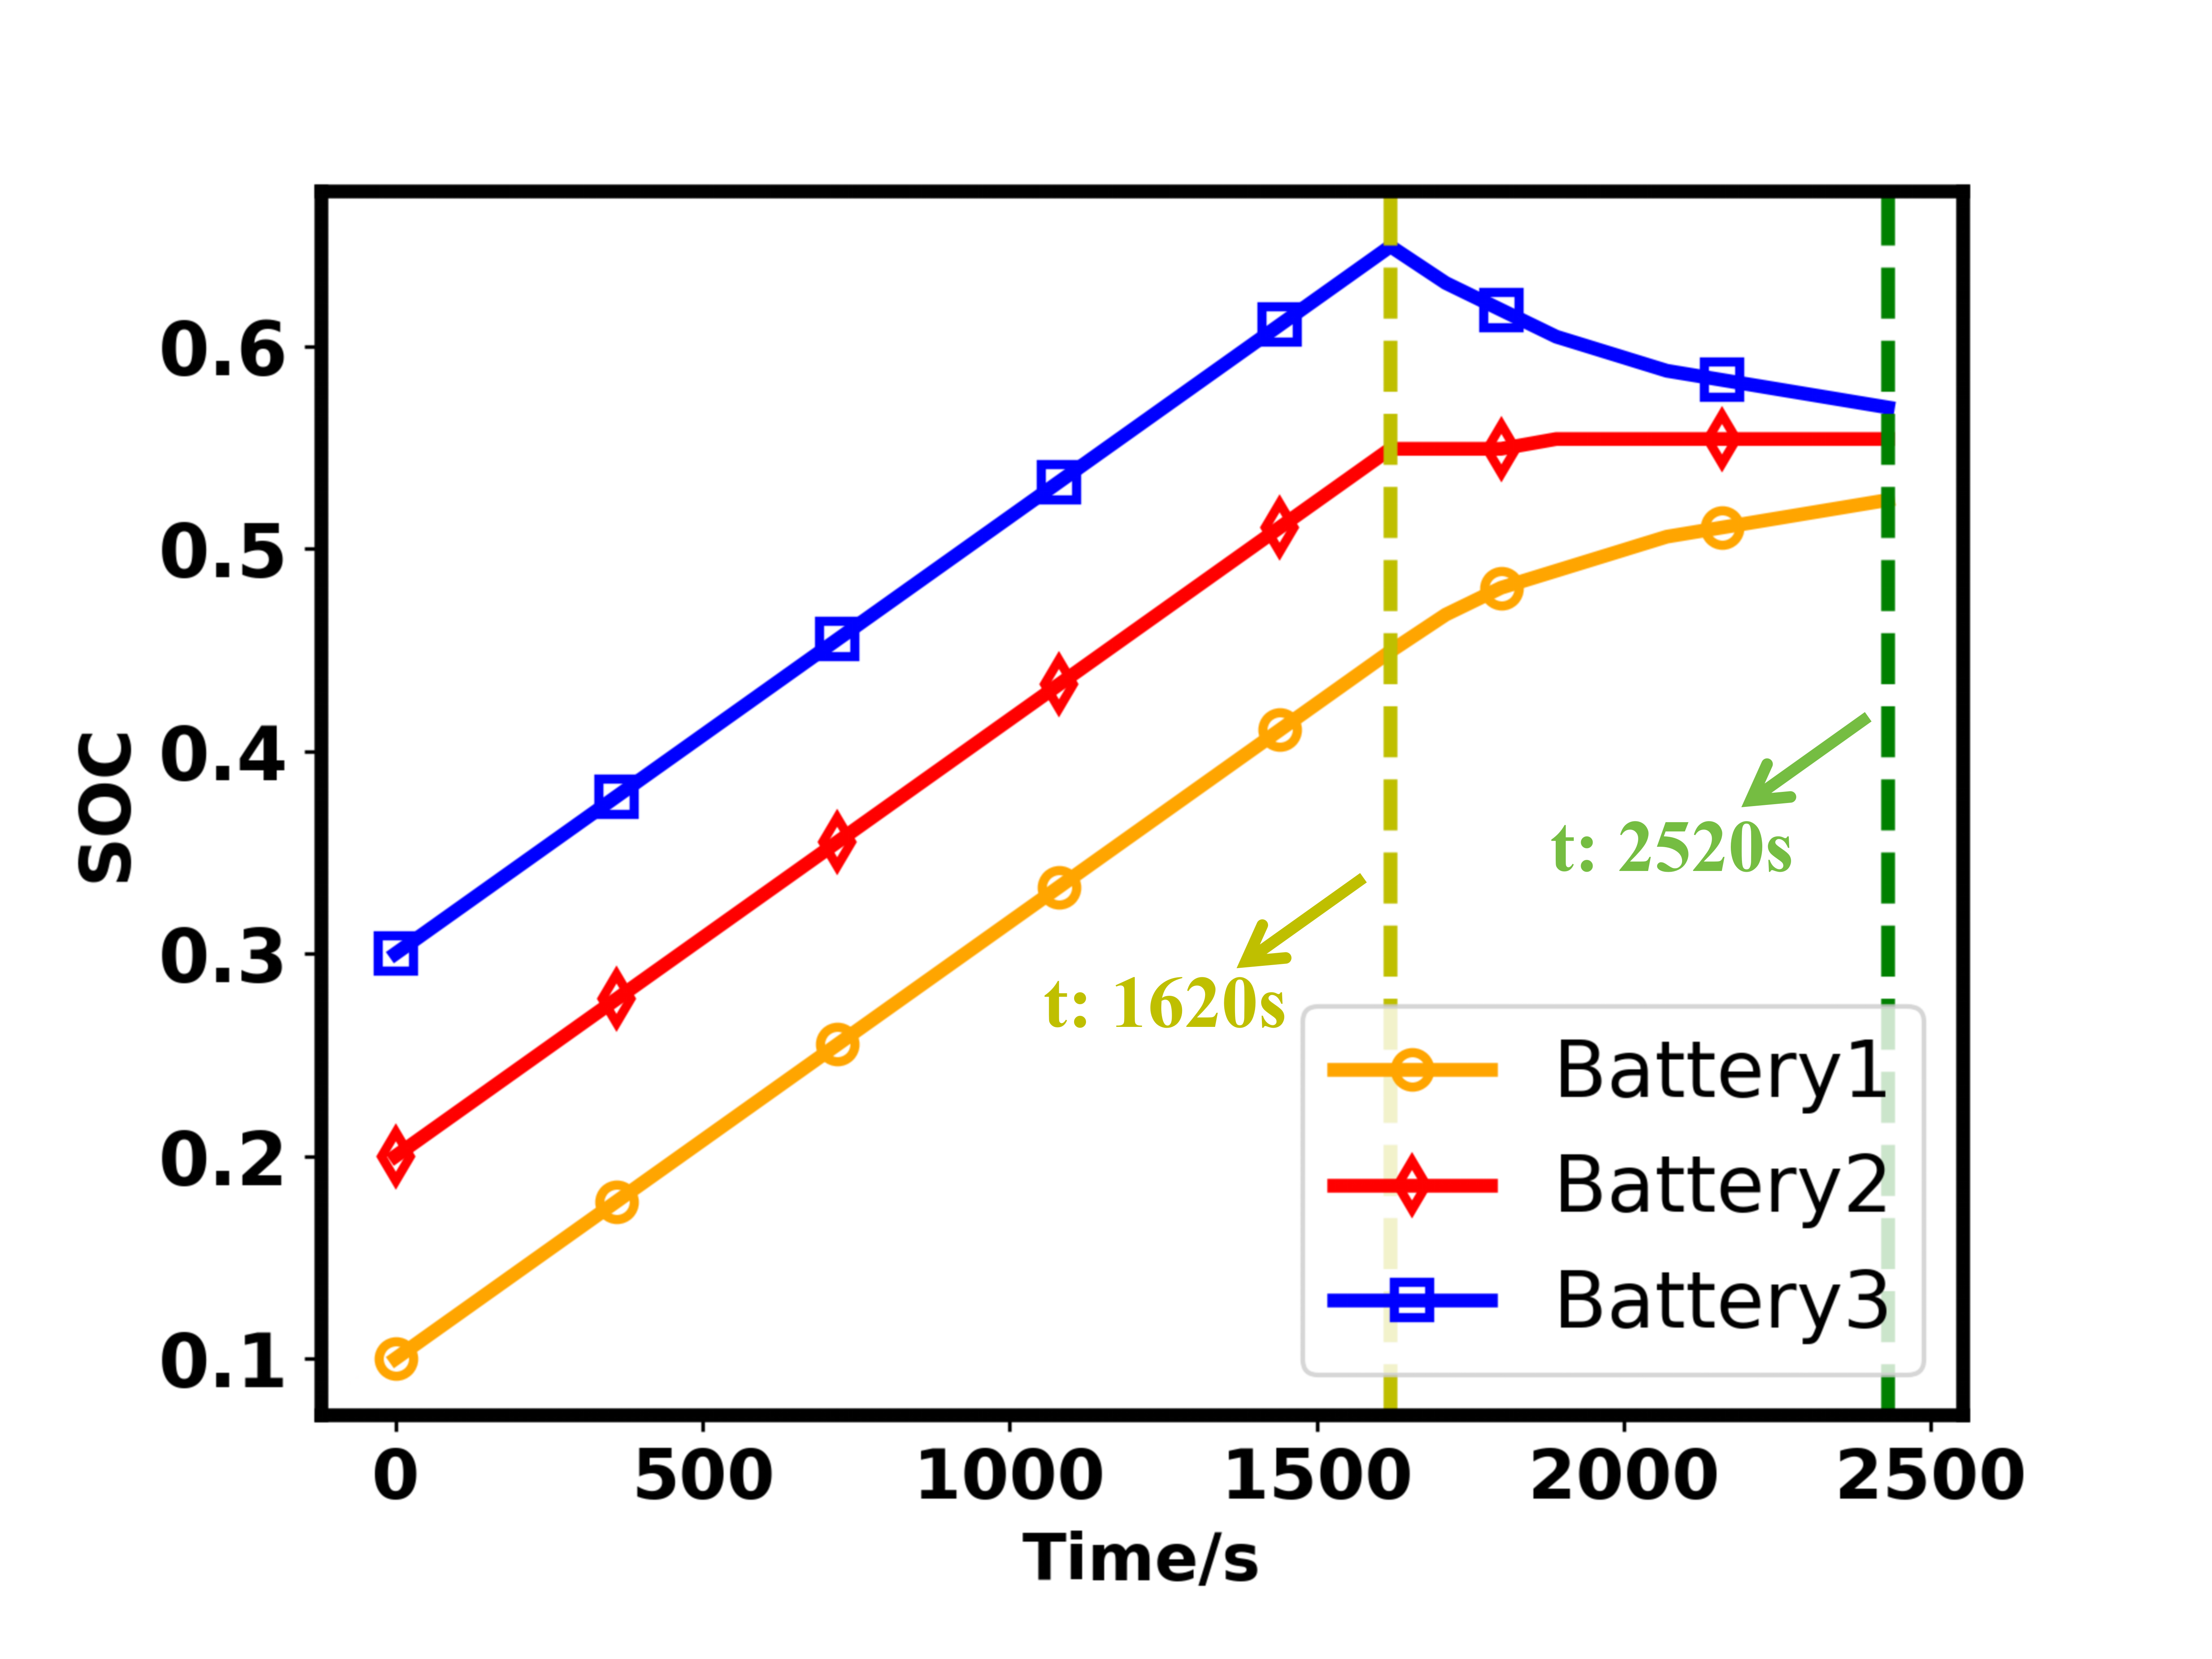
\includegraphics[width=\linewidth]{cc_cv_set_a.png}
\end{minipage}%
}\hfill
\subfloat[CC-CV, Set B]{%
\begin{minipage}[t]{0.48\columnwidth}
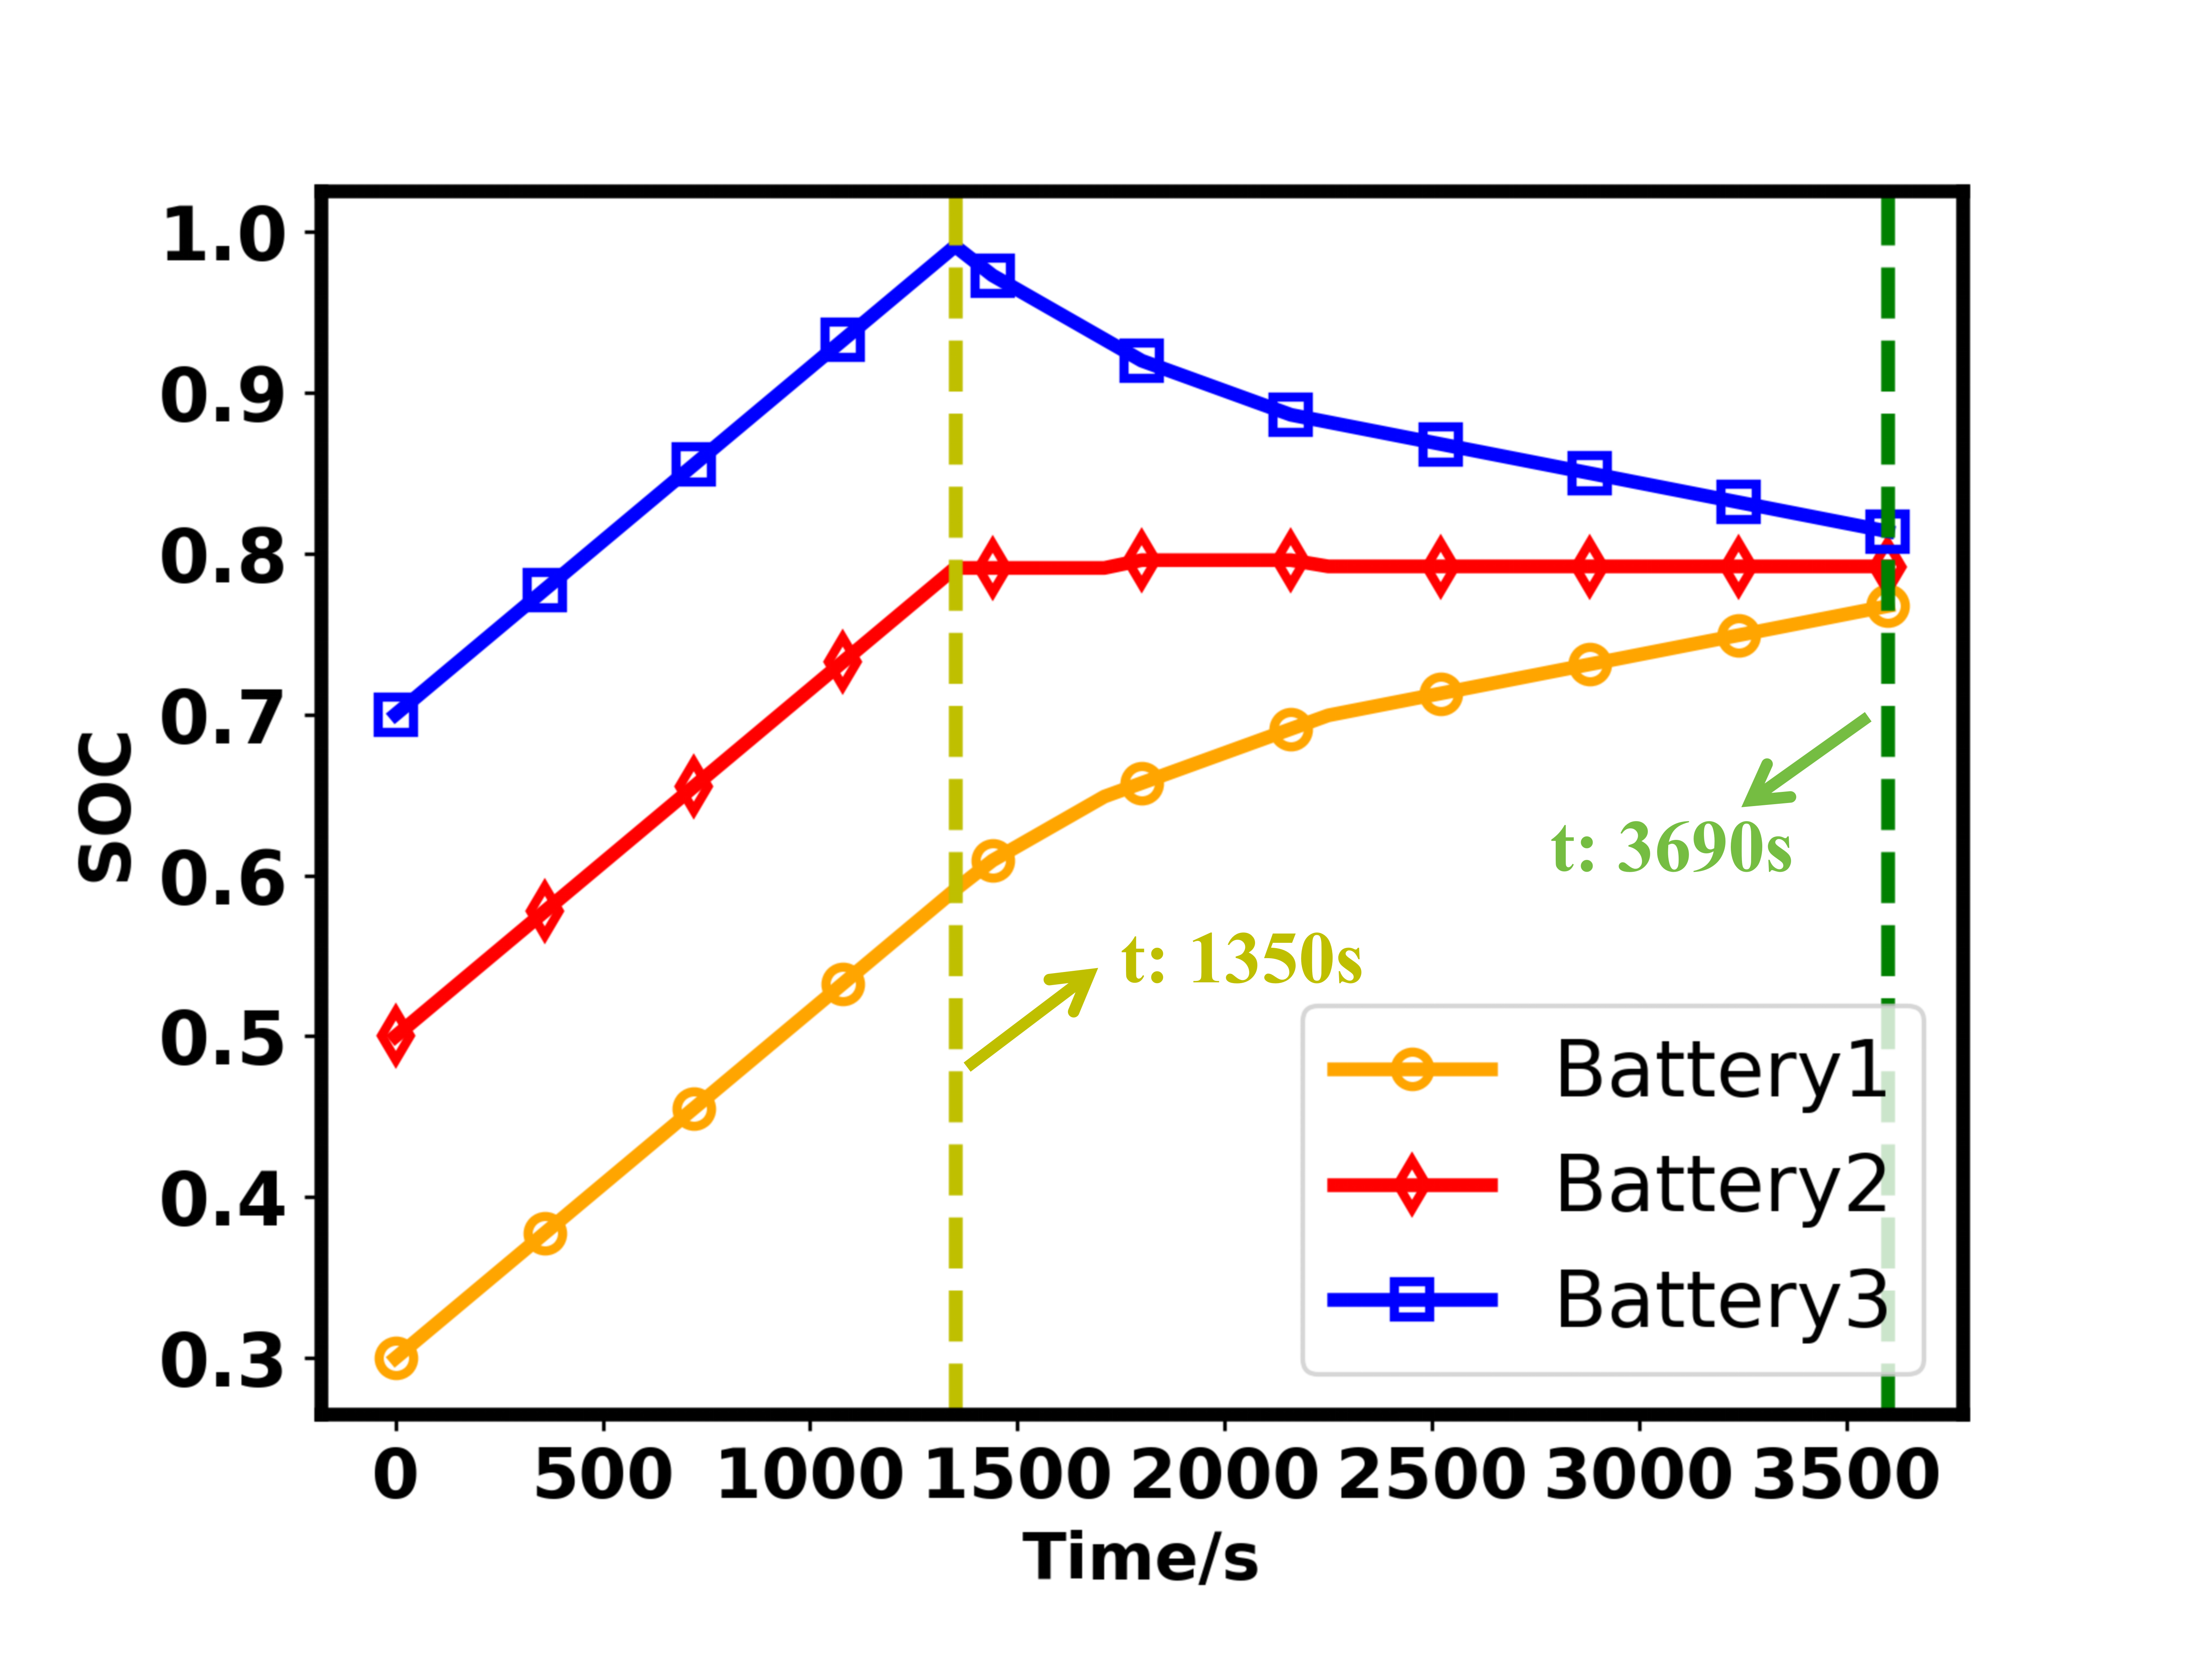
\includegraphics[width=\linewidth]{cc_cv_set_b.png}
\end{minipage}%
}
\caption{Charging trajectories for MBA-RL, DQL, and CC-CV. The green dashed line indicates the first time at which $\sigma\leq\beta$; the yellow dashed line marks the end of the CC phase.}
\label{fig:overall_figure}
\end{figure}

\begin{table}[!t]
\centering
\caption{Initial and terminal SOC vectors for the representative trajectories in Fig.~\ref{fig:overall_figure}}
\label{tab:soc_vectors}
\scriptsize
\setlength{\tabcolsep}{2pt}
\begin{tabular}{@{}lcc@{}}
\toprule
Method & Initial SOC (\%) & Terminal SOC (\%) \\
\midrule
MBA-RL & $[10,20,30]^{\mathrm T}$ & $[91.66,94.18,92.15]^{\mathrm T}$ \\
 & $[30,50,70]^{\mathrm T}$ & $[91.23,93.62,91.41]^{\mathrm T}$ \\
DQL & $[10,20,30]^{\mathrm T}$ & $[24.72,26.81,28.05]^{\mathrm T}$ \\
 & $[30,50,70]^{\mathrm T}$ & $[66.50,69.18,70.00]^{\mathrm T}$ \\
CC-CV & $[10,20,30]^{\mathrm T}$ & $[52.41,55.42,56.97]^{\mathrm T}$ \\
 & $[30,50,70]^{\mathrm T}$ & $[76.74,79.21,81.38]^{\mathrm T}$ \\
\bottomrule
\end{tabular}
\end{table}

Fig.~\ref{fig:overall_figure} shows that MBA-RL and DQL reach the balancing condition earlier than CC-CV in both representative cases. The green dashed line marks the first attainment of $\sigma\leq\beta$, whereas Table~\ref{tab:soc_vectors} reports the SOC vectors at the end of the displayed trajectories. For MBA-RL, the trajectories are continued beyond the first balancing point to examine whether charging can proceed while the cells remain balanced. The terminal SOC values exceed 0.90 for all three cells in both cases, while the SOC trajectories remain close. By comparison, DQL and CC-CV reach balance at lower SOC levels in these representative runs. These results illustrate the difference between reaching balance once and coordinating balancing with continued charging.

For the quantitative evaluations below, a task is considered complete when all cells reach $SOC_{\mathrm{ref}}=0.90$ with $\sigma\leq\beta=0.02$ within the evaluation horizon and remain within these conditions and the operating limits during the subsequent 270 s zero-current hold.

\subsubsection{Effect of the Safety Mechanism}

Applying the safety mechanism only during execution increases the constraint-satisfaction rate from 5.8\% to 100\% and the task-completion rate from 1.9\% to 67.3\%. When the same mechanism is also included during training, the task-completion rate reaches 100\%, while the accumulated SOC imbalance decreases by 58.0\%. The results indicate that execution-time screening improves constraint satisfaction, whereas exposing the policy to the same interventions during training also improves completion and SOC balancing.

\subsubsection{Comparative Charging Performance}

MBA-RL is compared with shared independent Q-learning (IQL), centralized DQN \cite{mnih2015dqn}, discrete and continuous MAPPO \cite{yu2022mappo}, and SAC \cite{haarnoja2018sac}. The learned methods are evaluated using the same battery models, operating limits, and training budget. Results are obtained from five independent training runs evaluated on 12 unseen initial SOC conditions. Failed runs are assigned the full evaluation horizon in the time score, while accumulated SOC imbalance is computed over the recorded charging phase; the zero-current hold is excluded from both metrics.

\begin{figure}[!t]
\centering
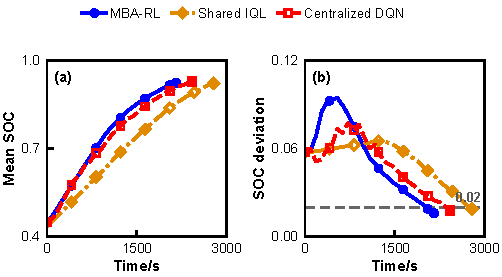
\includegraphics[width=0.95\columnwidth]{comparative_charging_discrete.pdf}
\caption{Representative charging trajectories for the discrete-action methods.}
\label{fig:discrete_trajectories}
\end{figure}

\begin{table}[!t]
\centering
\caption{Learned-method performance over unseen initial-SOC conditions. Values are mean $\pm$ standard deviation across five training runs.}
\label{tab:modern_baselines}
\footnotesize
\setlength{\tabcolsep}{2pt}
\begin{tabular*}{0.98\columnwidth}{@{\extracolsep{\fill}}lcc@{}}
\toprule
Method & Time score (s) & $\int\sigma\,\mathrm{d}t$ \\
 & & (SOC fraction s) \\
\midrule
\multicolumn{3}{@{}l}{\textit{Discrete-action methods}} \\
MBA-RL & $2701.50\pm919.80$ & $205.42\pm57.03$ \\
Shared IQL & $2641.50\pm439.42$ & $235.17\pm69.76$ \\
Centralized DQN & $2673.00\pm73.98$ & $230.35\pm24.20$ \\
Discrete MAPPO & $2340.00\pm347.96$ & $200.83\pm60.75$ \\
\addlinespace[1pt]
\multicolumn{3}{@{}l}{\textit{Continuous-action methods}} \\
Continuous MAPPO & $2698.50\pm154.65$ & $240.36\pm27.58$ \\
SAC & $2173.50\pm157.09$ & $156.04\pm30.74$ \\
\bottomrule
\end{tabular*}
\end{table}

All methods achieve a 100\% task-completion rate except continuous MAPPO, which achieves 98.3\%. Among the value-based methods using the same discrete current set, MBA-RL reduces accumulated SOC imbalance by 12.65\% relative to shared IQL and by 10.82\% relative to centralized DQN, with comparable time scores. Discrete MAPPO and SAC obtain lower numerical scores in Table~\ref{tab:modern_baselines}. The representative trajectories in Fig.~\ref{fig:discrete_trajectories} show the corresponding differences in charging progress and SOC deviation.

\subsubsection{Ablation and Sensitivity Analysis}

The ablation study removes the mixing network, parameter sharing, and balancing reward from MBA-RL, with all variants retrained under the same protocol. Independent IQL, which removes both mixing and parameter sharing, is included as an additional reference. The results are summarized in Fig.~\ref{fig:component_ablation}.

\begin{figure}[!t]
\centering
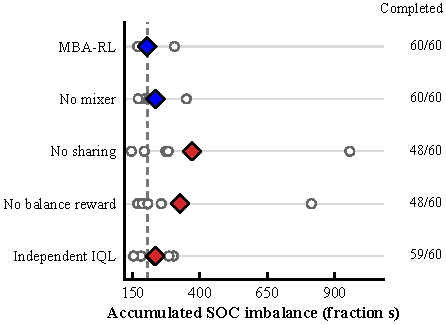
\includegraphics[width=0.95\columnwidth]{component_ablation.pdf}
\caption{Ablation results. Open circles denote training-run means and diamonds overall means; blue diamonds indicate 100\% task completion and red diamonds lower completion rates. The dashed line marks the MBA-RL mean.}
\label{fig:component_ablation}
\end{figure}

Removing parameter sharing or the balancing reward reduces the task-completion rate to 80\% and substantially increases accumulated SOC imbalance. Removing the mixing network retains 100\% completion but increases the accumulated imbalance by about 14\%. Independent IQL also yields a higher accumulated imbalance than MBA-RL. Together, these results show that the observed performance is supported by several components rather than by the mixing network alone.

To examine operating robustness without adaptation, policies trained under nominal conditions are evaluated with fixed weights under parameter, observation, ambient-temperature, and actuation variations. The task-completion rate remains 100\% under the tested $\pm10\%$ parameter variations, fixed sensor bias, a 15~$^\circ$C ambient condition, and a 30\% reduction in available current. Performance decreases under observation noise, a one-decision delay, and ambient temperatures of 34--35~$^\circ$C, indicating greater sensitivity to observation errors, delay, and high-temperature operation than to the tested parameter and actuation variations.

The same MBA-RL architecture was also trained for packs with 3, 6, and 12 independently controlled cells. The task-completion rate decreases from 98.3\% in the three-cell setting to 80.6\% in the 12-cell setting as the pack size increases. Although the computational cost increases with pack size, safety processing remains within the 90 s decision interval at the tested scales. The larger simulated packs are constructed by repeating the three identified cell models and do not include series-circuit, shared-power, or thermal coupling; the scalability results should therefore be interpreted within this simplified setting.
% End merged section: 04_results.tex

% Begin merged section: 05_conclusion.tex
\section{Conclusion}

This paper presented a multi-balancing-agent reinforcement learning (MBA-RL) framework for coordinated lithium-ion battery charging. The charging problem was formulated as a cooperative multi-agent decision process in which each agent regulates the charging current of one cell, while QMIX coordinates the cell-level decisions toward fast charging and pack-level SOC balancing. A model-based safety mechanism was incorporated to screen the requested currents against predicted voltage, temperature, and SOC limits before execution. By coordinating nonnegative cell-level charging currents, the proposed framework performs charging and SOC balancing without relying on a dedicated equalization topology.

The evaluation results demonstrate the effectiveness of the proposed framework under the tested conditions. Compared with shared independent Q-learning and centralized DQN using the same discrete current set, MBA-RL reduces accumulated SOC imbalance by 12.65\% and 10.82\%, respectively. The model-based safety mechanism improves constraint satisfaction to 100\% in the reported safety tests, while incorporating the same mechanism during training further improves task completion. The ablation and sensitivity studies also confirm the importance of parameter sharing and the balancing reward and reveal the sensitivity of the learned policy to observation errors and high ambient temperatures.

Future work will focus on validating the proposed charging controller using independent charging measurements and hardware-in-the-loop experiments. The framework will also be extended to larger battery packs with shared electrical, power, and thermal constraints and to more reliable state estimation and uncertainty-aware control.
% End merged section: 05_conclusion.tex


% References embedded for a complete single-file source.
% Generated by IEEEtran.bst, version: 1.14 (2015/08/26)
\begin{thebibliography}{10}
\providecommand{\url}[1]{#1}
\csname url@samestyle\endcsname
\providecommand{\newblock}{\relax}
\providecommand{\bibinfo}[2]{#2}
\providecommand{\BIBentrySTDinterwordspacing}{\spaceskip=0pt\relax}
\providecommand{\BIBentryALTinterwordstretchfactor}{4}
\providecommand{\BIBentryALTinterwordspacing}{\spaceskip=\fontdimen2\font plus
\BIBentryALTinterwordstretchfactor\fontdimen3\font minus
  \fontdimen4\font\relax}
\providecommand{\BIBforeignlanguage}[2]{{%
\expandafter\ifx\csname l@#1\endcsname\relax
\typeout{** WARNING: IEEEtran.bst: No hyphenation pattern has been}%
\typeout{** loaded for the language `#1'. Using the pattern for}%
\typeout{** the default language instead.}%
\else
\language=\csname l@#1\endcsname
\fi
#2}}
\providecommand{\BIBdecl}{\relax}
\BIBdecl

\bibitem{1}
L.~H. Saw, Y.~Ye, and A.~A. Tay, ``Integration issues of lithium-ion battery
  into electric vehicles battery pack,'' \emph{Journal of Cleaner Production},
  vol. 113, pp. 1032--1045, 2016.

\bibitem{3}
N.~Tashakor, E.~Farjah, and T.~Ghanbari, ``A bidirectional battery charger with
  modular integrated charge equalization circuit,'' \emph{IEEE Transactions on
  Power Electronics}, vol.~32, no.~3, pp. 2133--2145, 2016.

\bibitem{4}
F.~Feng, X.~Hu, J.~Liu, X.~Lin, and B.~Liu, ``A review of equalization
  strategies for series battery packs: variables, objectives, and algorithms,''
  \emph{Renewable and Sustainable Energy Reviews}, vol. 116, p. 109464, 2019.

\bibitem{liu2024degradation}
\BIBentryALTinterwordspacing
X.~Liu, Z.~Hu, X.~Wang, and M.~Xie, ``Capacity degradation assessment of
  lithium-ion battery considering coupling effects of calendar and cycling
  aging,'' \emph{IEEE Transactions on Automation Science and Engineering},
  vol.~21, no.~3, pp. 3052--3064, 2024. [Online]. Available:
  \url{https://ieeexplore.ieee.org/document/10127965/}
\BIBentrySTDinterwordspacing

\bibitem{duan2026coestimation}
\BIBentryALTinterwordspacing
B.~Duan, H.~Sun, X.~Liu, Y.~Li, K.~Liu, C.~Li, and Y.~Kang, ``The accurate
  co-estimation of state of charge and state of energy for lithium-ion battery
  based on model-data fused framework,'' \emph{IEEE Transactions on Automation
  Science and Engineering}, vol.~23, pp. 10\,438--10\,448, 2026. [Online].
  Available: \url{https://ieeexplore.ieee.org/document/11535486/}
\BIBentrySTDinterwordspacing

\bibitem{fricke2026prognosis}
\BIBentryALTinterwordspacing
K.~Fricke, R.~G. Nascimento, M.~Corbetta, C.~S. Kulkarni, and F.~A.~C. Viana,
  ``Hybrid physics-informed neural networks for prognosis and fleet management
  of {Li-Ion} batteries under large load variations,'' \emph{IEEE Transactions
  on Automation Science and Engineering}, vol.~23, pp. 3829--3842, 2026.
  [Online]. Available: \url{https://ieeexplore.ieee.org/document/11223789/}
\BIBentrySTDinterwordspacing

\bibitem{7}
J.~Cao, N.~Schofield, and A.~Emadi, ``Battery balancing methods: A
  comprehensive review,'' in \emph{2008 IEEE Vehicle Power and Propulsion
  Conference}.\hskip 1em plus 0.5em minus 0.4em\relax IEEE, 2008, pp. 1--6.

\bibitem{8}
M.~Daowd, N.~Omar, P.~Van Den~Bossche, and J.~Van~Mierlo, ``Passive and active
  battery balancing comparison based on matlab simulation,'' in \emph{2011 IEEE
  Vehicle Power and Propulsion Conference}.\hskip 1em plus 0.5em minus
  0.4em\relax IEEE, 2011, pp. 1--7.

\bibitem{9}
F.~Baronti, R.~Roncella, and R.~Saletti, ``Performance comparison of active
  balancing techniques for lithium-ion batteries,'' \emph{Journal of Power
  Sources}, vol. 267, pp. 603--609, 2014.

\bibitem{10}
N.~Ghaeminezhad, Q.~Ouyang, X.~Hu, G.~Xu, and Z.~Wang, ``Active cell
  equalization topologies analysis for battery packs: A systematic review,''
  \emph{IEEE Transactions on Power Electronics}, vol.~36, no.~8, pp.
  9119--9135, 2021.

\bibitem{11}
S.~Yarlagadda, T.~T. Hartley, and I.~Husain, ``A battery management system
  using an active charge equalization technique based on a dc/dc converter
  topology,'' \emph{IEEE Transactions on Industry Applications}, vol.~49,
  no.~6, pp. 2720--2729, 2013.

\bibitem{12}
T.~Duraisamy and D.~Kaliyaperumal, ``Adaptive passive balancing in battery
  management system for e-mobility,'' \emph{International Journal of Energy
  Research}, vol.~45, no.~7, pp. 10\,752--10\,764, 2021.

\bibitem{13}
I.~Aizpuru, U.~Iraola, J.~Canales, M.~Echeverria, and I.~Gil, ``Passive
  balancing design for li-ion battery packs based on single cell experimental
  tests for a cccv charging mode,'' in \emph{2013 International Conference on
  Clean Electrical Power (ICCEP)}.\hskip 1em plus 0.5em minus 0.4em\relax IEEE,
  2013, pp. 93--98.

\bibitem{14}
M.~Hoque, M.~Hannan, and A.~Mohamed, ``Optimal cc-cv charging of lithium-ion
  battery for charge equalization controller,'' in \emph{2016 International
  Conference on Advances in Electrical, Electronic and Systems Engineering
  (ICAEES)}.\hskip 1em plus 0.5em minus 0.4em\relax IEEE, 2016, pp. 610--615.

\bibitem{15}
Y.-S. Lee and M.-W. Cheng, ``Intelligent control battery equalization for
  series connected lithium-ion battery strings,'' \emph{IEEE Transactions on
  Industrial Electronics}, vol.~52, no.~5, pp. 1297--1307, 2005.

\bibitem{16}
T.-E. Fan, S.-M. Liu, H.~Yang, P.-H. Li, and B.~Qu, ``A fast active balancing
  strategy based on model predictive control for lithium-ion battery packs,''
  \emph{Energy}, vol. 279, p. 128028, 2023.

\bibitem{chen2024balancing}
\BIBentryALTinterwordspacing
J.~Chen, A.~Behal, Z.~Li, and C.~Li, ``Active battery cell balancing by
  real-time model predictive control for extending electric vehicle driving
  range,'' \emph{IEEE Transactions on Automation Science and Engineering},
  vol.~21, no.~3, pp. 4003--4015, 2024. [Online]. Available:
  \url{https://ieeexplore.ieee.org/document/10176298/}
\BIBentrySTDinterwordspacing

\bibitem{yan2026bess}
\BIBentryALTinterwordspacing
C.~Yan, X.~Sun, X.~Zhang, T.~Cheng, and J.~Gu, ``Prescribed performance-based
  distributed adaptive predefined-time consensus control for {BESSs},''
  \emph{IEEE Transactions on Automation Science and Engineering}, vol.~23, pp.
  10\,640--10\,655, 2026. [Online]. Available:
  \url{https://ieeexplore.ieee.org/document/11516203/}
\BIBentrySTDinterwordspacing

\bibitem{pozzi2023dagger}
A.~Pozzi and D.~Toti, ``Imitation learning for agnostic battery charging: A
  dagger-based approach,'' \emph{IEEE Access}, vol.~11, pp. 115\,190--115\,203,
  2023.

\bibitem{pozzi2025stochastic}
A.~Pozzi, A.~Incremona, and D.~Toti, ``Neural network-based imitation learning
  for approximating stochastic battery management systems,'' \emph{IEEE
  Access}, vol.~13, pp. 71\,041--71\,052, 2025.

\bibitem{dong2025charging}
\BIBentryALTinterwordspacing
X.~Dong, H.~Xv, T.~Pan, X.~Liu, J.~Tian, and P.~Wang, ``Multi-objective
  charging optimization of lithium-ion batteries considering electrical,
  thermal, and aging behaviors using deep reinforcement learning,'' \emph{IEEE
  Transactions on Automation Science and Engineering}, vol.~22, pp.
  18\,493--18\,508, 2025. [Online]. Available:
  \url{https://ieeexplore.ieee.org/document/11079681/}
\BIBentrySTDinterwordspacing

\bibitem{17}
Y.~Yang, J.~He, C.~Chen, and J.~Wei, ``Balancing awareness fast charging
  control for lithium-ion battery pack using deep reinforcement learning,''
  \emph{IEEE Transactions on Industrial Electronics}, vol.~71, no.~4, pp.
  3718--3727, 2023.

\bibitem{18}
C.~Lu, J.~Chen, C.~Chen, Y.~Huang, and D.~Xuan, ``An active equalization method
  for redundant battery based on deep reinforcement learning,''
  \emph{Measurement}, vol. 210, p. 112507, 2023.

\bibitem{19}
L.~Busoniu, R.~Babuska, and B.~De~Schutter, ``A comprehensive survey of
  multiagent reinforcement learning,'' \emph{IEEE Transactions on Systems, Man,
  and Cybernetics, Part C (Applications and Reviews)}, vol.~38, no.~2, pp.
  156--172, 2008.

\bibitem{20}
K.~Zhang, Z.~Yang, and T.~Ba{\c{s}}ar, ``Multi-agent reinforcement learning: A
  selective overview of theories and algorithms,'' \emph{Handbook of
  reinforcement learning and control}, pp. 321--384, 2021.

\bibitem{21}
Y.~Liang, Z.~Ding, T.~Zhao, and W.-J. Lee, ``Real-time operation management for
  battery swapping-charging system via multi-agent deep reinforcement
  learning,'' \emph{IEEE Transactions on Smart Grid}, vol.~14, no.~1, pp.
  559--571, 2022.

\bibitem{22}
J.~Dong, A.~Yassine, A.~Armitage, and M.~S. Hossain, ``Multi-agent
  reinforcement learning for intelligent v2g integration in future
  transportation systems,'' \emph{IEEE Transactions on Intelligent
  Transportation Systems}, 2023.

\bibitem{tavakol2025marl}
Y.~Tavakol-Moghaddam and M.~Boroushaki, ``A multi-agent reinforcement learning
  approach for continuous battery cell-level balancing,'' \emph{Results in
  Engineering}, vol.~26, p. 104898, 2025.

\bibitem{23}
H.~Perez, S.~Dey, X.~Hu, and S.~Moura, ``Optimal charging of li-ion batteries
  via a single particle model with electrolyte and thermal dynamics,''
  \emph{Journal of The Electrochemical Society}, vol. 164, no.~7, p. A1679,
  2017.

\bibitem{25}
S.~G. Marquis, V.~Sulzer, R.~Timms, C.~P. Please, and S.~J. Chapman, ``An
  asymptotic derivation of a single particle model with electrolyte,''
  \emph{Journal of The Electrochemical Society}, vol. 166, no.~15, p. A3693,
  2019.

\bibitem{26}
T.~Rashid, M.~Samvelyan, C.~S. De~Witt, G.~Farquhar, J.~Foerster, and
  S.~Whiteson, ``Monotonic value function factorisation for deep multi-agent
  reinforcement learning,'' \emph{Journal of Machine Learning Research},
  vol.~21, no. 178, pp. 1--51, 2020.

\bibitem{27}
F.~A. Oliehoek, C.~Amato \emph{et~al.}, \emph{A concise introduction to
  decentralized POMDPs}.\hskip 1em plus 0.5em minus 0.4em\relax Springer, 2016,
  vol.~1.

\bibitem{zou2019sufficient}
F.~Zou, L.~Shen, Z.~Jie, W.~Zhang, and W.~Liu, ``A sufficient condition for
  convergences of adam and rmsprop,'' in \emph{Proceedings of the IEEE/CVF
  Conference on Computer Vision and Pattern Recognition}, 2019, pp.
  11\,127--11\,135.

\bibitem{28}
M.~A. Rahman, S.~Anwar, and A.~Izadian, ``Electrochemical model parameter
  identification of a lithium-ion battery using particle swarm optimization
  method,'' \emph{Journal of Power Sources}, vol. 307, pp. 86--97, 2016.

\bibitem{29}
V.~Sulzer, S.~G. Marquis, R.~Timms, M.~Robinson, and S.~J. Chapman, ``Python
  battery mathematical modelling (pybamm),'' \emph{Journal of Open Research
  Software}, vol.~9, no. 1, Article 14, 2021.

\bibitem{mnih2015dqn}
V.~Mnih, K.~Kavukcuoglu, D.~Silver, A.~A. Rusu, J.~Veness, M.~G. Bellemare,
  A.~Graves, M.~Riedmiller, A.~K. Fidjeland, G.~Ostrovski, S.~Petersen,
  C.~Beattie, A.~Sadik, I.~Antonoglou, H.~King, D.~Kumaran, D.~Wierstra,
  S.~Legg, and D.~Hassabis, ``Human-level control through deep reinforcement
  learning,'' \emph{Nature}, vol. 518, no. 7540, pp. 529--533, 2015.

\bibitem{yu2022mappo}
C.~Yu, A.~Velu, E.~Vinitsky, J.~Gao, Y.~Wang, A.~Bayen, and Y.~Wu, ``The
  surprising effectiveness of ppo in cooperative multi-agent games,'' in
  \emph{Advances in Neural Information Processing Systems}, vol.~35, 2022, pp.
  24\,611--24\,624.

\bibitem{haarnoja2018sac}
T.~Haarnoja, A.~Zhou, P.~Abbeel, and S.~Levine, ``Soft actor-critic: Off-policy
  maximum entropy deep reinforcement learning with a stochastic actor,'' in
  \emph{Proceedings of the 35th International Conference on Machine Learning},
  ser. Proceedings of Machine Learning Research, vol.~80, 2018, pp. 1861--1870.

\end{thebibliography}

\end{document}
